\documentclass[12pt]{report}
\usepackage[utf8]{inputenc}
\usepackage[T1]{fontenc}  % Added for better font encoding
\usepackage{graphicx}
\usepackage[hidelinks]{hyperref}
\usepackage{longtable}
\usepackage{listings}
\usepackage{amsmath}
\usepackage{geometry}
\usepackage{algorithm}       
\usepackage{algpseudocode}
\usepackage{float}
\usepackage{adjustbox}
\usepackage{caption}
\usepackage{array}
\usepackage{ragged2e}
\usepackage{subcaption}
\usepackage{placeins}
\usepackage{xcolor}  % Added for code coloring
\usepackage{tcolorbox}  % Added for colored boxes
\tcbuselibrary{skins}  % Added for additional box styles

% NEW PACKAGES FOR TREE STRUCTURES
\usepackage{forest}  % For professional tree structures
\usepackage{tikz}    % For custom tree drawings
\usetikzlibrary{trees}

% Configure tcolorbox style
\tcbset{
    enhanced,
    colback=blue!5!white,        % Light blue background instead of white
    colframe=blue!70!black,      % Darker frame for better visibility
    coltitle=black,              % BLACK TITLE TEXT
    fonttitle=\bfseries,
    boxrule=1pt,                 % Thicker border
    arc=3mm,                     % Slightly more rounded corners
    title style={fill=white},    % WHITE TITLE BACKGROUND
    attach title to upper,
    drop shadow,                 % Add shadow for better visibility
    before skip=10pt,            % Space before box
    after skip=10pt              % Space after box
}

% Additional tcolorbox styles for different purposes
\newtcolorbox{architecturebox}[1][]{
    enhanced,
    colback=blue!8!white,
    colframe=blue!75!black,
    coltitle=black,              % BLACK TITLE TEXT
    fonttitle=\bfseries\large,
    boxrule=1.5pt,
    arc=3mm,
    title style={fill=white},    % WHITE TITLE BACKGROUND
    drop shadow={opacity=0.3},
    before skip=15pt,
    after skip=15pt,
    #1
}

\newtcolorbox{highlightbox}[1][]{
    enhanced,
    colback=gray!10!white,
    colframe=gray!60!black,
    coltitle=black,              % BLACK TITLE TEXT
    fonttitle=\bfseries,
    boxrule=1pt,
    arc=2mm,
    title style={fill=white},    % WHITE TITLE BACKGROUND
    drop shadow={opacity=0.2},
    before skip=10pt,
    after skip=10pt,
    #1
}

% Fix for UTF-8 encoding in listings
\lstset{
    extendedchars=true,
    inputencoding=utf8,
    literate={é}{{\'e}}1 {è}{{\`e}}1 {ê}{{\^e}}1 {ë}{{\"e}}1
             {É}{{\'E}}1 {È}{{\`E}}1 {Ê}{{\^E}}1 {Ë}{{\"E}}1
             {à}{{\`a}}1 {â}{{\^a}}1 {ä}{{\"a}}1
             {À}{{\`A}}1 {Â}{{\^A}}1 {Ä}{{\"A}}1
             {ç}{{\c{c}}}1 {Ç}{{\c{C}}}1
             {œ}{{\oe}}1 {Œ}{{\OE}}1
             {ù}{{\`u}}1 {û}{{\^u}}1 {ü}{{\"u}}1
             {Ù}{{\`U}}1 {Û}{{\^U}}1 {Ü}{{\"U}}1
             {î}{{\^i}}1 {ï}{{\"i}}1
             {Î}{{\^I}}1 {Ï}{{\"I}}1
             {ô}{{\^o}}1 {ö}{{\"o}}1
             {Ô}{{\^O}}1 {Ö}{{\"O}}1
}

% Code styling configuration
\definecolor{codegreen}{rgb}{0,0.6,0}
\definecolor{codegray}{rgb}{0.5,0.5,0.5}
\definecolor{codepurple}{rgb}{0.58,0,0.82}
\definecolor{backcolour}{rgb}{0.95,0.95,0.92}

% Define code style
\lstdefinestyle{mystyle}{
    backgroundcolor=\color{backcolour},   
    commentstyle=\color{codegreen},
    keywordstyle=\color{magenta},
    numberstyle=\tiny\color{codegray},
    stringstyle=\color{codepurple},
    basicstyle=\ttfamily\footnotesize,
    breakatwhitespace=false,         
    breaklines=true,                 
    captionpos=b,                    
    keepspaces=true,                 
    numbers=left,                    
    numbersep=5pt,                  
    showspaces=false,                
    showstringspaces=false,
    showtabs=false,                  
    tabsize=2,
    frame=single,
    xleftmargin=2em,
    xrightmargin=2em
}

% ENHANCED DIRECTORY TREE STYLE FOR LISTINGS
\lstdefinestyle{treestyle}{
    backgroundcolor=\color{backcolour},   
    commentstyle=\color{codegreen},
    basicstyle=\ttfamily\small,
    breakatwhitespace=false,         
    breaklines=true,                 
    captionpos=b,                    
    keepspaces=true,                 
    numbers=left,                    
    numbersep=5pt,                  
    showspaces=false,                
    showstringspaces=false,
    showtabs=false,                  
    tabsize=2,
    frame=single,
    xleftmargin=1em,
    xrightmargin=1em,
    aboveskip=10pt,
    belowskip=10pt
}

\lstset{style=mystyle}

% CUSTOM FOREST STYLE FOR DIRECTORY TREES
\forestset{
    directory tree/.style={
        for tree={
            font=\ttfamily,
            grow'=0,
            child anchor=west,
            parent anchor=south,
            anchor=west,
            calign=first,
            edge path={
                \noexpand\path [draw, \forestoption{edge}]
                (!u.south west) +(7.5pt,0) |- node[fill,inner sep=1.25pt] {} (.child anchor)\forestoption{edge label};
            },
            before typesetting nodes={
                if n=1
                    {insert before={[,phantom]}}
                    {}
            },
            fit=band,
            before computing xy={l=15pt},
        }
    }
}

% CUSTOM COMMAND FOR SIMPLE DIRECTORY LISTINGS
\newcommand{\dirtree}[1]{%
    \begin{lstlisting}[style=treestyle, mathescape=false]
#1
    \end{lstlisting}
}

% Improved image placement settings
\setcounter{topnumber}{2}
\setcounter{bottomnumber}{2}
\setcounter{totalnumber}{4}
\renewcommand{\topfraction}{0.85}
\renewcommand{\bottomfraction}{0.85}
\renewcommand{\textfraction}{0.15}
\renewcommand{\floatpagefraction}{0.85}
\setlength{\floatsep}{3pt plus 1pt minus 1pt}        % Reduced spacing between floats
\setlength{\textfloatsep}{3pt plus 1pt minus 1pt}    % Reduced spacing between text and floats
\setlength{\intextsep}{3pt plus 1pt minus 1pt}       % Reduced spacing for in-text floats


% Force figures to stay in their sections
\let\origfigure\figure
\let\endorigfigure\endfigure
\renewenvironment{figure}[1][]{%
    \origfigure[#1]%
    \setlength{\abovecaptionskip}{10pt}%
    \setlength{\belowcaptionskip}{10pt}%
}{%
    \endorigfigure%
}

\captionsetup[table]{skip=10pt, labelfont=bf, labelsep=colon}
\geometry{a4paper, margin=1in}
\renewcommand{\bibname}{References}
\renewcommand{\algorithmicrequire}{\textbf{Input:}}
\renewcommand{\algorithmicensure}{\textbf{Output:}}
\newcolumntype{C}[1]{>{\centering\arraybackslash}p{#1}} 
\newcolumntype{L}[1]{>{\raggedright\arraybackslash}p{#1}} 
\newcolumntype{P}[1]{>{\RaggedRight\arraybackslash}p{#1}} 

% Dart language definition
\lstdefinelanguage{Dart}{
  morekeywords={
    abstract, as, assert, async, await, break, case, catch, class, const,
    continue, covariant, default, deferred, do, else, enum, export, extends,
    extension, external, factory, false, final, finally, for, Function, get,
    hide, if, implements, import, in, interface, is, late, library, mixin, new,
    null, on, operator, part, required, rethrow, return, set, show, static,
    super, switch, sync, this, throw, true, try, typedef, var, void, while,
    with, yield
  },
  sensitive=true,
  morecomment=[l]{//},
  morecomment=[s]{/*}{*/},
  morestring=[b]",
  morestring=[b]',
}

% TypeScript language definition
\lstdefinelanguage{TypeScript}{
  morekeywords={
    abstract, any, as, asserts, bigint, boolean, break, case, catch, class,
    const, constructor, continue, debugger, declare, default, delete, do,
    else, enum, export, extends, false, finally, for, from, function, get,
    if, implements, import, in, infer, instanceof, interface, is, keyof,
    let, module, namespace, never, new, null, number, object, of, package,
    private, protected, public, readonly, require, return, set, static,
    string, super, switch, symbol, this, throw, true, try, type, typeof,
    undefined, unique, unknown, var, void, while, with, yield
  },
  sensitive=true,
  morecomment=[l]{//},
  morecomment=[s]{/*}{*/},
  morestring=[b]",
  morestring=[b]',
}



\begin{document}  % <-- This must come before content 

\begin{titlepage}
    \thispagestyle{empty}

    % Logos
    \begin{minipage}{0.49\textwidth}
        \raggedright
        
\includegraphics[width=2.5cm]{images/university_logo.png}
    \end{minipage}
    \begin{minipage}{0.49\textwidth}
        \raggedleft
        
\includegraphics[width=2.5cm]{images/faculty_logo.png}
    \end{minipage}

    \vspace{2cm}

    \begin{center}
        {\LARGE \textbf{Damanhour University}}\\[0.5em]
        {\Large \textbf{Faculty of Computers and Information}}\\[1.5cm]

        {\Larg{Project II}}\\e \textbf[0.5em]
        {\Huge \textbf{Student Portal}}\\[1.5cm]

        {\Large \textbf{Team Members}}\\[1em]
        \begin{center}
        \makebox[0.9\textwidth]{% reduce width to tighten layout
            \begin{minipage}{0.48\textwidth}
                \centering
                Tasbeeh Ismail \\
                Nour Allam \\
                Abdul Rahman Abu Zied \\
                Abdul Rahman Ahmed Saad \\
                Mo'men Ayman \\
            \end{minipage}
            \begin{minipage}{0.48\textwidth}
                \centering
                Omnia Gamal \\
                Mina Zarif \\
                Youssef Abdelmaksod \\
                Mona Alhusseiny \\
                Abdullah Mohammed \\
                Ziad Ahmed \\
            \end{minipage}
        }
        \end{center}
        

        \vspace{2cm}
        {\Large \textbf{Supervisors}}\\[1em]
        Dr. Nora Shoaip\\
        Dr. Ebtsam Adel\\
        Eng. Abdelrahman Khaled

        \vfill
        {\large \textbf{Jun. 2025}}
    \end{center}
\end{titlepage}

\tableofcontents
\listoffigures
\listoftables

% Include content chapters
\chapter{Introduction}

\section{Motivation}

Students often struggle with fragmented educational platforms, making it difficult to access resources, find mentorship, plan events, and build a collaborative academic community. A unified system that integrates all these functionalities can significantly enhance the student experience by streamlining academic collaboration, improving communication, and fostering knowledge sharing.

\section{Problem Statement}

Despite the growing integration of technology in education, existing platforms lack efficiency in academic collaboration, resource sharing, and mentorship opportunities.

Key challenges include:
\begin{itemize}
    \item Inefficient event organization and communication.
    \item Lack of tools for student collaboration.
    \item Slow access to college and student affairs announcements.
    \item No personalized learning experiences.
\end{itemize}

\section{Goals of the Project}

\begin{itemize}
    \item \textbf{AI-Powered Chatbot:} Provide instant responses to student queries.
    \item \textbf{Event Planner:} Track and recommend academic events.
    \item \textbf{Knowledge-Sharing Ecosystem:} Upload, discover, and share study materials.
    \item \textbf{Mentorship \& Collaboration:} Facilitate student-peer, faculty, and alumni interactions.
    \item \textbf{Personalized Learning Recommendations:} Enhance guidance and support.
    \item \textbf{Real-Time Notifications:} Ensure faster and easier access to announcements.
\end{itemize}

\section{Software Development Methodology}

\textbf{Agile Software Development} was chosen due to its flexibility, iterative approach, and ability to adapt to changing requirements.

Advantages of Agile:
\begin{itemize}
    \item Continuous feedback loops for better user experience.
    \item Frequent testing and debugging to ensure system reliability.
    \item Seamless collaboration between developers, designers, and stakeholders.
    \item Risk management by identifying technical and performance bottlenecks early.
\end{itemize}

\chapter{Literature Review}

\section{Feature Matrix}

\begin{longtable}{|L{2cm}|C{2.2cm}|C{2cm}|L{4cm}|L{2.5cm}|}
\hline
\textbf{Feature Module} & \textbf{Importance} & \textbf{Effort} & \textbf{Impact} & \textbf{Stakeholders} \\
\hline
User Authentication & High & Medium & Enables secure access and personalized usage & Students, Faculty, Admins \\
\hline
Profile Management & High & Medium & Personalizes user experience and information & Students, Faculty \\
\hline
View Events & High & Low & Helps students stay updated on academic events & Students \\
\hline
RSVP for Events & Medium & Low & Encourages participation in academic activities & Students, Admins \\
\hline
Sync with Personal Calendars & Medium & Medium & Enhances user experience through integration & Students, Faculty \\
\hline
AI-Suggested Events & Medium (Future Plan) & High & Personalizes event recommendations & Students \\
\hline
Resource Sharing & High & Medium & Facilitates collaboration and knowledge sharing & Students, Faculty \\
\hline
Categorized Content Upload & Medium & Medium & Streamlines content organization and discovery & Students \\
\hline
Participate in Discussions & High & High & Encourages collaboration and community building & Students \\
\hline
AI-Powered Chatbot (FAQ) & High & Medium & Responds to common institutional queries & Students, Admins \\
\hline
NLP-Based Suggestions & Medium & High & Personalizes responses to complex queries & Students, Admins \\
\hline
Recommendation Engine & Medium (Future Plan) & High & Provides personalized content recommendations & Students \\
\hline
Post Suggestions & Medium (Future Plan) & High & Improves engagement with academic content & Students \\
\hline
Mentorship Matching & High & Medium & Connects students with mentors for guidance & Students, Faculty \\
\hline
Direct Messaging & Medium & Medium & Enables communication between mentors/mentees & Students, Faculty \\
\hline
Announcements Dashboard & High & Medium & Centralizes important updates and notifications & Students, Faculty \\
\hline
Real-Time Notifications & High & Medium & Keeps users informed about updates/events & Students \\
\hline
\end{longtable}

\section{Comparison of Existing Solutions with the Proposed Solution}

Most existing platforms like Microsoft Teams, Moodle, and Blackboard Learn offer basic collaboration tools, but they lack personalized AI recommendations, effective mentorship systems, and a centralized student affairs integration.

\subsection*{Key Advantages of the Proposed Student Portal}

\begin{enumerate}
    \item \textbf{AI-Powered Chatbot:} Unlike existing solutions, our system provides real-time responses to student queries.
    \item \textbf{Comprehensive Event Management:} Full-featured event planner with RSVP tracking and AI-powered recommendations.
    \item \textbf{Personalized Learning Experience:} AI-driven content recommendations tailored to student needs.
    \item \textbf{Enhanced Mentorship System:} Built-in mentorship matching and direct communication tools.
    \item \textbf{Centralized Notifications \& Dashboard:} A single hub for announcements, reducing communication delays.
    \item \textbf{Seamless Community Collaboration:} Interactive discussion forums and categorized knowledge-sharing spaces.
    \item \textbf{Student Affairs Integration:} Direct integration with academic administration for instant updates.
\end{enumerate}


\chapter{Requirement Engineering}

\section{Surveys, Questionnaires, and Interviews}

To ensure that the Student Portal design aligns with students' actual needs and expectations, a mixed-method approach involving surveys and interviews was adopted. The goal was to explore students' current challenges with academic platforms and gather actionable insights for feature development.

\subsection*{Survey Findings}

The survey reached a diverse sample of students, yielding the following key insights:

\begin{itemize}
\item \textbf{44.8\%} of students reported a lack of personalized learning recommendations, making it harder to access relevant academic content efficiently.
\item \textbf{48.0\%} identified limitations in collaboration tools, indicating a need for better features to support group projects and discussion-based learning.
\item \textbf{36.0\%} stated they struggle to access mentorship opportunities, suggesting the portal should integrate features to connect students with mentors more easily.
\item \textbf{31.2\%} expressed frustration over delayed announcements and event updates, showing the importance of real-time notifications and streamlined communication.
\item Additional responses highlighted issues such as poor platform design, difficulty in purchasing educational resources, and general dissatisfaction with usability.
\end{itemize}

\begin{figure}[h]
    \centering
    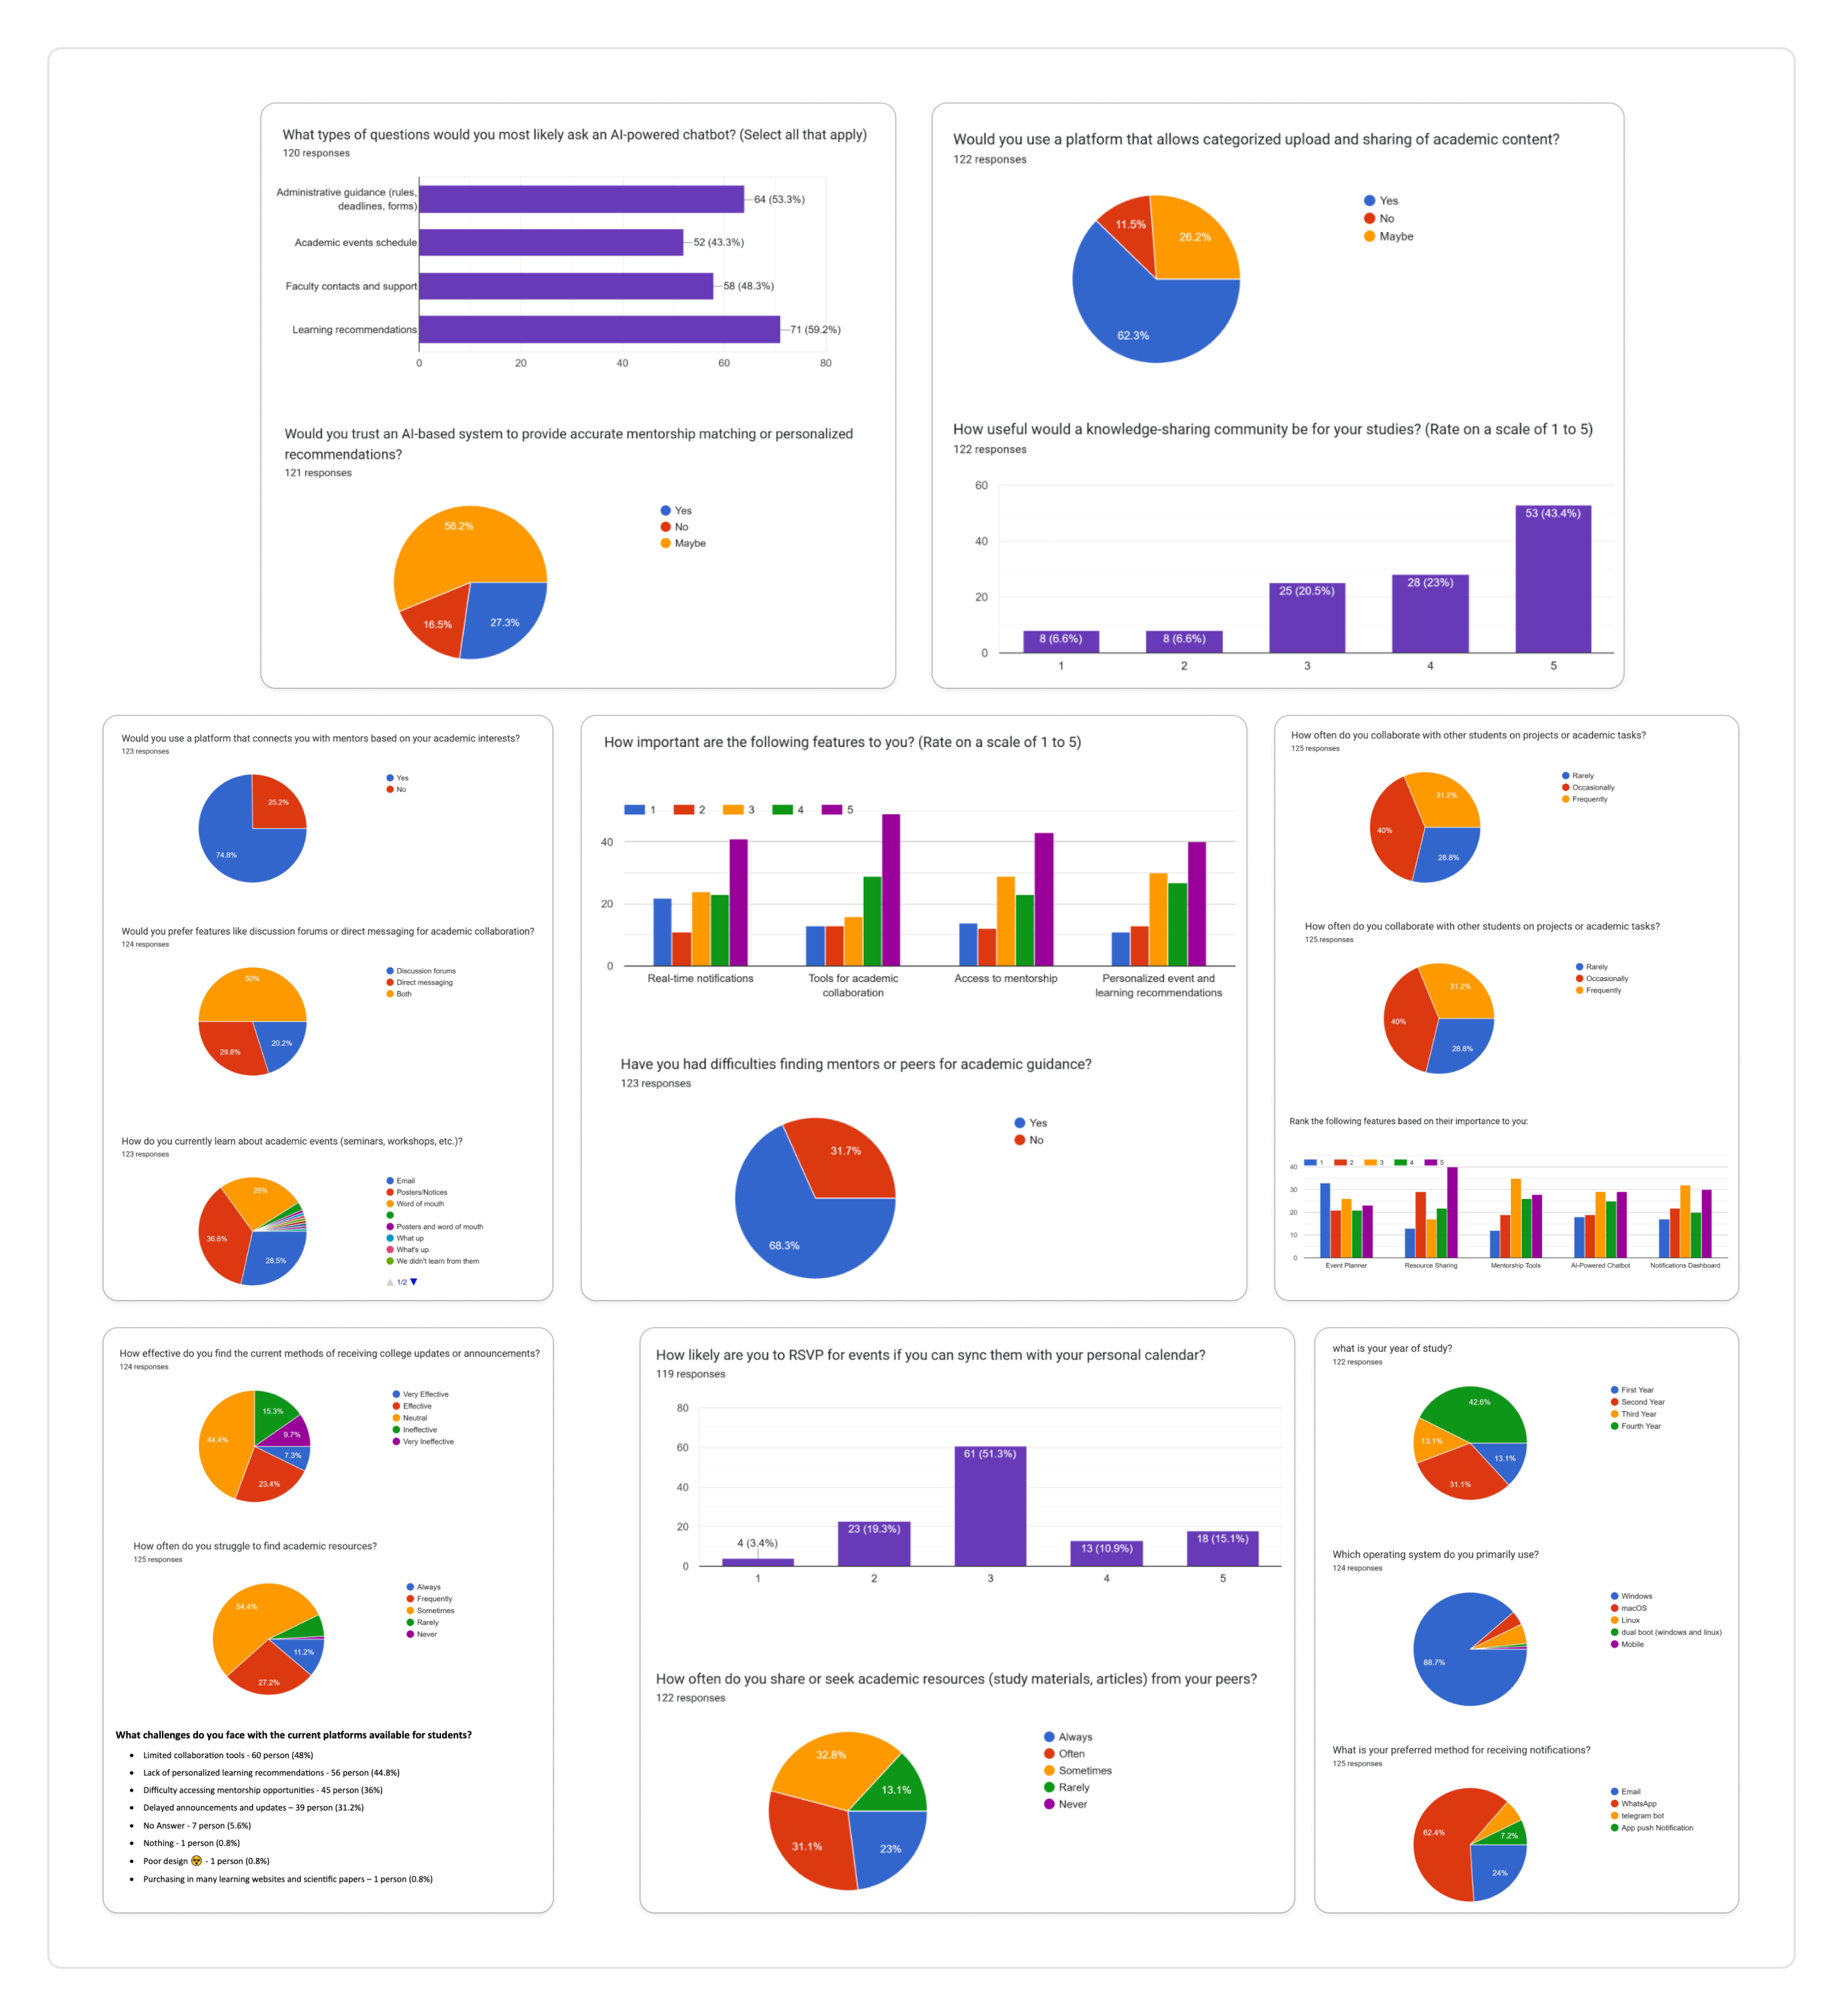
\includegraphics[width=0.8\textwidth]{images/survey_chart.png}
    \caption{Survey Results: Student Challenges with Current Academic Platforms}
    \label{fig:survey_chart}
\end{figure}

\subsection*{Key Questions in Surveys and Interviews}

The data was collected through thoughtfully structured open and closed-ended questions. Some of the most impactful questions included:

\begin{enumerate}
\item What are the biggest challenges in using current academic platforms?
\item Would you benefit from an AI chatbot for quick university-related queries?
\item How do you currently find and attend academic events?
\item Do you feel mentorship opportunities are easily accessible?
\item What additional features would improve your academic experience?
\end{enumerate}

\subsection*{User-Suggested Features and Insights}

Open-ended responses offered rich feedback and creative suggestions. A recurring theme was the demand for an intelligent, supportive, and user-friendly digital environment. Commonly suggested features included:

\begin{itemize}
\item \textbf{AI Chatbot}: To answer questions, recommend resources, send notifications, help with academic system navigation, and track learning progress weekly.
\item \textbf{Improved UX and Responsiveness}: Ease of use and accessibility were considered essential by multiple respondents.
\item \textbf{Media Player Integration}: To simplify access to video lectures and multimedia resources.
\item \textbf{OCR and PDF Analysis Tools}: For better interaction with academic documents.
\item \textbf{Study Planning and Time Management}: Tools to help students manage their workload and plan effectively.
\item \textbf{Mentorship and Peer Support}: Features to connect students with seniors, mentors, and professionals in their field.
\item \textbf{Centralized Academic Resources}: Including Google Drive-like repositories and previous-year materials.
\item \textbf{Event and Quiz Alerts}: Automated email or message notifications to keep students informed in real time.
\end{itemize}

These findings directly informed the functional and non-functional requirements of the portal, ensuring student feedback played a central role in system design.

\subsection*{Emotional Tone and Trust}

Lastly, many students expressed enthusiasm and hope that this platform would surpass current tools like Thinki, noting a desire for a ``platform that can be fully relied upon with artificial intelligence'' and praising the initiative. One respondent wrote:

\begin{quote}
``I trust you and I am looking forward to completing the rest of my university years on your wonderful platform.'' --- \textit{Moamen Sakr, Preparatory Class, Damanhour Engineering}
\end{quote}

Such testimonials underscore the responsibility and potential impact of delivering a well-engineered, student-centric platform.


\section{Functional Requirements}

These are the core features the Student Portal must support:

\begin{enumerate}
    \item \textbf{User Authentication \& Profile Management}
    \begin{itemize}
        \item Secure login with JWT authentication.
        \item Role-based access (Students, Faculty, Admins).
    \end{itemize}

    \item \textbf{AI-Powered Chatbot}
    \begin{itemize}
        \item Answer FAQs related to courses, deadlines, and campus facilities.
        \item Provide academic and administrative guidance.
    \end{itemize}

    \item \textbf{Event Management System}
    \begin{itemize}
        \item Event creation, RSVPs, and calendar synchronization.
        \item AI recommendations for relevant academic events.
    \end{itemize}

    \item \textbf{Resource Sharing \& Knowledge Base}
    \begin{itemize}
        \item Upload/download study materials and academic articles.
        \item AI-driven recommendations based on user activity.
    \end{itemize}

    \item \textbf{Mentorship Matching \& Direct Messaging}
    \begin{itemize}
        \item Match students with faculty or peer mentors.
        \item Real-time messaging and discussion groups.
    \end{itemize}

    \item \textbf{Real-Time Notifications \& Dashboard}
    \begin{itemize}
        \item Instant alerts for announcements, deadlines, and events.
        \item Customizable notifications based on user preferences.
    \end{itemize}

    \item \textbf{Collaboration Tools \& Community Forum}
    \begin{itemize}
        \item Discussion boards for academic topics and group projects.
        \item Categorized Q\&A forums for better engagement.
    \end{itemize}
\end{enumerate}

\section{Non-Functional Requirements}

These define the quality attributes of the system:

\begin{enumerate}
    \item \textbf{Performance}
    \begin{itemize}
        \item The system should handle 1,000+ concurrent users without lag.
        \item AI chatbot responses must be under 2 seconds.
    \end{itemize}

    \item \textbf{Scalability}
    \begin{itemize}
        \item Cloud-based infrastructure to support increasing student enrollment.
        \item Modular architecture for adding future features.
    \end{itemize}

    \item \textbf{Security}
    \begin{itemize}
        \item Data encryption using AES-256 and TLS 1.3.
        \item Secure API gateway with rate limiting and JWT validation.
    \end{itemize}

    \item \textbf{Usability}
    \begin{itemize}
        \item Intuitive UI/UX design for seamless experience on web and mobile.
        \item Minimal onboarding time with self-explanatory navigation.
    \end{itemize}

    \item \textbf{Reliability \& Availability}
    \begin{itemize}
        \item 99.9\% uptime with automatic failover mechanisms.
        \item Regular backups to prevent data loss.
    \end{itemize}

    \item \textbf{Maintainability}
    \begin{itemize}
        \item Codebase follows modular and well-documented practices.
        \item Version control with GitHub for continuous integration \& deployment.
    \end{itemize}
\end{enumerate}

\section{Use Case Diagram}
\begin{figure}[H]
    \centering
    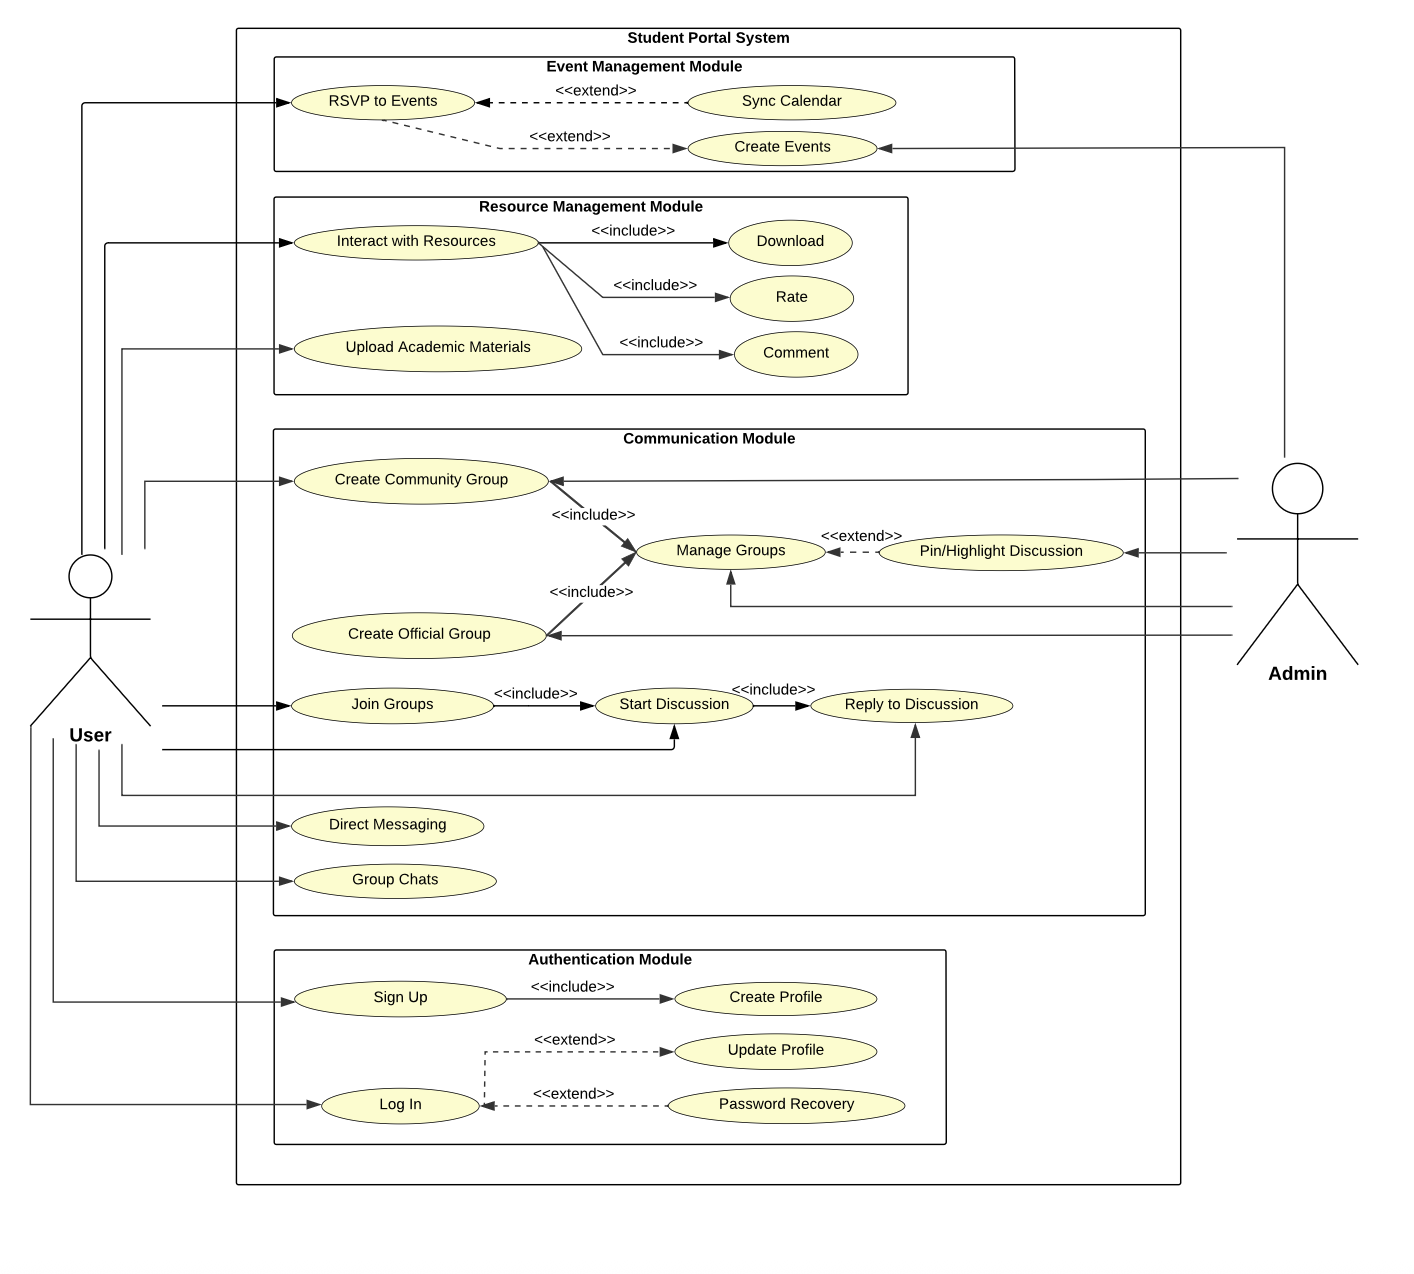
\includegraphics[width=0.8\textwidth]{images/use_case_diagram.png}
    \caption{Student Portal Use Case Diagram}
    \label{fig:use_case}
\end{figure}



\section{Use Case Tables}
\subsubsection{User Management}
\begin{table}[H]
\centering
\caption{UC-101: Sign Up}
\begin{tabular}{|l|p{10cm}|}
\hline
\textbf{Field} & \textbf{Details} \\ \hline
Actor & New User \\ \hline
Trigger & User clicks on the "Sign Up" button \\ \hline
Input & Institutional email, password, optional profile details \\ \hline
Validation Steps & 1. Verify email domain matches institutional pattern \\ 
                 & 2. Ensure password meets security criteria \\ \hline
Error Handling & 1. Display error if email is invalid \\ 
               & 2. Show password validation errors \\ 
               & 3. Alert if email is already registered \\ \hline
Output & User receives a confirmation email \\ \hline
Post-condition & Account is created and active \\ \hline
Priority & High \\ \hline
\end{tabular}
\end{table}

\begin{table}[H]
\centering
\caption{UC-102: Log In}
\begin{tabular}{|l|p{10cm}|}
\hline
\textbf{Field} & \textbf{Details} \\ \hline
Actor & Registered User \\ \hline
Trigger & User clicks "Log In" and enters credentials \\ \hline
Input & Email, password \\ \hline
Validation Steps & Match email and password to stored credentials \\ \hline
Error Handling & 1. Show "Invalid credentials" \\ 
               & 2. Account lock after multiple failed attempts \\ \hline
Output & User gains access to the dashboard \\ \hline
Post-condition & User is logged into their profile \\ \hline
Priority & High \\ \hline
\end{tabular}
\end{table}

% UC-103: Password Recovery
\begin{table}[H]
\centering
\caption{UC-103: Password Recovery}
\begin{tabular}{|l|p{10cm}|}
\hline
\textbf{Field} & \textbf{Details} \\ \hline
Actor & User who forgot their password \\ \hline
Trigger & User clicks "Forgot Password" link \\ \hline
Input & Registered email address \\ \hline
Validation Steps & 1. Verify email exists in the database \\ 
                 & 2. Ensure reset link is unique and time-limited \\ \hline
Error Handling & 1. Display "Email not found" \\ 
               & 2. Expire old reset links \\ \hline
Output & User receives email with reset link \\ \hline
Post-condition & Password is updated successfully \\ \hline
Priority & Medium \\ \hline
\end{tabular}
\end{table}

% UC-111: Create Profile
\begin{table}[H]
\centering
\caption{UC-111: Create Profile}
\begin{tabular}{|l|p{10cm}|}
\hline
\textbf{Field} & \textbf{Details} \\ \hline
Actor & New User \\ \hline
Trigger & User logs in for first time and navigates to Profile \\ \hline
Input & Profile picture, bio, academic interests, optional details \\ \hline
Validation Steps & 1. Ensure required fields are filled \\ 
                 & 2. Validate file type for profile picture \\ \hline
Error Handling & 1. Display error for invalid file types \\ 
               & 2. Allow retry with correct inputs \\ \hline
Output & Profile is saved and viewable \\ \hline
Post-condition & Profile setup is complete \\ \hline
Priority & Medium \\ \hline
\end{tabular}
\end{table}

% UC-112: Update Profile
\begin{table}[H]
\centering
\caption{UC-112: Update Profile}
\begin{tabular}{|l|p{10cm}|}
\hline
\textbf{Field} & \textbf{Details} \\ \hline
Actor & Registered User \\ \hline
Trigger & User clicks "Edit Profile" \\ \hline
Input & Updated profile details \\ \hline
Validation Steps & 1. Check file size/format \\ 
                 & 2. Validate mandatory fields \\ \hline
Error Handling & 1. Show real-time validation errors \\ 
               & 2. Allow cancel/retry \\ \hline
Output & Updates saved and reflected \\ \hline
Post-condition & Profile shows latest changes \\ \hline
Priority & Medium \\ \hline
\end{tabular}
\end{table}


\subsubsection{Communication}
\begin{table}[H]
\centering
\caption{UC-201: Direct Messaging}
\begin{tabular}{|l|p{10cm}|}
\hline
\textbf{Field} & \textbf{Details} \\ \hline
Actor & User \\ \hline
Trigger & User searches for a peer and opens a chat window \\ \hline
Input & Text message or attachment \\ \hline
Validation Steps & 1. Ensure recipient exists \\ 
                 & 2. Validate message length and attachment size \\ \hline
Error Handling & 1. Show error if recipient not found \\ 
               & 2. Notify if attachment size exceeds limits \\ \hline
Output & Message is sent and visible to recipient \\ \hline
Post-condition & Communication thread is updated \\ \hline
Priority & High \\ \hline
\end{tabular}
\end{table}

% UC-202: Group Chats
\begin{table}[H]
\centering
\caption{UC-202: Group Chats}
\begin{tabular}{|l|p{10cm}|}
\hline
\textbf{Field} & \textbf{Details} \\ \hline
Actor & User \\ \hline
Trigger & User selects/creates group chat \\ \hline
Input & Group name, description, messages \\ \hline
Validation Steps & 1. Validate group name uniqueness \\ 
                 & 2. Ensure members exist \\ \hline
Error Handling & 1. Notify name conflicts \\ 
               & 2. Alert message delivery fails \\ \hline
Output & Messages visible to group members \\ \hline
Post-condition & Group chat is active \\ \hline
Priority & Medium \\ \hline
\end{tabular}
\end{table}

% UC-211: Create Groups
\begin{table}[H]
\centering
\caption{UC-211: Create Groups}
\begin{tabular}{|l|p{10cm}|}
\hline
\textbf{Field} & \textbf{Details} \\ \hline
Actor & User, Faculty, or Admin \\ \hline
Trigger & Click "Create Group" \\ \hline
Input & Group name, description, type, optional image \\ \hline
Validation Steps & 1. Ensure name unique \\ 
                 & 2. Validate description length \\ 
                 & 3. For Official Groups: \\ 
                 & - Verify creator permissions \\ 
                 & - Validate academic purpose \\ \hline
Error Handling & 1. Show name exists error \\ 
               & 2. Notify upload failures \\ 
               & 3. Display permission errors \\ \hline
Output & Group created in appropriate directory \\ \hline
Post-condition & Official: Faculty/admin modifiable \\ 
               & Community: Creator modifiable \\ \hline
Priority & High \\ \hline
\end{tabular}
\end{table}

% UC-212: Join Groups
\begin{table}[H]
\centering
\caption{UC-212: Join Groups}
\begin{tabular}{|l|p{10cm}|}
\hline
\textbf{Field} & \textbf{Details} \\ \hline
Actor & User \\ \hline
Trigger & User clicks "Join" on group \\ \hline
Input & Selected group \\ \hline
Validation Steps & Verify group access settings: \\ 
                 & - Official: Open/Invite-only \\ 
                 & - Community: Public/private \\ \hline
Error Handling & 1. Display "Access Denied" \\ 
               & 2. Notify if at capacity \\ \hline
Output & User added as member \\ \hline
Post-condition & User receives group updates \\ \hline
Priority & Medium \\ \hline
\end{tabular}
\end{table}

% UC-213: Manage Groups
\begin{table}[H]
\centering
\caption{UC-213: Manage Groups}
\begin{tabular}{|l|p{10cm}|}
\hline
\textbf{Field} & \textbf{Details} \\ \hline
Actor & Group Owner \\ \hline
Trigger & Select "Manage Group" \\ \hline
Input & Updated details, member actions, settings \\ \hline
Validation Steps & 1. Validate permissions: \\ 
                 & - Official: Faculty/Admin \\ 
                 & - Community: Creator \\ 
                 & 2. Verify member operations \\ 
                 & 3. Check platform guidelines \\ \hline
Error Handling & 1. Show permission errors \\ 
               & 2. Display invalid operation errors \\ 
               & 3. Notify save failures \\ 
               & 4. Alert rule violations \\ \hline
Output & Group details updated \\ \hline
Post-condition & Changes reflected per guidelines \\ \hline
Priority & High \\ \hline
\end{tabular}
\end{table}

% UC-214: Start Discussion
\begin{table}[H]
\centering
\caption{UC-214: Start Discussion}
\begin{tabular}{|l|p{10cm}|}
\hline
\textbf{Field} & \textbf{Details} \\ \hline
Actor & Group Member \\ \hline
Trigger & Click "Start Discussion" \\ \hline
Input & Title, content, optional attachments \\ \hline
Validation Steps & 1. Ensure title not empty \\ 
                 & 2. Validate content length \\ 
                 & 3. Check file type/size \\ \hline
Error Handling & 1. Show invalid input errors \\ 
               & 2. Notify upload failures \\ \hline
Output & Discussion visible to members \\ \hline
Post-condition & Members can interact \\ \hline
Priority & High \\ \hline
\end{tabular}
\end{table}

% UC-215: Reply to Discussion
\begin{table}[H]
\centering
\caption{UC-215: Reply to Discussion}
\begin{tabular}{|l|p{10cm}|}
\hline
\textbf{Field} & \textbf{Details} \\ \hline
Actor & Group Member \\ \hline
Trigger & Click "Reply" on discussion \\ \hline
Input & Reply content, optional attachments \\ \hline
Validation Steps & 1. Ensure reply not empty \\ 
                 & 2. Validate attachments \\ \hline
Error Handling & 1. Show input errors \\ 
               & 2. Notify upload failures \\ \hline
Output & Reply added to thread \\ \hline
Post-condition & Members see reply \\ \hline
Priority & Medium \\ \hline
\end{tabular}
\end{table}

% UC-216: Pin/Highlight Discussion
\begin{table}[H]
\centering
\caption{UC-216: Pin/Highlight Discussion}
\begin{tabular}{|l|p{10cm}|}
\hline
\textbf{Field} & \textbf{Details} \\ \hline
Actor & Admin/Faculty/Moderator \\ \hline
Trigger & Select "Pin" or "Highlight" \\ \hline
Input & Selected discussion \\ \hline
Validation Steps & Ensure actor has permissions \\ \hline
Error Handling & Display permission errors \\ \hline
Output & Discussion pinned/highlighted \\ \hline
Post-condition & Discussion appears at top \\ \hline
Priority & Medium \\ \hline
\end{tabular}
\end{table}

\subsubsection{Resource Management}
\begin{table}[H]
\centering
\caption{UC-301: Upload Academic Materials}
\begin{tabular}{|l|p{10cm}|}
\hline
\textbf{Field} & \textbf{Details} \\ \hline
Actor & User \\ \hline
Trigger & User clicks "Upload Resource" \\ \hline
Input & File, title, description, tags \\ \hline
Validation Steps & 1. Check file type and size \\ 
                 & 2. Ensure title and description are not empty \\ \hline
Error Handling & 1. Show error for unsupported file types \\ 
               & 2. Notify if upload fails \\ \hline
Output & Resource is uploaded and visible \\ \hline
Post-condition & Others can view/download the resource \\ \hline
Priority & High \\ \hline
\end{tabular}
\end{table}

% UC-302: Interact with Resources
\begin{table}[H]
\centering
\caption{UC-302: Interact with Resources}
\begin{tabular}{|l|p{10cm}|}
\hline
\textbf{Field} & \textbf{Details} \\ \hline
Actor & User \\ \hline
Trigger & Select resource to interact \\ \hline
Input & Comment, rating, or download \\ \hline
Validation Steps & 1. Validate rating scale \\ 
                 & 2. Ensure comments not empty \\ \hline
Error Handling & Notify if save fails \\ \hline
Output & Interaction recorded \\ \hline
Post-condition & Enhances engagement \\ \hline
Priority & Medium \\ \hline
\end{tabular}
\end{table}


\subsubsection{Event Management}
\begin{table}[H]
\centering
\caption{UC-401: Create Events}
\begin{tabular}{|l|p{10cm}|}
\hline
\textbf{Field} & \textbf{Details} \\ \hline
Actor & Faculty, Admin \\ \hline
Trigger & Faculty/Admin clicks "Create Event" \\ \hline
Input & Event name, date, time, location, description \\ \hline
Validation Steps & 1. Check date and time validity \\ 
                 & 2. Ensure required fields are filled \\ \hline
Error Handling & 1. Show error if date/time is invalid \\ 
               & 2. Notify if image upload fails \\ \hline
Output & Event is created and visible \\ \hline
Post-condition & Users can view and RSVP \\ \hline
Priority & High \\ \hline
\end{tabular}
\end{table}

% UC-402: RSVP to Events
\begin{table}[H]
\centering
\caption{UC-402: RSVP to Events}
\begin{tabular}{|l|p{10cm}|}
\hline
\textbf{Field} & \textbf{Details} \\ \hline
Actor & User \\ \hline
Trigger & Click "RSVP" on event \\ \hline
Input & Event selection \\ \hline
Validation Steps & Ensure event not full \\ \hline
Error Handling & Notify if full or fails \\ \hline
Output & RSVP recorded \\ \hline
Post-condition & User receives updates \\ \hline
Priority & Medium \\ \hline
\end{tabular}
\end{table}

% UC-403: Sync Events to Calendar
\begin{table}[H]
\centering
\caption{UC-403: Sync Events to Calendar}
\begin{tabular}{|l|p{10cm}|}
\hline
\textbf{Field} & \textbf{Details} \\ \hline
Actor & User \\ \hline
Trigger & Click "Sync to Calendar" \\ \hline
Input & Calendar integration \\ \hline
Validation Steps & Ensure permissions granted \\ \hline
Error Handling & Notify sync failures \\ \hline
Output & Event added to calendar \\ \hline
Post-condition & Event in personal calendar \\ \hline
Priority & Low \\ \hline
\end{tabular}
\end{table}
\chapter{System Design}
\section{Introduction}
The Student Portal system is designed to provide a unified platform for academic collaboration, resource sharing, and event management. This chapter details the architectural decisions, data models, and system workflows that form the foundation of the application.

Key design principles include:
\begin{itemize}
    \item Modular architecture for scalability
    \item Role-based access control for security
    \item Real-time communication capabilities
    \item AI-powered recommendation systems
    \item Cross-platform compatibility (web and mobile)
\end{itemize}

\section{Sequence Diagrams}
The following sequence diagrams illustrate key workflows in the Student Portal system:

\subsection{User Registration Process}
\begin{figure}[H]
    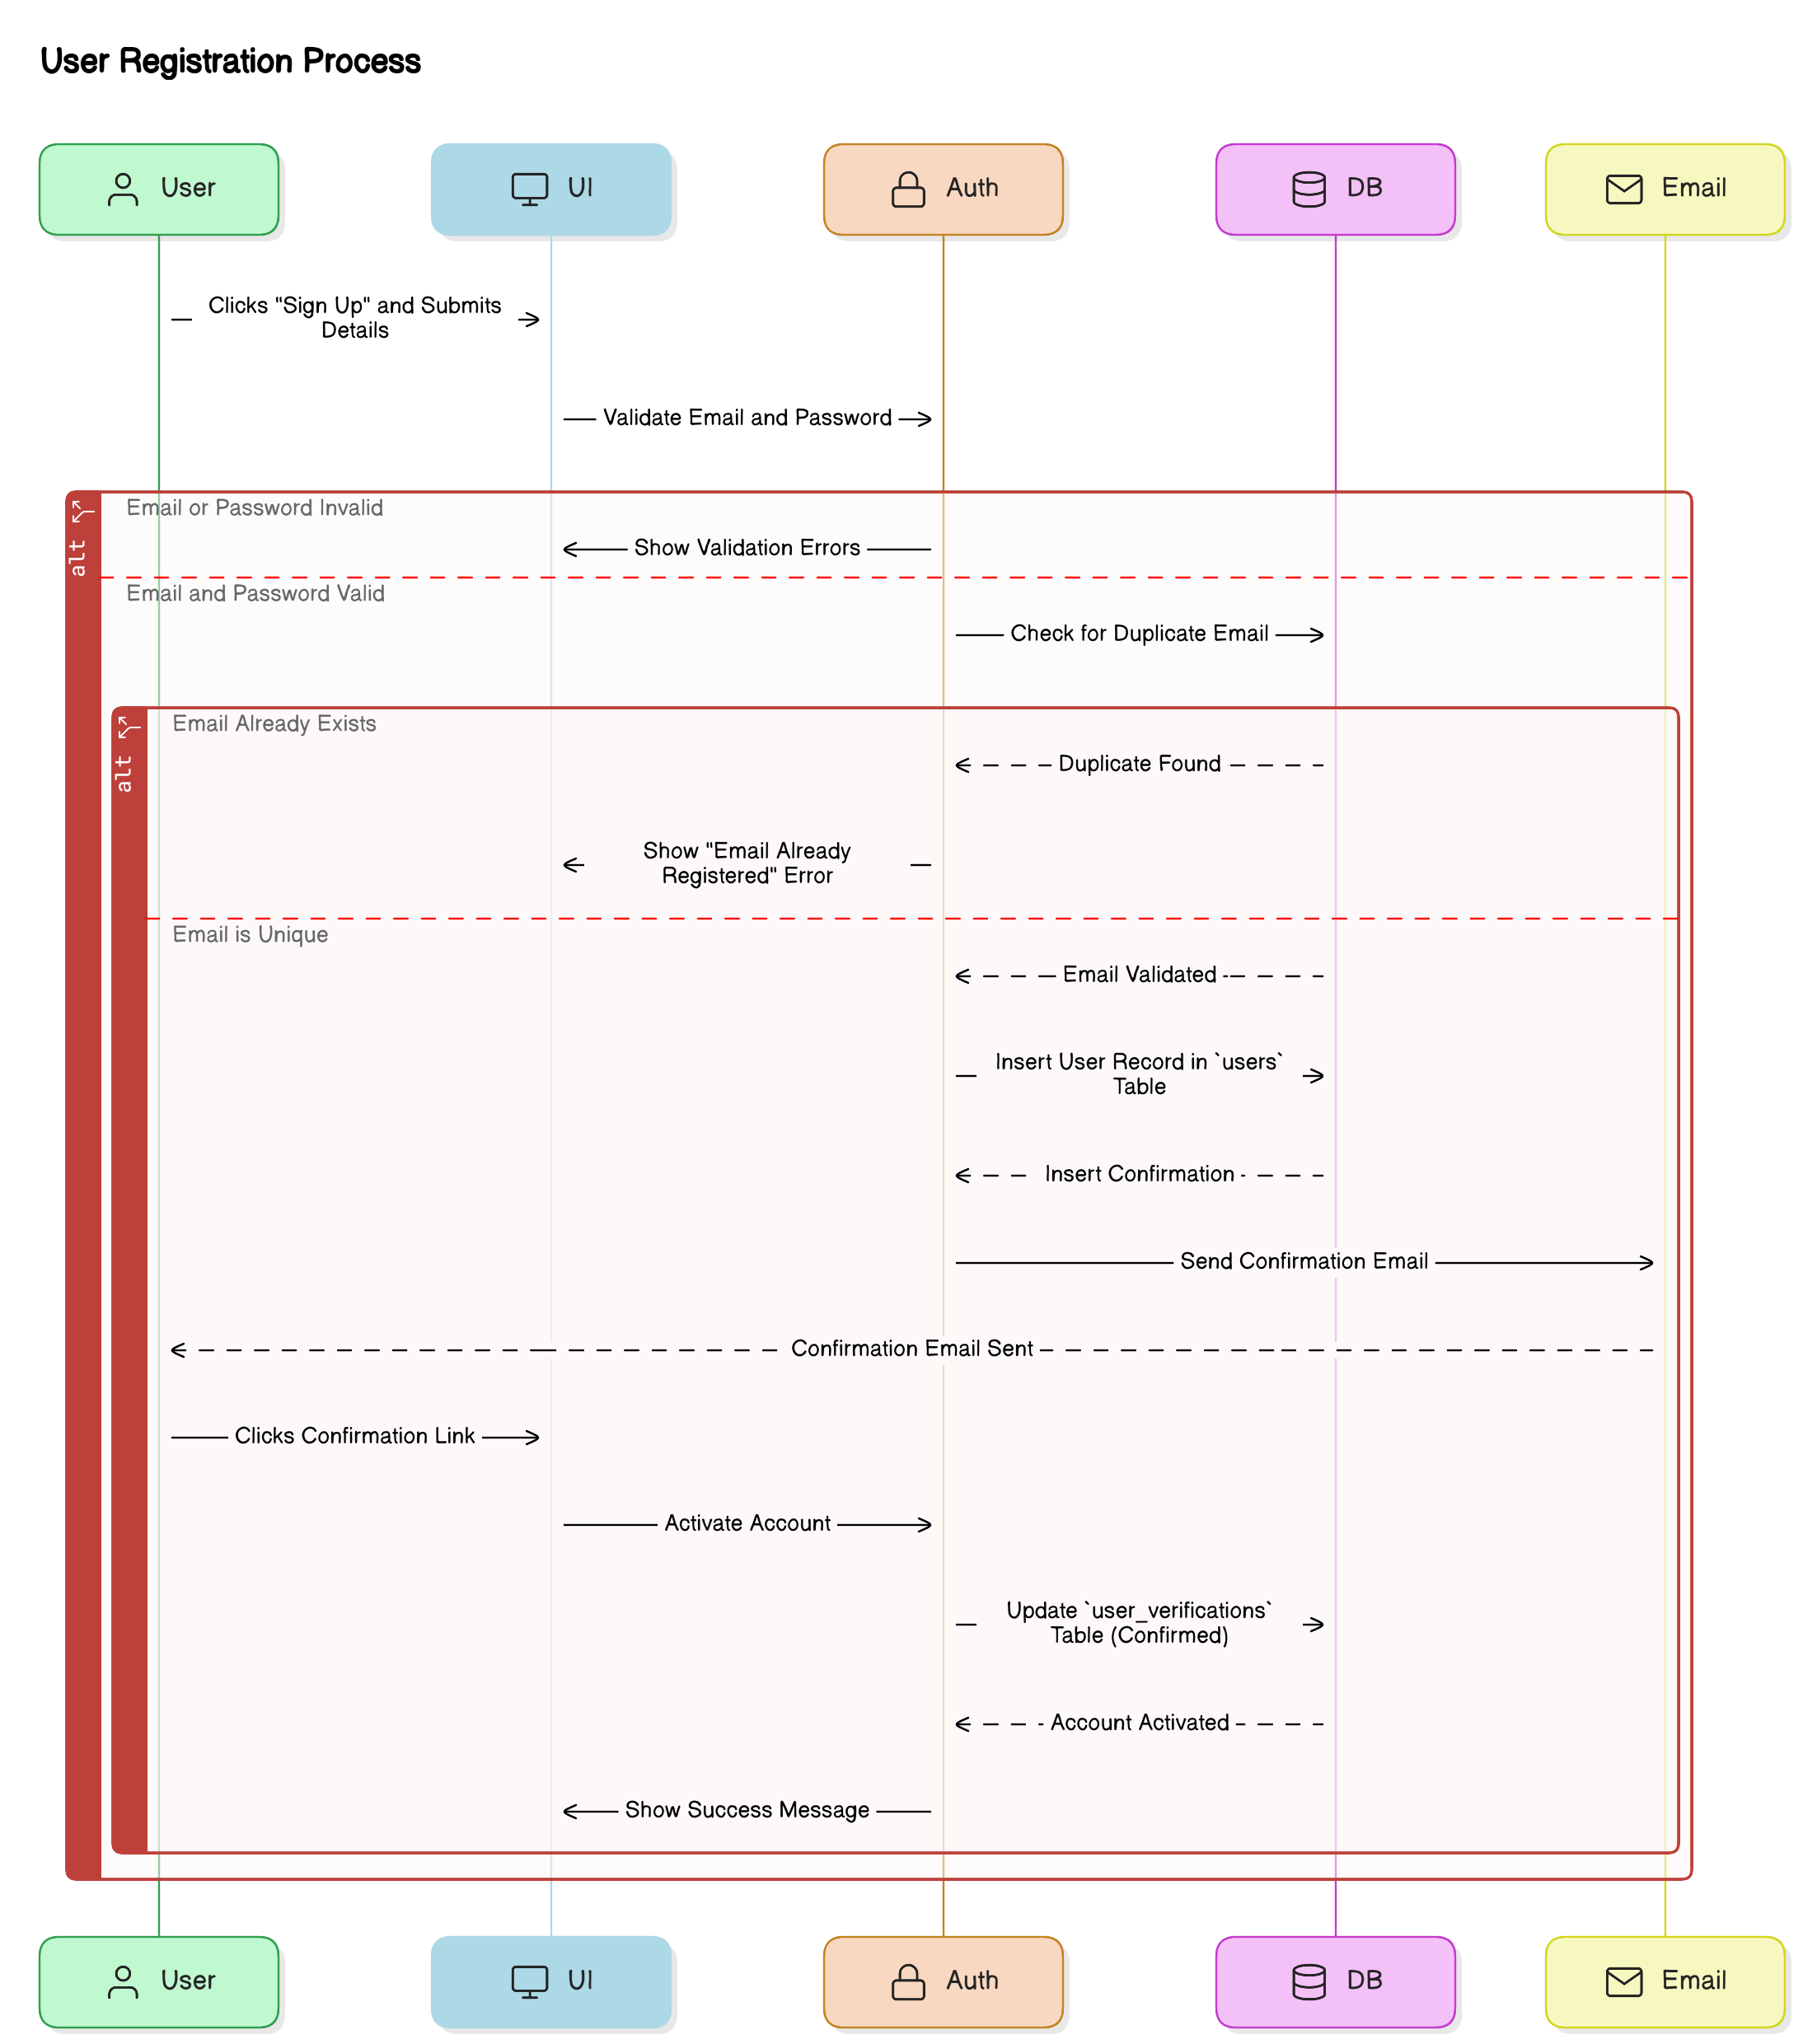
\includegraphics[width=0.9\textwidth]{images/sequence_diagrams/user_registration_process.png}
    \caption{User registration sequence diagram}
    \label{fig:user_registration}
\end{figure}

\subsection{User Login Process}
\begin{figure}[H]
    \centering
    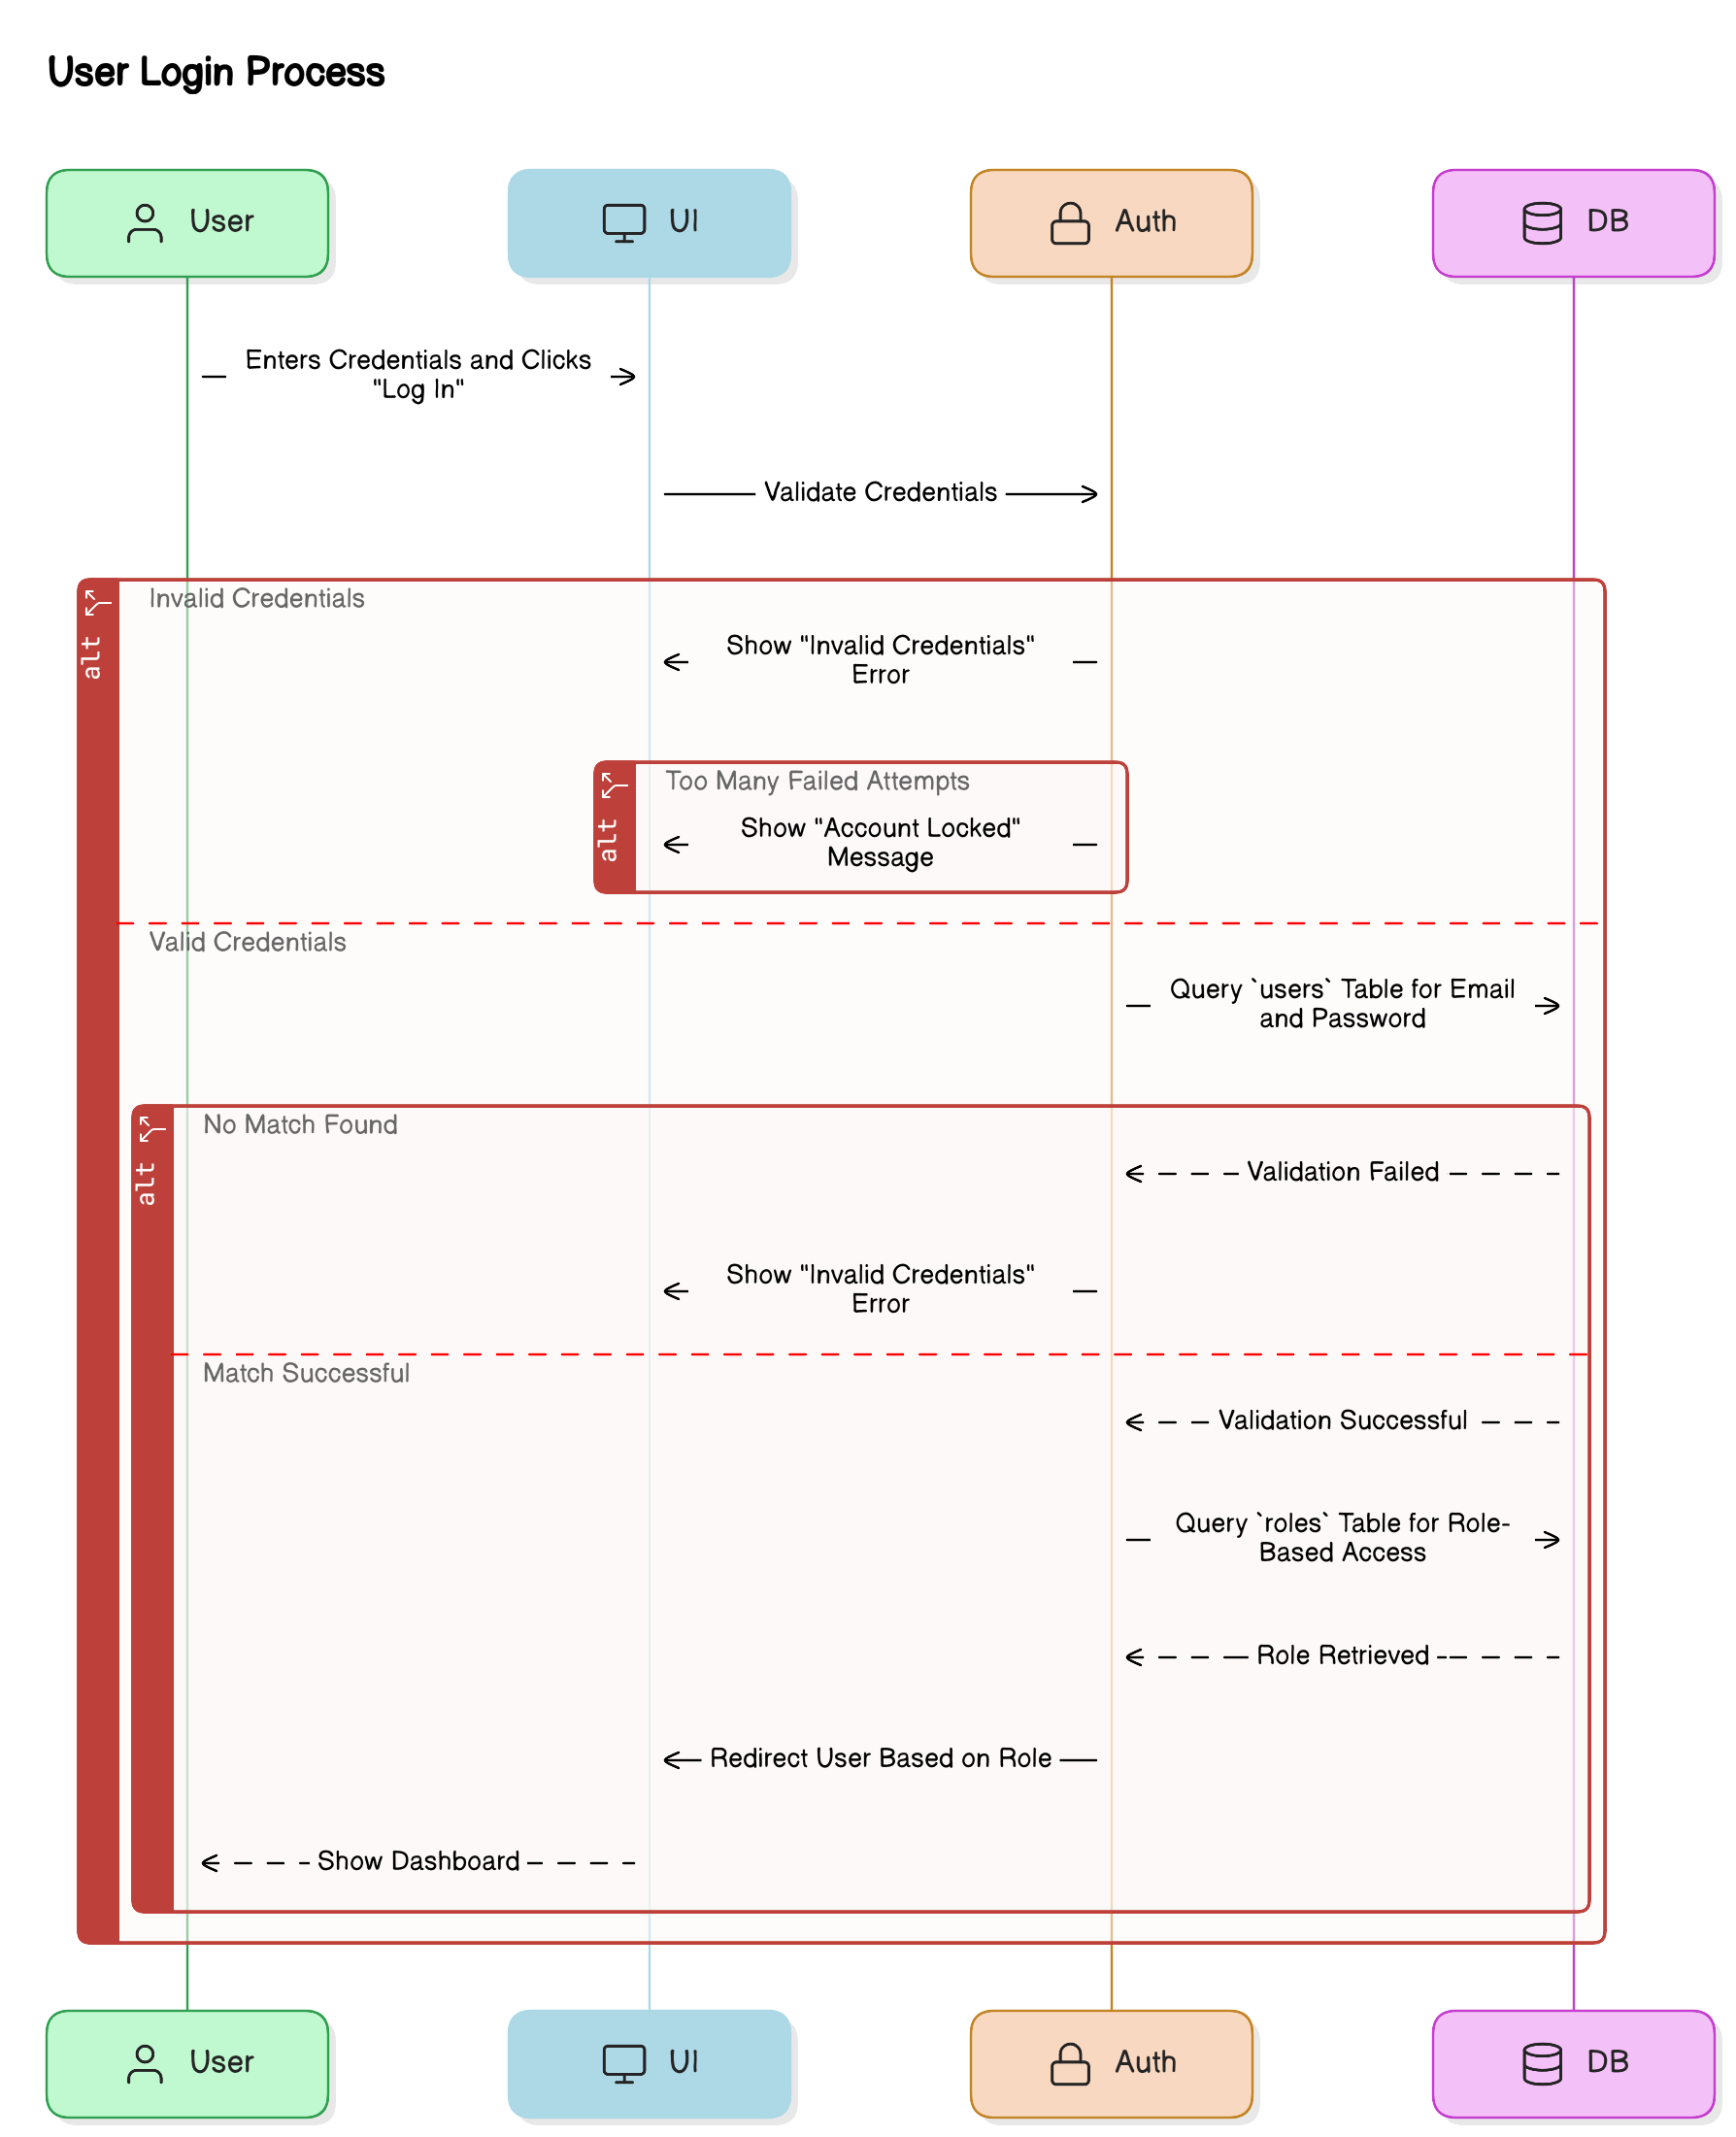
\includegraphics[width=0.9\textwidth]{images/sequence_diagrams/user_login_process.png}
    \caption{Authentication sequence with security measures}
    \label{fig:user_login}
\end{figure}

\subsection{Password Recovery Process}
\begin{figure}[H]
    \centering
    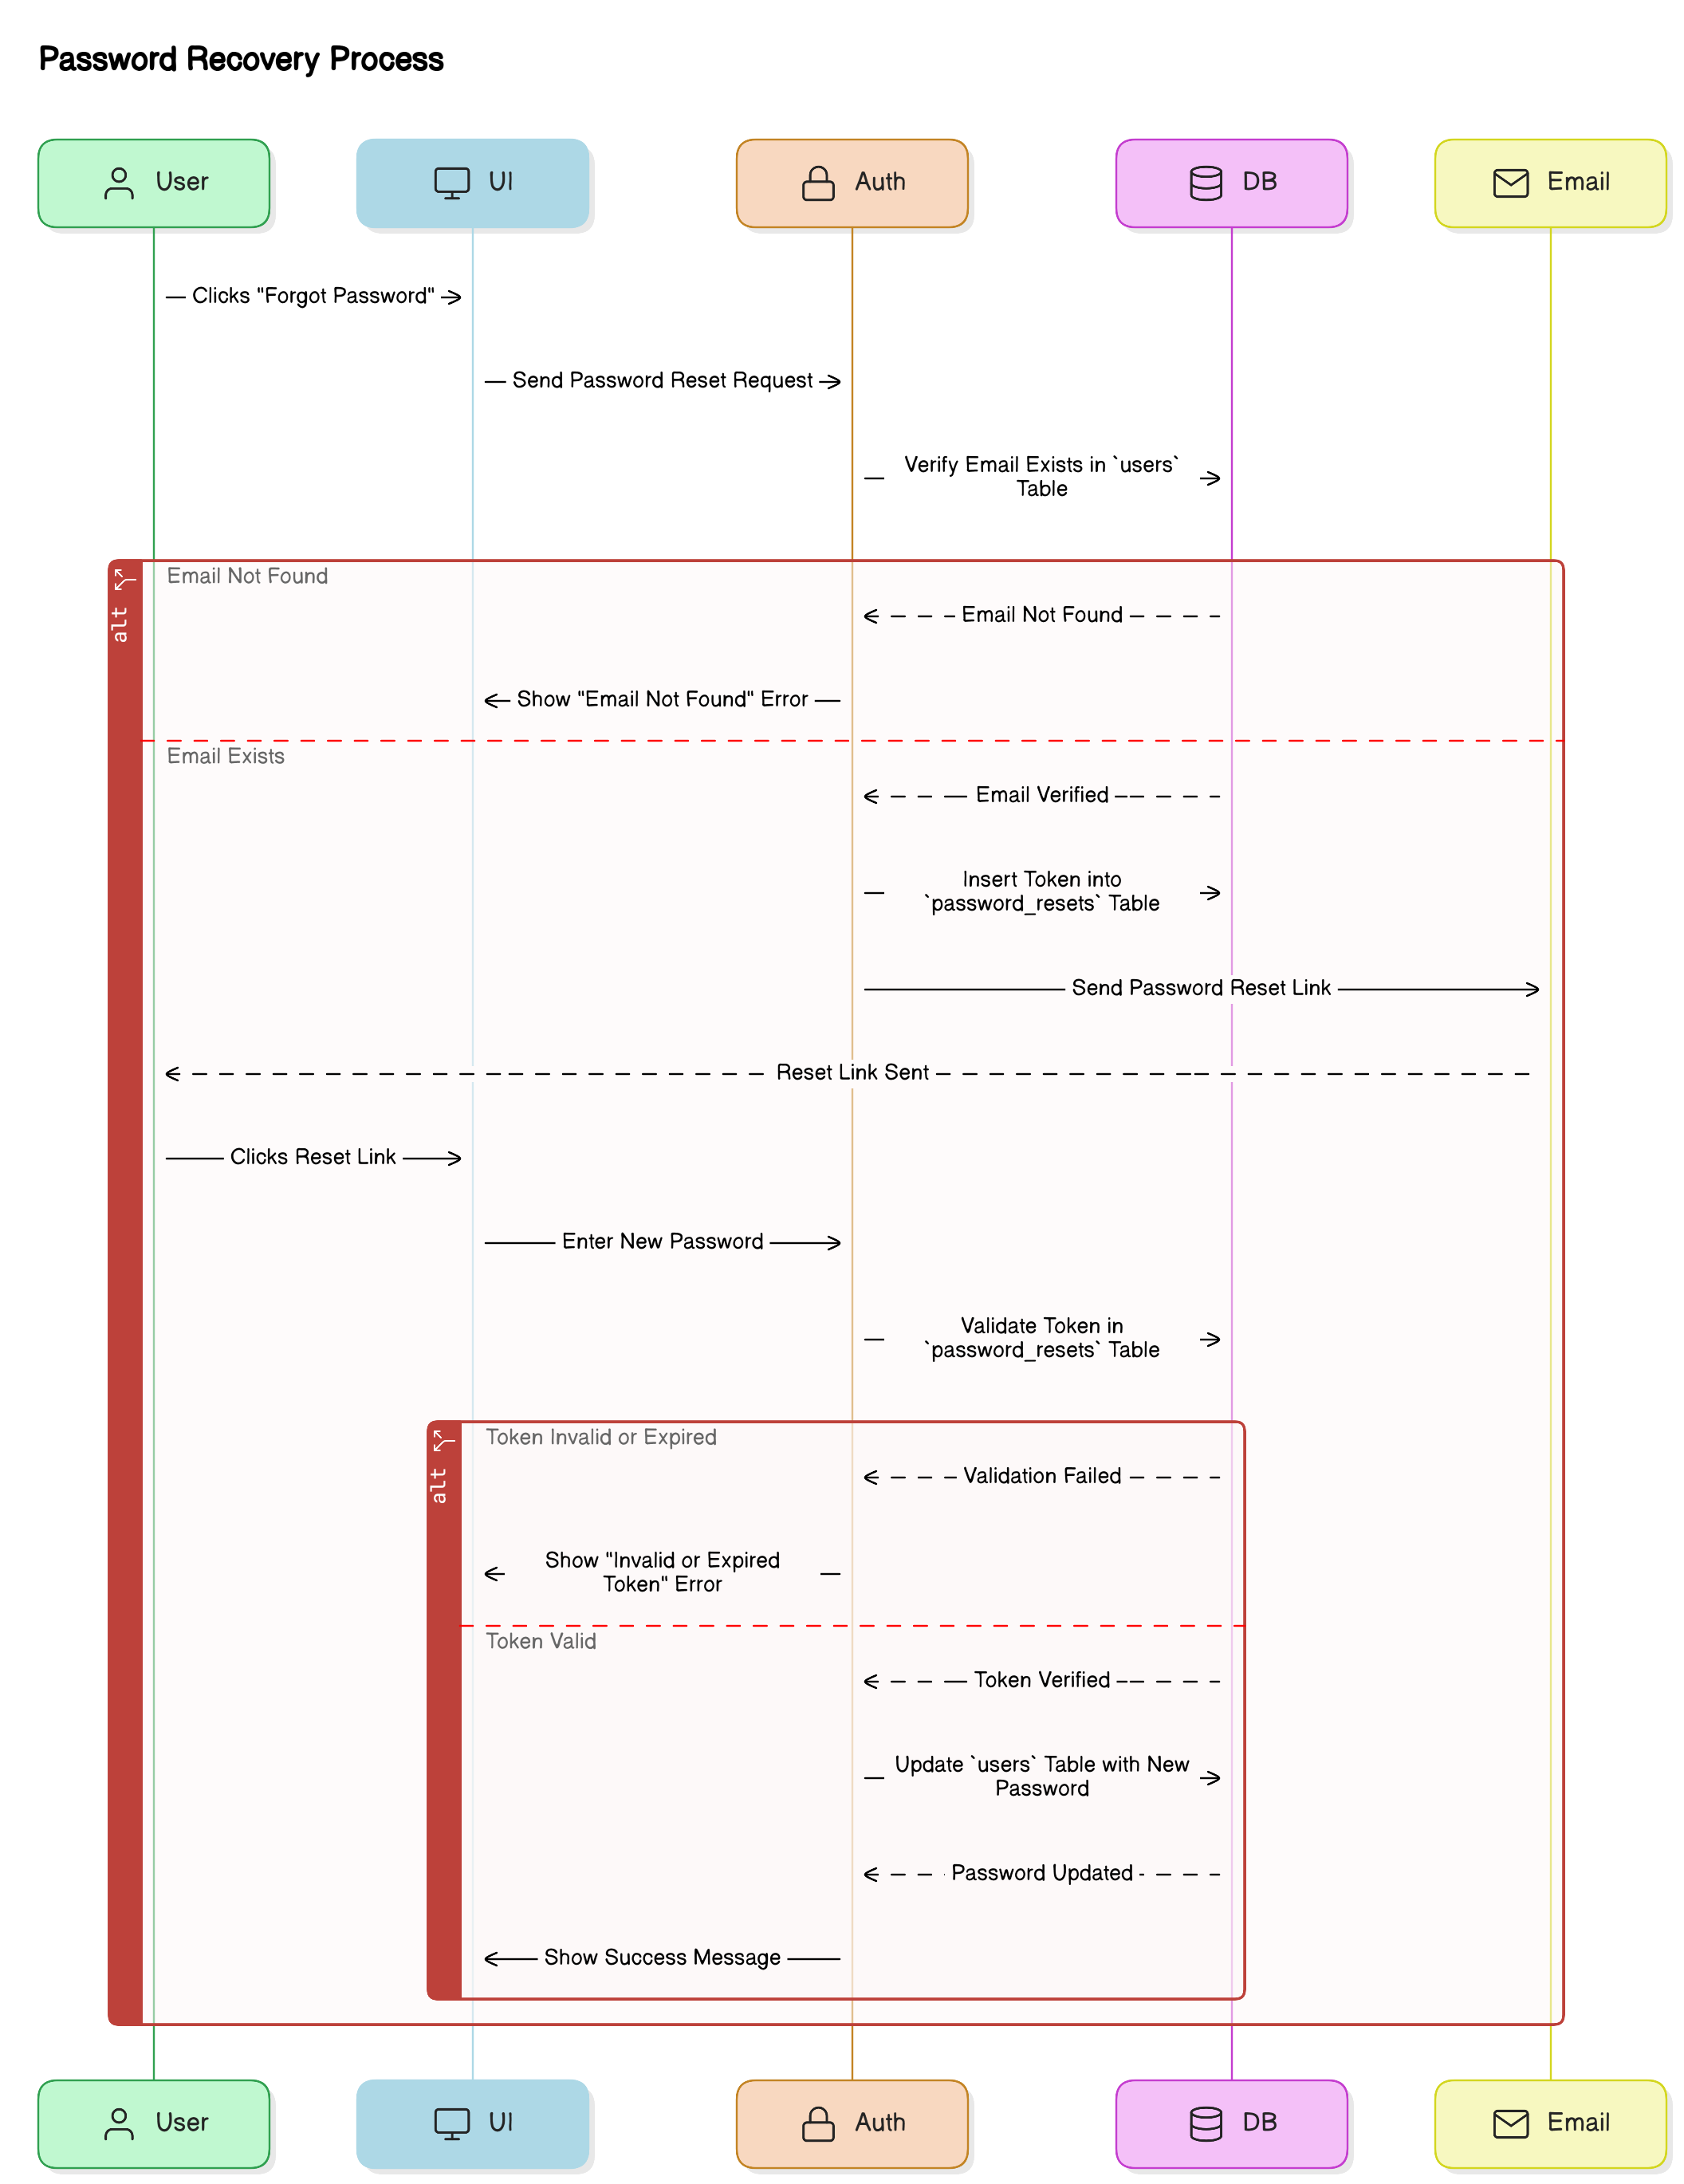
\includegraphics[width=0.9\textwidth]{images/sequence_diagrams/password_recovery_process.png}
    \caption{Password reset sequence diagram with email verification}
    \label{fig:password_recovery}
\end{figure}

\subsection{Create Profile Process}
\begin{figure}[H]
    \centering
    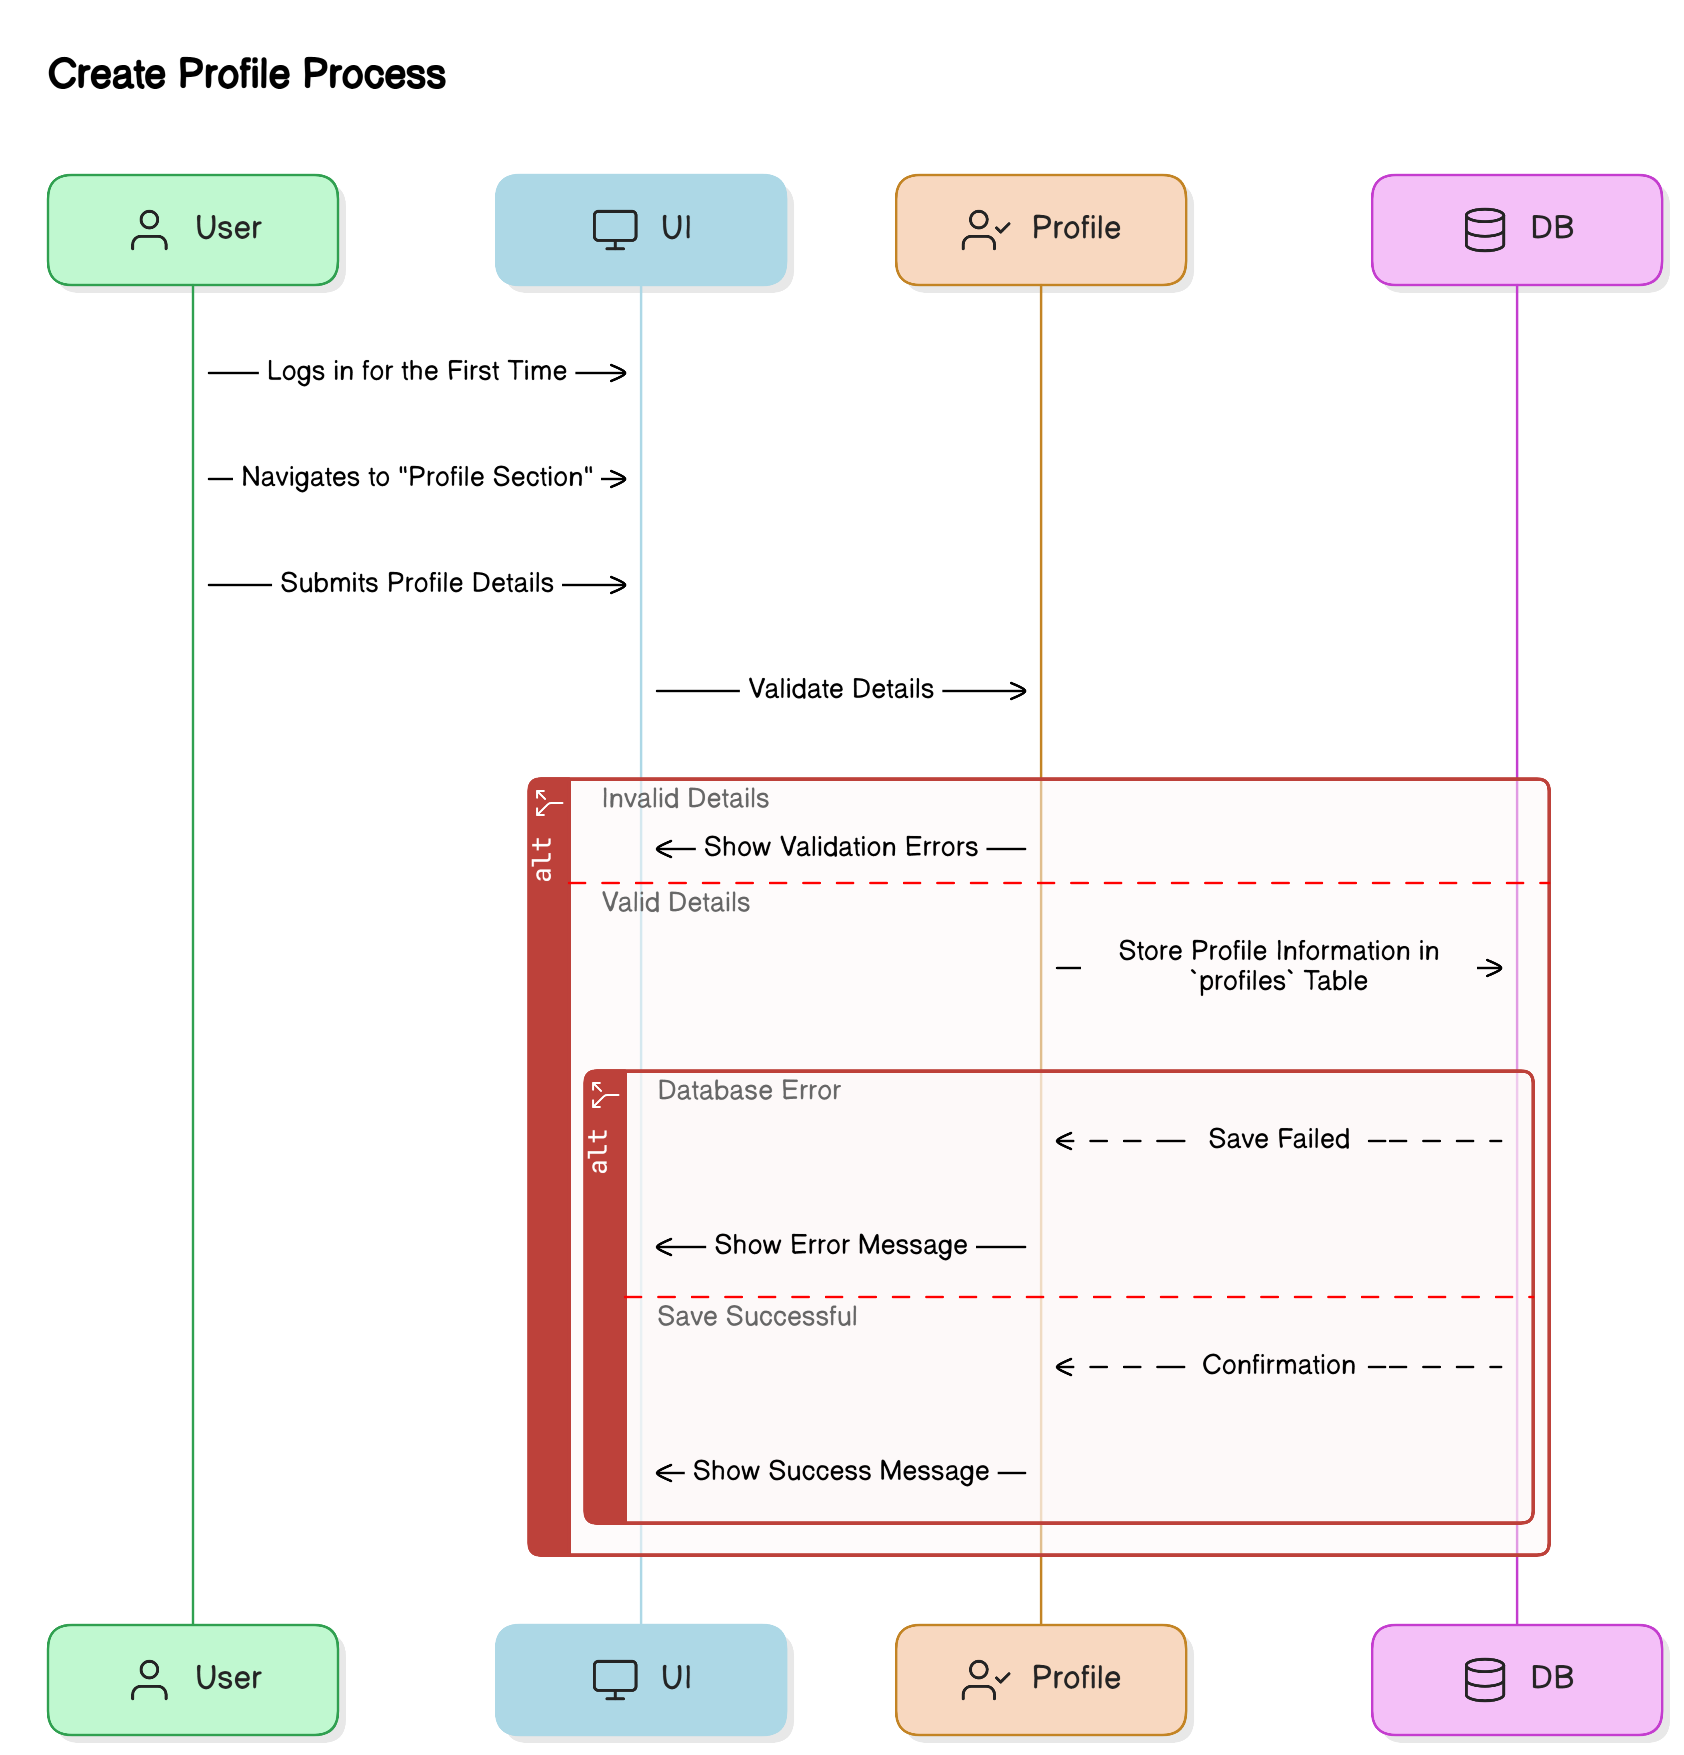
\includegraphics[width=0.9\textwidth]{images/sequence_diagrams/create_profile_process.png}
    \caption{Profile creation sequence diagram showing validation and database storage}
    \label{fig:create_profile}
\end{figure}

\subsection{Create Group Process}
\begin{figure}[H]
    \centering
    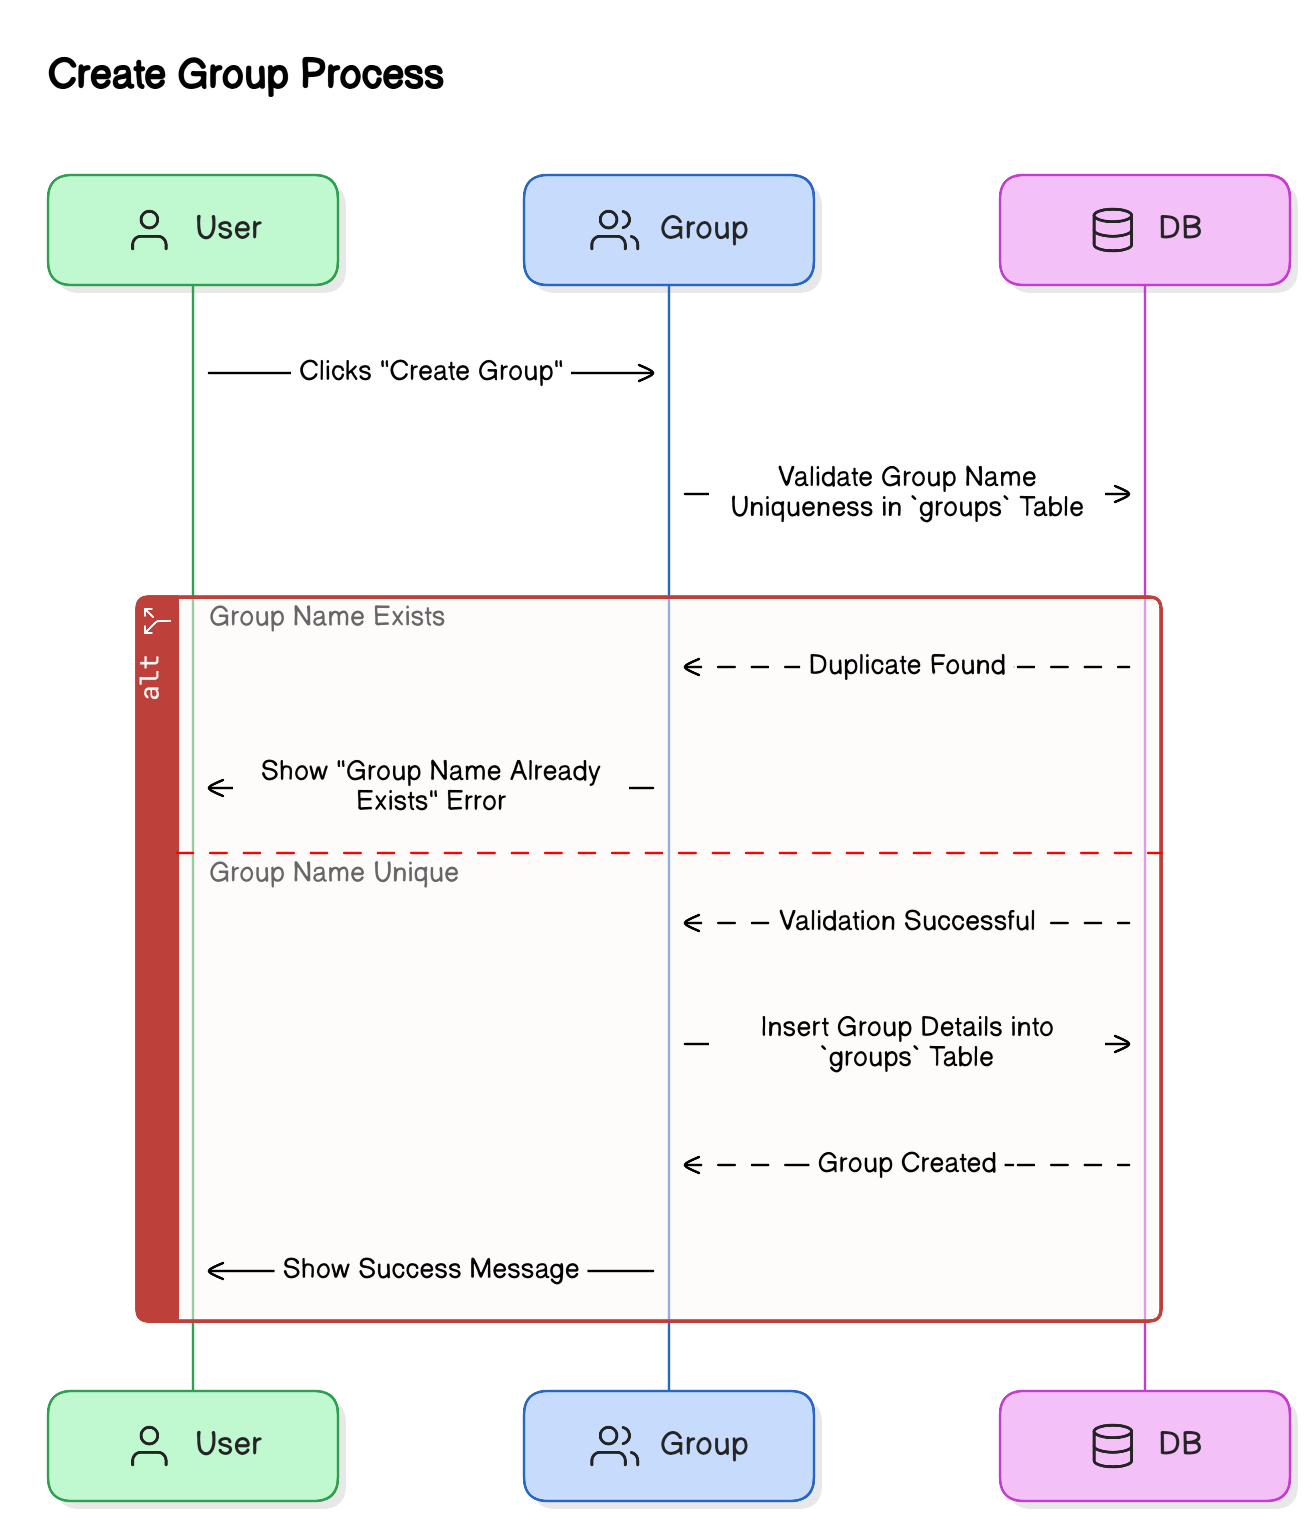
\includegraphics[width=0.9\textwidth]{images/sequence_diagrams/create_group_process.png}
    \caption{Group creation sequence diagram}
    \label{fig:create_group}
\end{figure}

\subsection{Direct Messaging Process}
\begin{figure}[H]
    \centering
    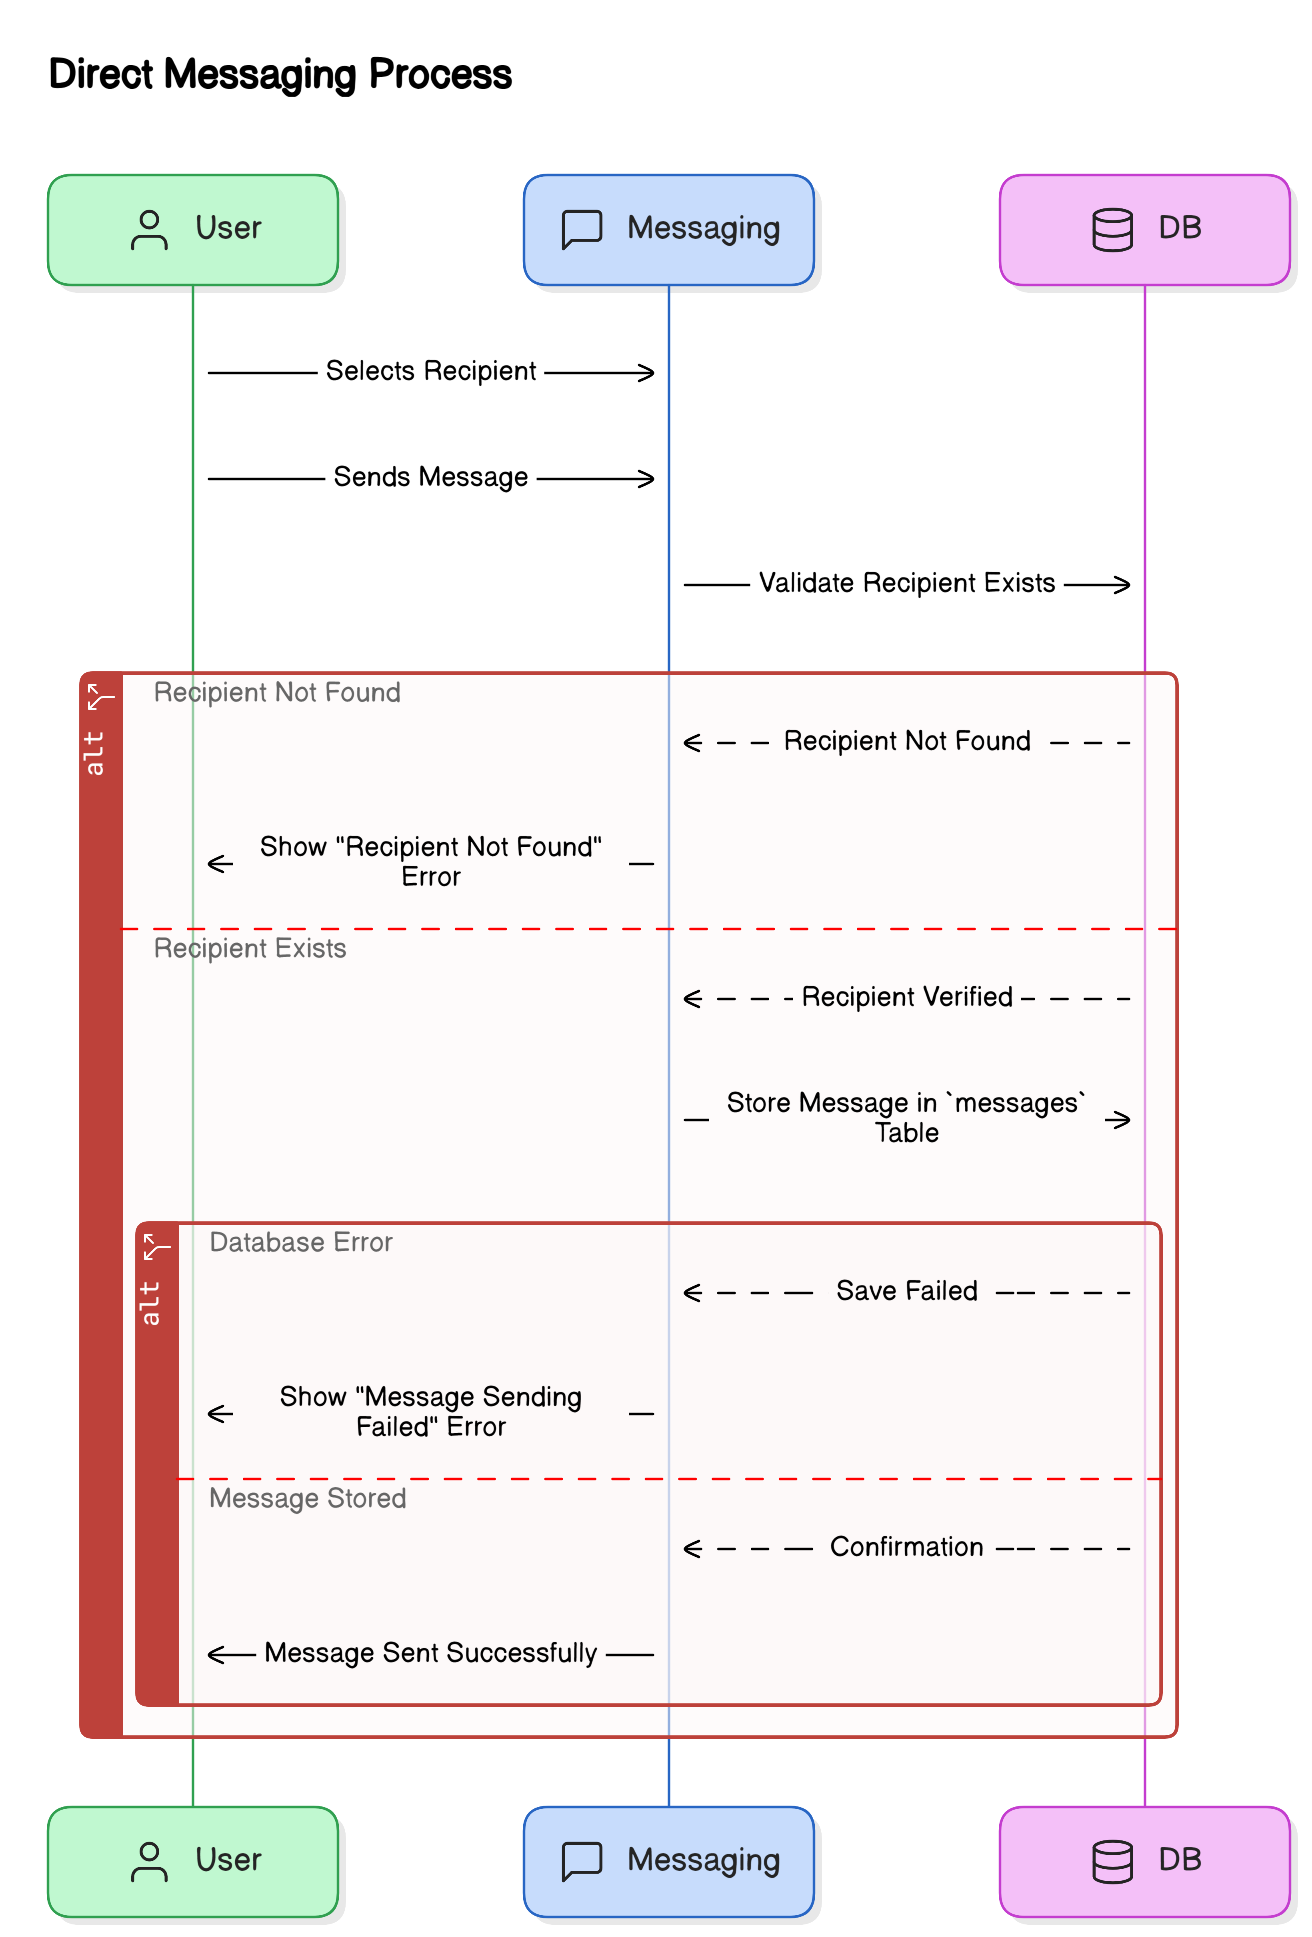
\includegraphics[width=0.9\textwidth]{images/sequence_diagrams/direct_messaging_process.png}
    \caption{Messaging sequence diagram}
    \label{fig:messaging}
\end{figure}

\subsection{Start a Discussion Process}
\begin{figure}[H]
    \centering
    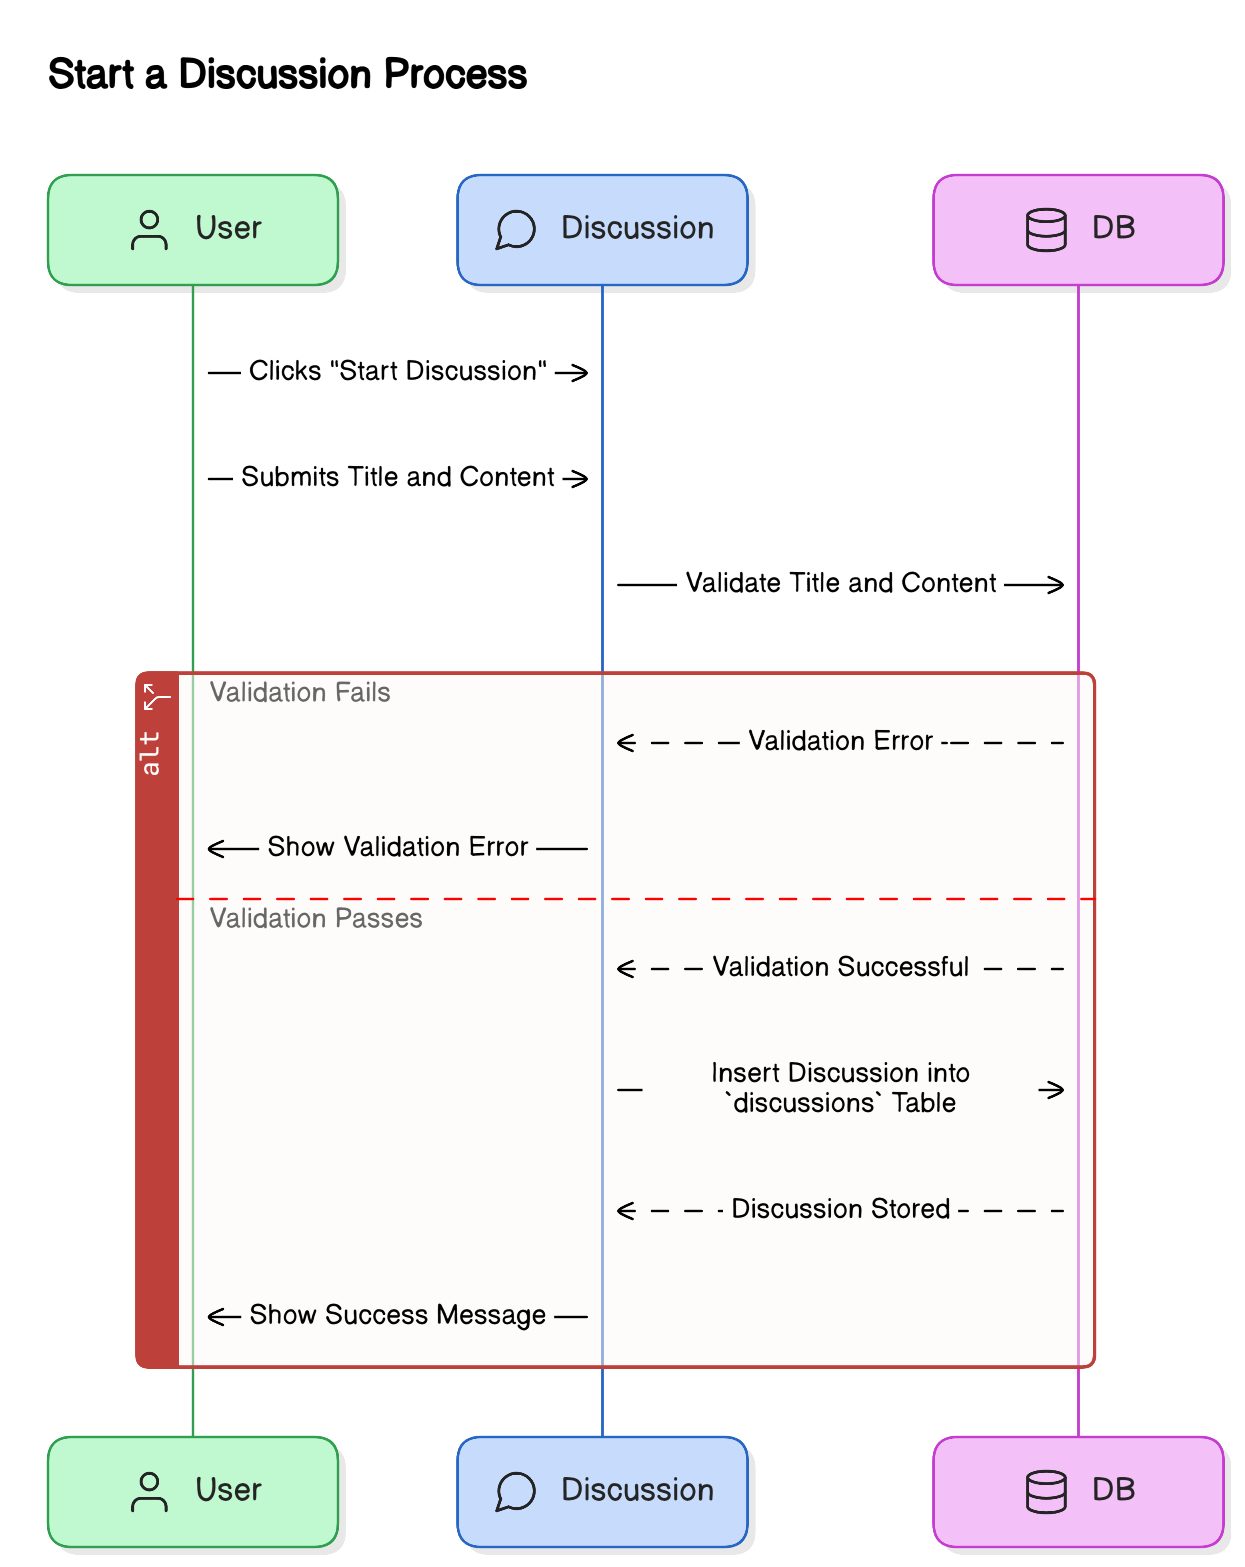
\includegraphics[width=0.9\textwidth]{images/sequence_diagrams/start_a_discussion_process.png}
    \caption{Group discussion initiation sequence}
    \label{fig:start_discussion}
\end{figure}

\subsection{Upload Academic Material Process}
\begin{figure}[H]
    \centering
    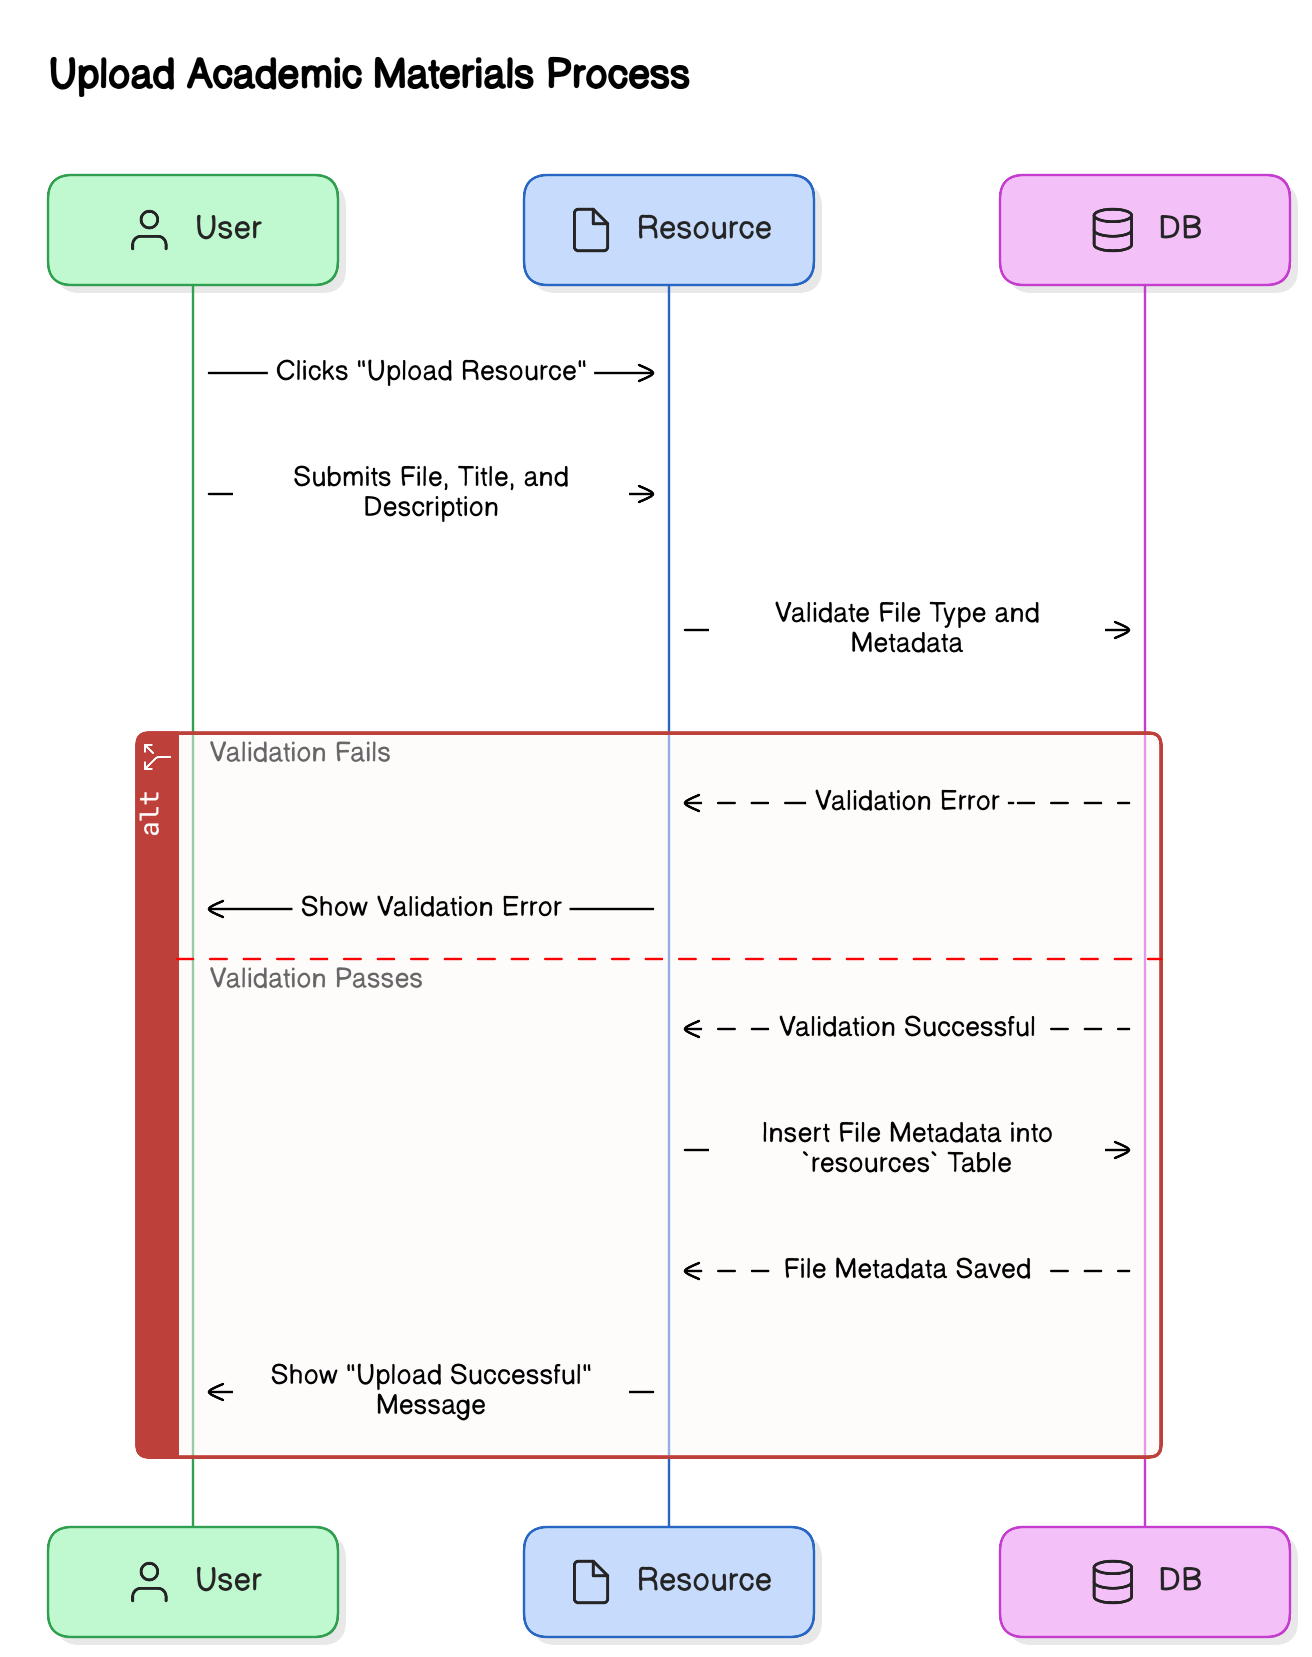
\includegraphics[width=0.9\textwidth]{images/sequence_diagrams/upload_academic_material_process.png}
    \caption{Resource upload sequence with file validation}
    \label{fig:upload_material}
\end{figure}

\subsection{Create Event Process}
\begin{figure}[H]
    \centering
    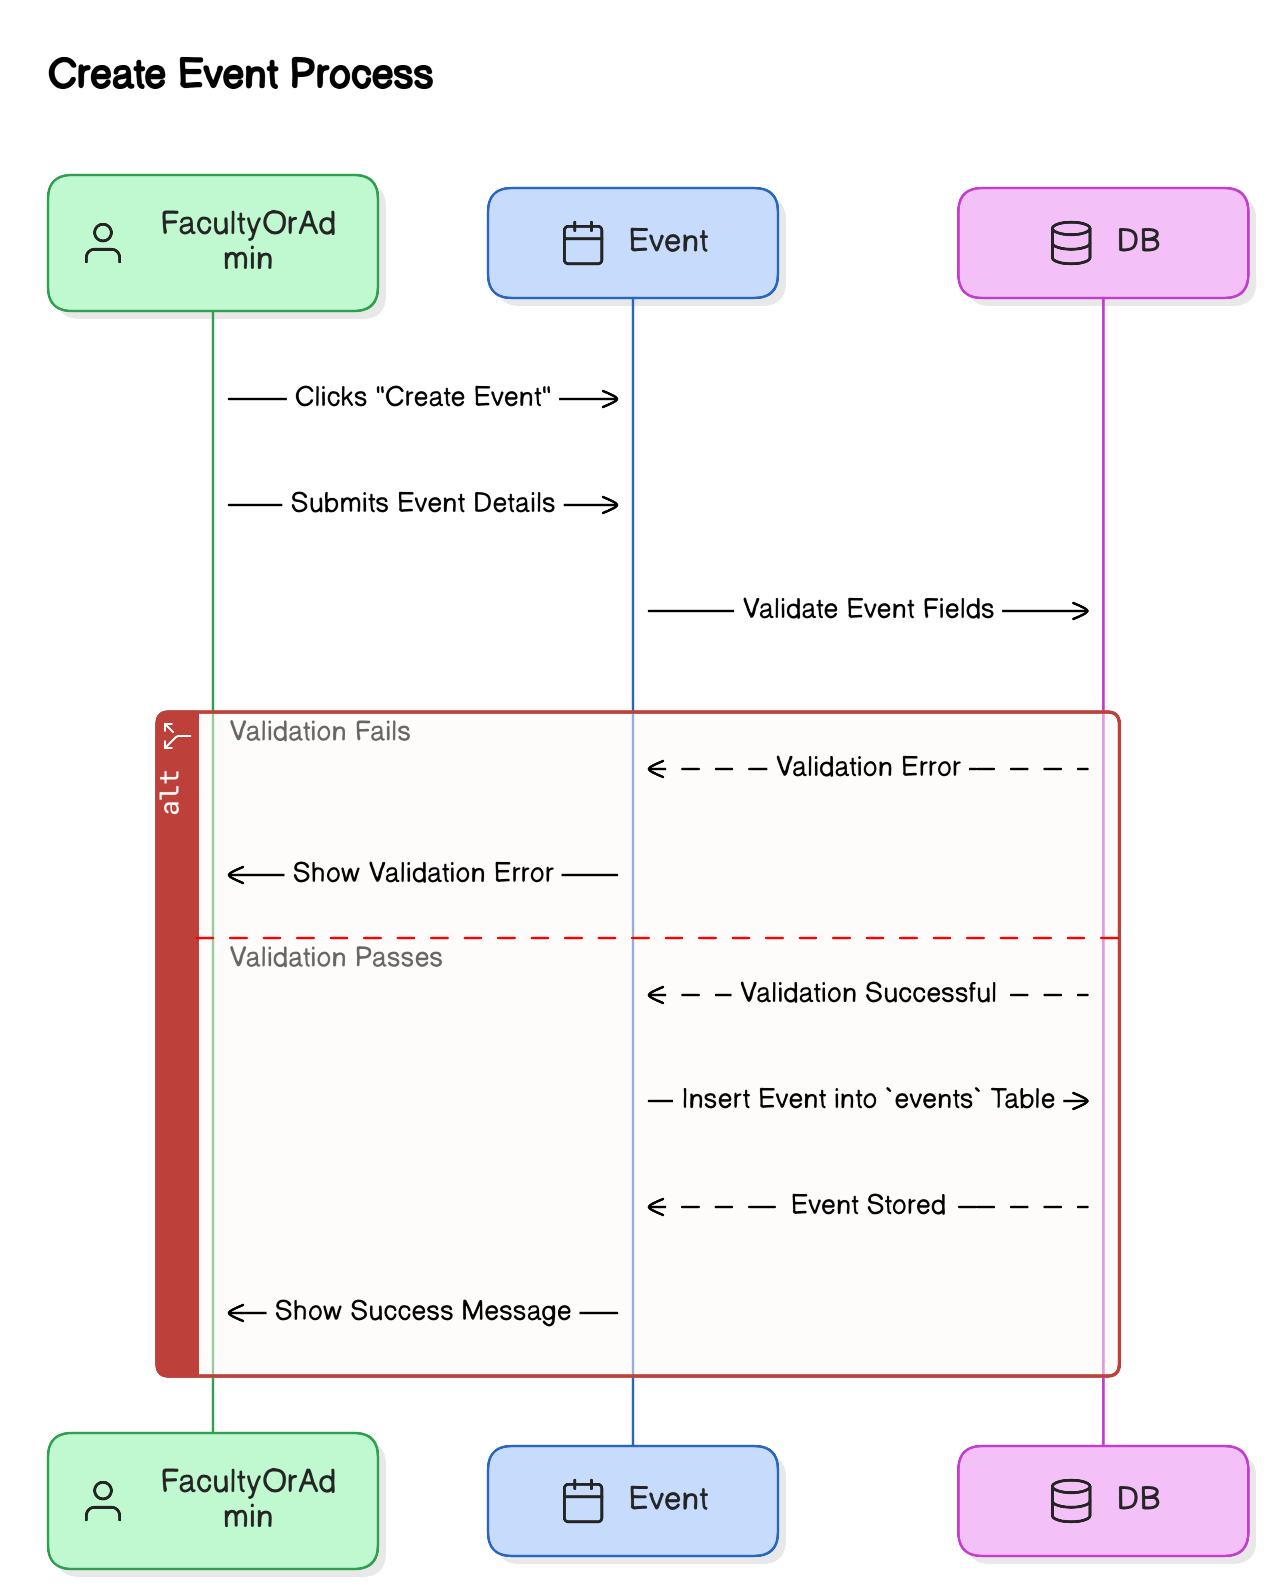
\includegraphics[width=0.9\textwidth]{images/sequence_diagrams/create_event_process.png}
    \caption{Event creation workflow for faculty/admins}
    \label{fig:create_event}
\end{figure}

\vspace{3cm}

\section{Class Diagram}
The class diagram represents the core domain model of the Student Portal system:

\begin{figure}[H]
    \centering
    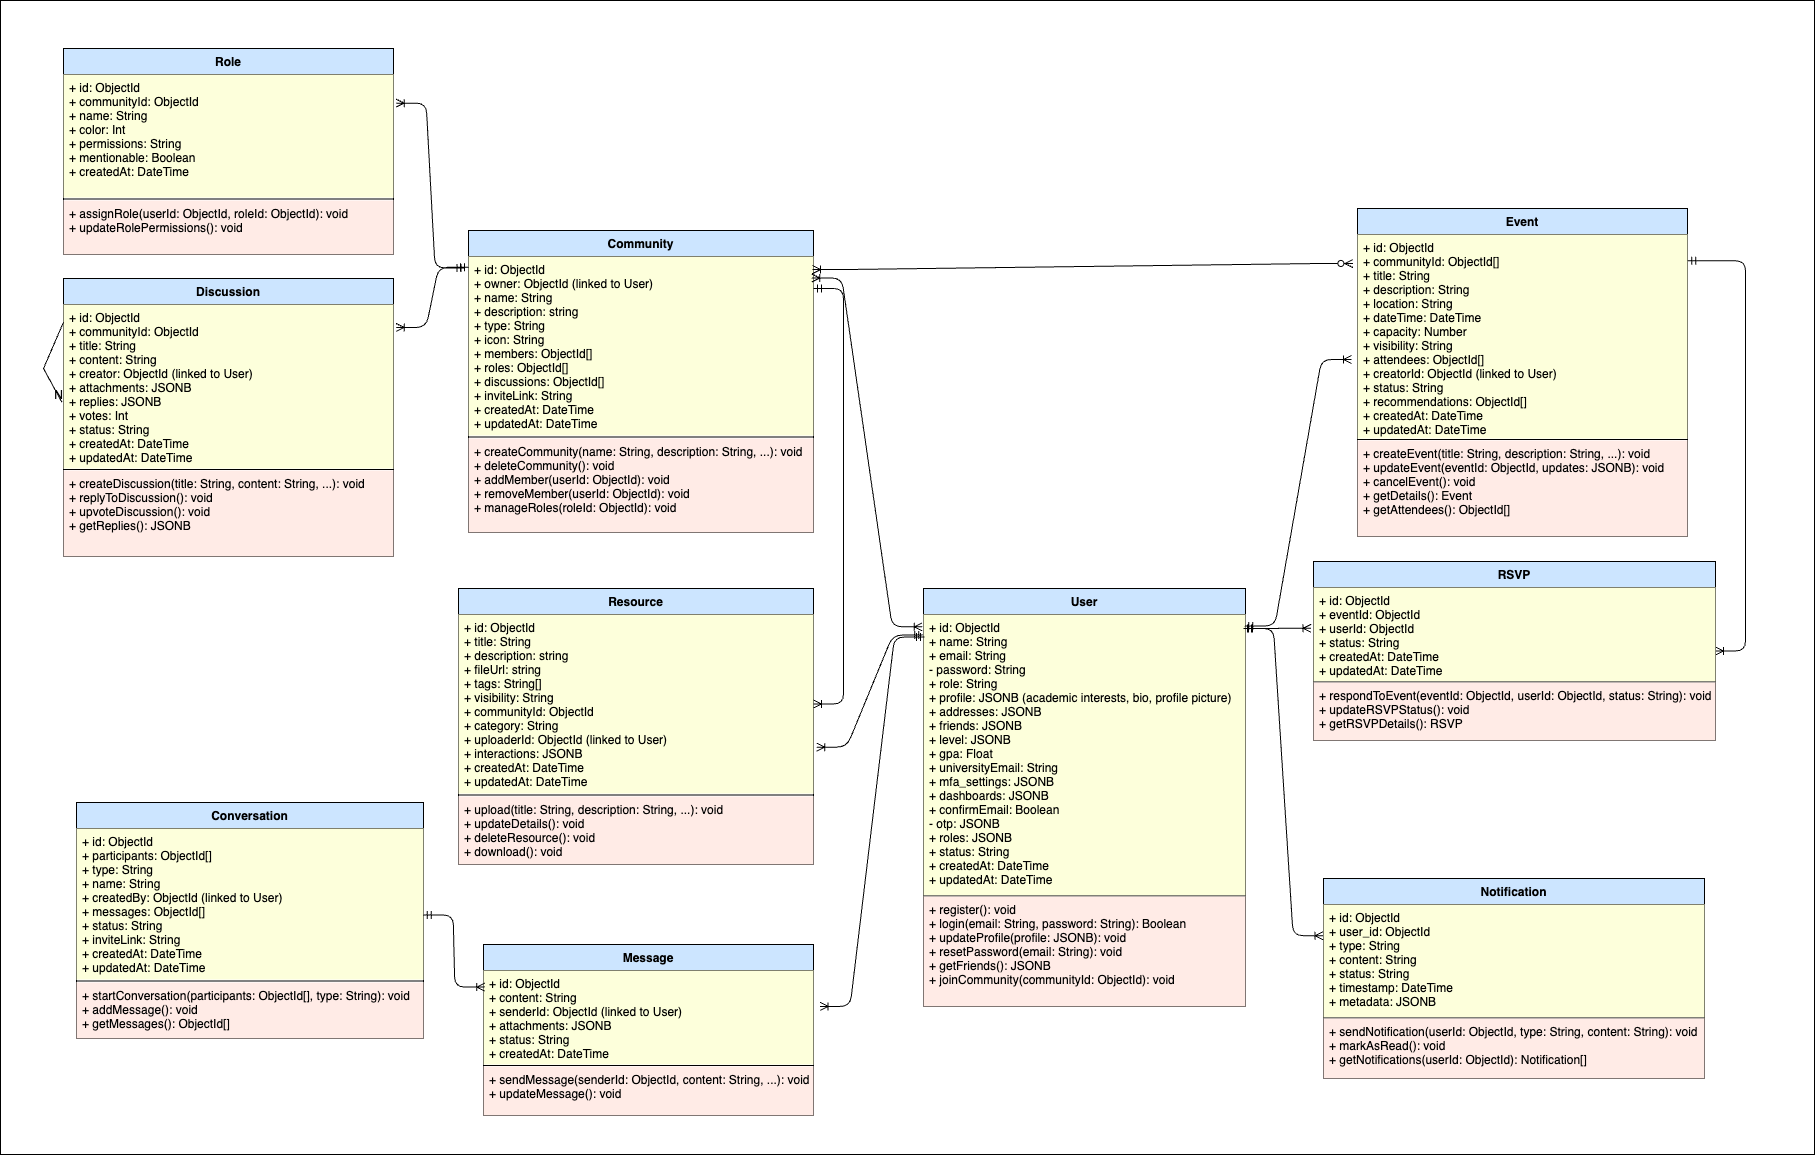
\includegraphics[width=\textwidth]{images/uml.png} 
    \caption{Class diagram of the Student Portal system}
    \label{fig:class_diagram}
\end{figure}

\section{Entity Relationship Diagram (ERD)}
\begin{adjustbox}{width=\textwidth, height=0.35\textheight, keepaspectratio, center}
    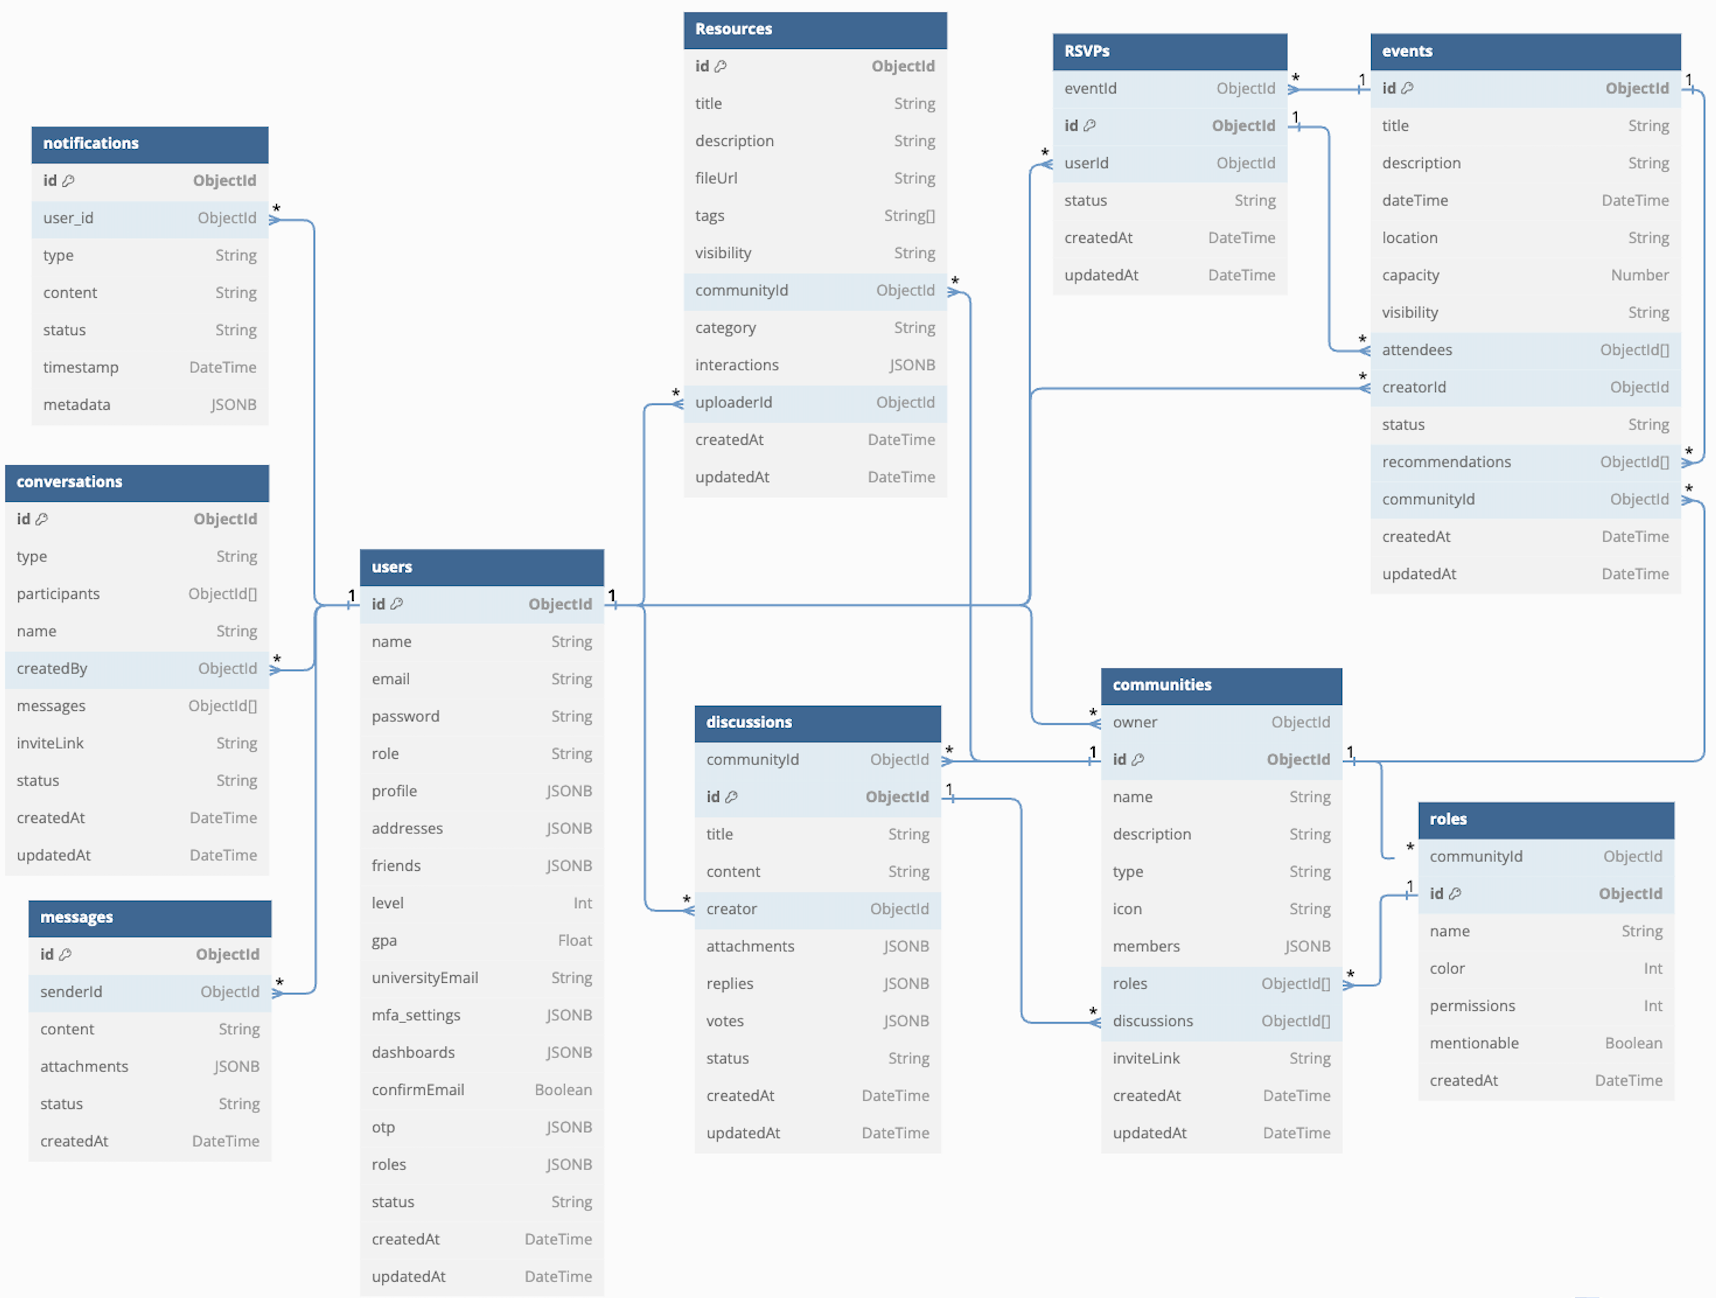
\includegraphics{images/schema_diagram.png}
\end{adjustbox}



\section{Data Dictionary}

\subsection{Users Table}
\begin{longtable}{|L{3cm}|C{2cm}|L{2.5cm}|L{3cm}|L{3cm}|}
\hline
\textbf{Field} & \textbf{Type} & \textbf{Description} & \textbf{Constraints} & \textbf{Example} \\ \hline
\endhead

id & ObjectId & Unique user identifier & Primary key, auto-generated & 507f1f77bc-f86cd799439011 \\ \hline
name & String & Full name of the user & Required, max 255 chars & John Doe \\ \hline
email & String & Login credential & Unique, required & john.doe@ example.com \\ \hline
password & String & Encrypted password & Bcrypt hashed & hashed\_password \\ \hline
role & String & Access level & Enum: Student/Faculty/Admin & Student \\ \hline
profile & JSONB & User profile data & Optional & \{bio:CS Student\} \\ \hline
status & String & Online status & Enum: online/offline/ idle/dnd & online \\ \hline
createdAt & DateTime & Account creation time & Auto-generated & 2023-07-01T12:00:00Z \\ \hline

\caption{Users table data dictionary}
\label{tab:users_dict}
\end{longtable}

\subsection{Communities Table}
\begin{longtable}{|L{3cm}|C{2cm}|L{2.5cm}|L{3cm}|L{3cm}|}
\hline
\textbf{Field} & \textbf{Type} & \textbf{Description} & \textbf{Constraints} & \textbf{Example} \\ \hline
\endhead

id & ObjectId & Group identifier & Primary key, auto-generated & 507f1f77bc-f86cd799439200 \\ \hline
name & String & Community name & Unique, required & AI Enthusiasts \\ \hline
type & String & Group classification & Enum: official/community & official \\ \hline
owner & ObjectId & Creator reference & Foreign key to users & 507f1f77bc-f86cd799439100 \\ \hline
members & JSONB & Member list & Array of user objects & \{userId:507...\} \\ \hline
createdAt & DateTime & Creation timestamp & Auto-generated & 2024-01-10T08:45:00Z \\ \hline

\caption{Communities table data dictionary}
\label{tab:communities_dict}
\end{longtable}

\subsection{Embedded Structures}

\begin{longtable}{|C{3.5cm}|C{2cm}|C{4cm}|C{3cm}|}
\hline
\textbf{Field} & \textbf{Type} & \textbf{Description} & \textbf{Example} \\ \hline
\endhead

members.userId & ObjectId & Member reference & 507f1f77bcf 86cd799439101 \\ \hline
members.roleIds & ObjectId[] & Assigned roles & ["507f1f77bcf8 6cd799439300"] \\ \hline
members.joinedAt & DateTime & Join timestamp & 2024-01-10T09:30:00Z \\ \hline

\caption{Embedded members structure}
\label{tab:members_struct}
\end{longtable}

\subsection{Discussions Table}
\begin{longtable}{|L{3cm}|C{2cm}|L{2.5cm}|L{3cm}|L{3cm}|}
\hline
\textbf{Field} & \textbf{Type} & \textbf{Description} & \textbf{Constraints} & \textbf{Example} \\ \hline
\endhead

id & ObjectId & Discussion identifier & Primary key & 507f1f77bcf8 6cd799439200 \\ \hline
communityId & ObjectId & Parent community & Foreign key & 507f1f77b cf86cd799439100 \\ \hline
title & String & Discussion title & Required, max 255 chars & "Best Practices for Web Dev" \\ \hline
content & String & Main content & Required & "What are the best practices?"  \hline
creator & ObjectId & Author reference & Foreign key to users & 507f1f77bcf 86cd799439101 \hline
status & String & Discussion state & Enum: open/closed/archived & "open" \\ \hline
createdAt & DateTime & Creation time & Auto-generated & 2024-01-10T08: 45:00Z \hline
\caption{Discussions table data dictionary}
\label{tab:discussions_dict}
\end{longtable}

\subsection{Conversations Table}
\begin{longtable}{|L{3cm}|C{2cm}|L{2.5cm}|L{3cm}|L{3cm}|}
\hline
\textbf{Field} & \textbf{Type} & \textbf{Description} & \textbf{Constraints} & \textbf{Example} \\ \hline
\endhead

id & ObjectId & Conversation ID & Primary key & 507f1f77bcf 86cd799439100 \\ \hline
type & String & Conversation type & Enum: DM/GroupDM & "GroupDM" \\ \hline
participants & ObjectId[] & Participant list & Min 2 for GroupDM & ["507...101", "507...102"] \\ \hline
createdBy & ObjectId & Creator reference & Foreign key to users & 507f1f77bc f86cd799439103 \\ \hline
status & String & Conversation state & Enum: active/archived & "active" \\ \hline

\caption{Conversations table data dictionary}
\label{tab:conversations_dict}
\end{longtable}

\subsection{Messages Table}
\begin{longtable}{|L{3cm}|C{2cm}|L{2.5cm}|L{3cm}|L{3cm}|}
\hline
\textbf{Field} & \textbf{Type} & \textbf{Description} & \textbf{Constraints} & \textbf{Example} \\ \hline
\endhead

id & ObjectId & Message identifier & Primary key & 60d21b4667d 0d8992e610c85 \\ \hline
senderId & ObjectId & Sender reference & Foreign key to users & 60d21b4667d 0d8992e610c90 \\ \hline
content & String & Message text & Optional & "Hello, how are you?" \\ \hline
status & String & Delivery status & Enum: sent/ delivered/read & "delivered" \\ \hline
createdAt & DateTime & Send timestamp & Auto-generated & 2024-01-28T12:00:00Z \\ \hline

\caption{Messages table data dictionary}
\label{tab:messages_dict}
\end{longtable}

\subsection{Embedded Structures}

\subsubsection{Discussion Attachments}
\begin{longtable}{|C{2.5cm}|C{1.8cm}|C{4cm}|C{4cm}|}
\hline
\textbf{Field} & \textbf{Type} & \textbf{Description} & \textbf{Example} \\ \hline
\endhead

type & String & Attachment type & "file" \\ \hline
resource & String & Resource URL & "https://files.com/ doc.pdf" \\ \hline

\caption{Discussion attachments structure}
\label{tab:discussion_attachments}
\end{longtable}

\subsubsection{Discussion Replies}
\begin{longtable}{|C{2.5cm}|C{1.8cm}|C{4cm}|C{3cm}|}
\hline
\textbf{Field} & \textbf{Type} & \textbf{Description} & \textbf{Example} \\ \hline
\endhead

id & ObjectId & Reply identifier & 507f1f77bc f86cd799439300 \\ \hline
content & String & Reply content & "I agree!" \\ \hline
creator & ObjectId & Author reference & 507f1f77bc f86cd799439102 \\ \hline
createdAt & DateTime & Creation time & 2024-01-11T09:00:00Z \\ \hline

\caption{Discussion replies structure}
\label{tab:discussion_replies}
\end{longtable}

\subsubsection{Message Attachments}
\begin{longtable}{|C{2.5cm}|C{1.8cm}|C{4cm}|C{4.3cm}|}
\hline
\textbf{Field} & \textbf{Type} & \textbf{Description} & \textbf{Example} \\ \hline
\endhead

type & String & Attachment type & "document" \\ \hline
resource & String & Resource URL & "https://example.com/ doc.pdf" \\ \hline
thread & ObjectId & Thread reference & 60d21b4667d0d 8992e610c95 \\ \hline

\caption{Message attachments structure}
\label{tab:message_attachments}
\end{longtable}


\subsection{Roles Table}
\begin{longtable}{|L{3cm}|C{2cm}|L{2.5cm}|L{3cm}|L{3cm}|}
\hline
\textbf{Field} & \textbf{Type} & \textbf{Description} & \textbf{Constraints} & \textbf{Example} \\ \hline
\endhead

id & ObjectId & Role identifier & Primary key & 507f1f77bcf86 cd799439500 \\ \hline
communityId & ObjectId & Parent community & Foreign key & 507f1f77bcf 86cd799439100 \\ \hline
name & String & Role name & Unique per community & "Moderator" \\ \hline
permissions & Int & Bitwise permissions & Required & 7 \\ \hline
color & Int & RGB color value & Valid RGB integer & 16711680 \\ \hline
mentionable & Boolean & Can be @mentioned & Default false & true \\ \hline
createdAt & DateTime & Creation time & Auto-generated & 2024-01-10T08:45:00Z \\ \hline

\caption{Roles table data dictionary}
\label{tab:roles_dict}
\end{longtable}

\subsection{Permission Bitmask Values}
\begin{center}
\begin{tabular}{|l|c|c|}
\hline
\textbf{Permission} & \textbf{Bit Position} & \textbf{Decimal Value} \\ \hline
READ & 0 & 1 \\ \hline
WRITE & 1 & 2 \\ \hline
DELETE & 2 & 4 \\ \hline
\end{tabular}
\end{center}

\subsection{Resources Table}
\begin{longtable}{|L{3cm}|C{2cm}|L{2.5cm}|L{3cm}|L{4cm}|}
\hline
\textbf{Field} & \textbf{Type} & \textbf{Description} & \textbf{Constraints} & \textbf{Example} \\ \hline
\endhead

id & ObjectId & Resource identifier & Primary key & 507f1f77bcf8 6cd799439100 \\ \hline
title & String & Resource title & Required & "Intro to React" \\ \hline
fileUrl & String & File location & Required & "https://cdn.example .com/files/ react-guide.pdf" \\ \hline
visibility & String & Access level & Enum: public/private/community & "community" \\ \hline
communityId & ObjectId & Owning community & Conditional & 507f1f77bcf8 6cd799439105 \\ \hline
uploaderId & ObjectId & Uploader reference & Foreign key & 507f1f77bcf8 6cd799439102 \\ \hline
createdAt & DateTime & Upload time & Auto-generated & 2024-01-10T08:45:00Z \\ \hline

\caption{Resources table data dictionary}
\label{tab:resources_dict}
\end{longtable}

\subsection{Embedded Structures}

\subsubsection{Resource Interactions}
\begin{longtable}{|C{2.5cm}|C{1.8cm}|C{4cm}|C{4cm}|}
\hline
\textbf{Field} & \textbf{Type} & \textbf{Description} & \textbf{Example} \\ \hline
\endhead

downloads & Number & Download count & 25 \\ \hline
ratings & JSON[] & User ratings & \{\{"userId":"507...", "rating":4\}\} \\ \hline
comments & JSON[] & User comments & \{\{"userId":"507...", "content":"Great!"\}\} \\ \hline

\caption{Resource interactions structure}
\label{tab:resource_interactions}
\end{longtable}

\subsubsection{Rating Structure}
\begin{longtable}{|C{2.5cm}|C{1.8cm}|C{5cm}|}
\hline
\textbf{Field} & \textbf{Type} & \textbf{Example} \\ \hline
\endhead

userId & ObjectId & 507f1f77bcf86cd799439200 \\ \hline
rating & Number & 4 \\ \hline
createdAt & DateTime & 2024-01-12T10:15:00Z \\ \hline

\caption{Rating structure details}
\label{tab:rating_struct}
\end{longtable}

\subsubsection{Comment Structure}
\begin{longtable}{|C{2.5cm}|C{1.8cm}|C{5cm}|}
\hline
\textbf{Field} & \textbf{Type} & \textbf{Example} \\ \hline
\endhead

id & ObjectId & 507f1f77bcf86cd799439300 \\ \hline
userId & ObjectId & 507f1f77bcf86cd799439201 \\ \hline
content & String & "Great resource!" \\ \hline
createdAt & DateTime & 2024-01-12T11:00:00Z \\ \hline

\caption{Comment structure details}
\label{tab:comment_struct}
\end{longtable}

\subsection{Events Table}
\begin{longtable}{|L{3cm}|C{2cm}|L{2.5cm}|L{3cm}|L{3cm}|}
\hline
\textbf{Field} & \textbf{Type} & \textbf{Description} & \textbf{Constraints} & \textbf{Example} \\ \hline
\endhead

id & ObjectId & Event identifier & Primary key & 656a3f1e8bfa 9c001f3b2d6c \\ \hline
title & String & Event name & Required, max 255 chars & "AI Workshop" \\ \hline
dateTime & DateTime & When event occurs & Required, future date & 2025-03-15T10:00:00Z \\ \hline
location & String & Event location & Optional & "Conference Hall A" \\ \hline
capacity & Number & Max attendees & Positive integer & 100 \\ \hline
visibility & String & Access level & Enum: public/private/community & "public" \\ \hline
creatorId & ObjectId & Creator reference & Foreign key to users & 656a3f1e8bfa 9c001f3b2d6f \\ \hline
status & String & Event state & Enum: upcoming/ongoing/completed/cancelled & "upcoming" \\ \hline
createdAt & DateTime & Creation time & Auto-generated & 2025-01-20T12:00:00Z \\ \hline

\caption{Events table data dictionary}
\label{tab:events_dict}
\end{longtable}

\subsection{RSVPs Table}
\begin{longtable}{|L{3cm}|C{2cm}|L{2.5cm}|L{3cm}|L{3cm}|}
\hline
\textbf{Field} & \textbf{Type} & \textbf{Description} & \textbf{Constraints} & \textbf{Example} \\ \hline
\endhead

id & ObjectId & RSVP identifier & Primary key & 656a3f1e8bf a9c001f3b2d6c \\ \hline
eventId & ObjectId & Event reference & Foreign key to events & 656a3f1e8bf a9c001f3b2d6d \\ \hline
userId & ObjectId & User reference & Foreign key to users & 656a3f1e8bfa9 c001f3b2d6e \\ \hline
status & String & RSVP status & Enum:  attending/ not\_attending/ interested & "attending" \\ \hline
createdAt & DateTime & Creation time & Auto-generated & 2025-01-20T12:00:00Z \\ \hline

\caption{RSVPs table data dictionary}
\label{tab:rsvps_dict}
\end{longtable}

\subsection{Notifications Table}
\begin{longtable}{|L{3cm}|C{2cm}|L{2.5cm}|L{3cm}|L{3cm}|}
\hline
\textbf{Field} & \textbf{Type} & \textbf{Description} & \textbf{Constraints} & \textbf{Example} \\ \hline
\endhead

id & ObjectId & Notification ID & Primary key & 656a3f1e8bf a9c001f3b2d6c \\ \hline
user\_id & ObjectId & Recipient reference & Foreign key to users & 656a3f1e8bfa 9c001f3b2d6e \\ \hline
type & String & Notification type & Required & "event\_update" \\ \hline
content & String & Message content & Required, max 500 chars & "Your event starts soon" \\ \hline
status & String & Read status & Enum: read/unread & "unread" \\ \hline
timestamp & DateTime & Creation time & Auto-generated & 2025-01-20T12:00:00Z \\ \hline

\caption{Notifications table data dictionary}
\label{tab:notifications_dict}
\end{longtable}

\subsection{Embedded Structures}

\subsubsection{Event Metadata}
\begin{longtable}{|C{3.5cm}|C{1.8cm}|C{6cm}|}
\hline
\textbf{Field} & \textbf{Type} & \textbf{Example} \\ \hline
\endhead

attendees & ObjectId[] & ["656a3f1e8bfa9c001f3b2d6d"] \\ \hline
recommendations & ObjectId[] & ["656a3f1e8bfa9c001f3b2d70"] \\ \hline
communityId & ObjectId & 656a3f1e8bfa9c001f3b2d71 \\ \hline

\caption{Event metadata structure}
\label{tab:event_metadata}
\end{longtable}

\subsubsection{Notification Metadata}
\begin{longtable}{|C{2.5cm}|C{1.8cm}|C{7cm}|}
\hline
\textbf{Field} & \textbf{Type} & \textbf{Example} \\ \hline
\endhead

event\_id & ObjectId & 656a3f1e8bfa9c001f3b2d6d \\ \hline
priority & String & "high" \\ \hline
action\_url & String & "/events/656a3f1e8bfa9c001f3b2d6d" \\ \hline

\caption{Notification metadata structure}
\label{tab:notification_metadata}
\end{longtable}

\section{Data Flow Diagrams (DFD)}

\subsection{Level 0 DFD (Context Diagram)}
\begin{figure}[H]
    \centering
    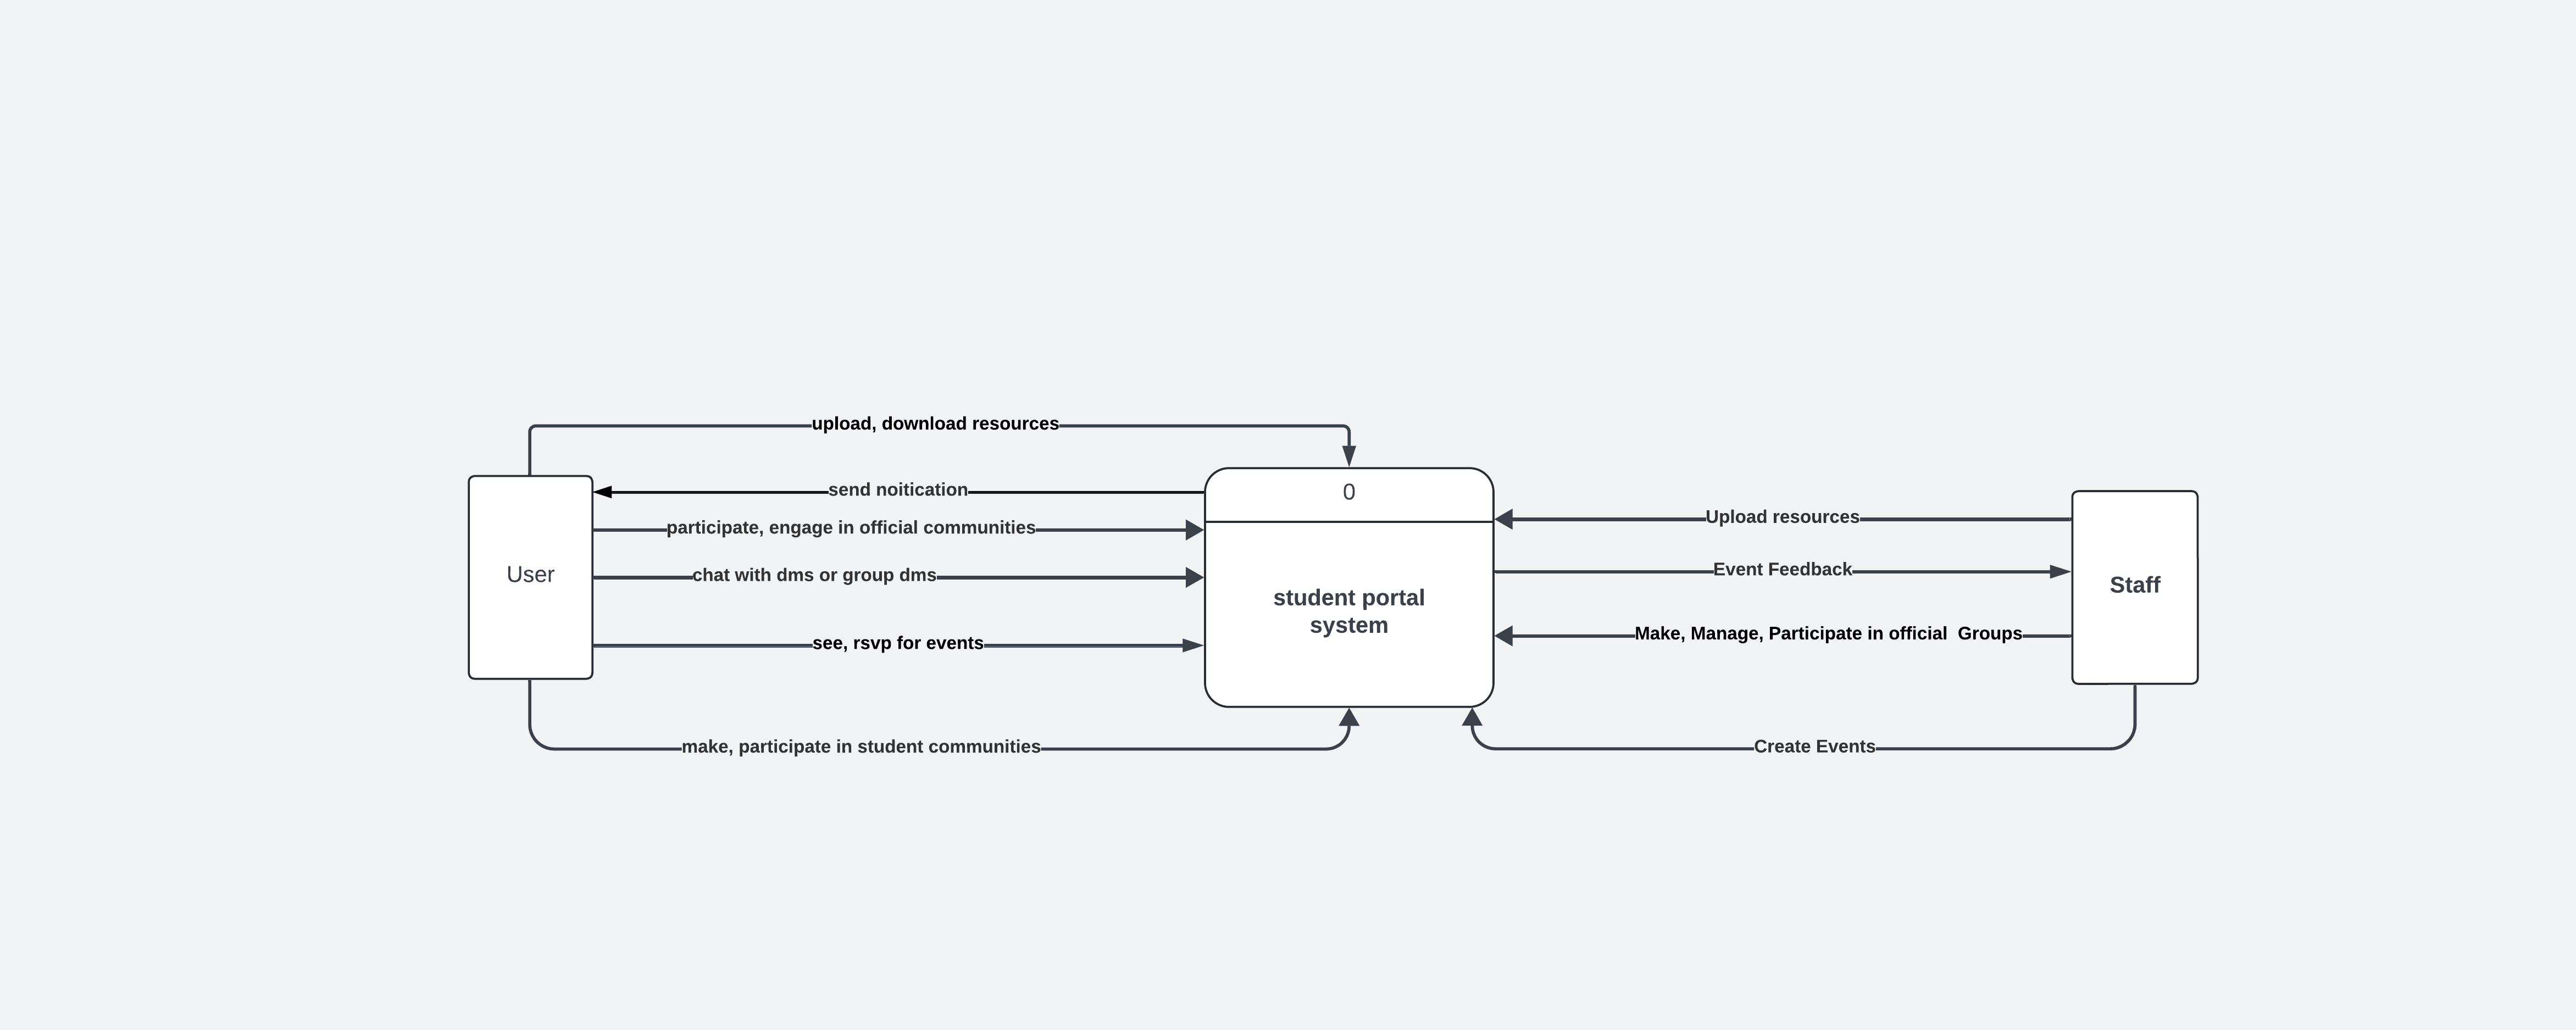
\includegraphics[width=0.8\textwidth]{images/dfd_level0.png}
    \caption{Context diagram showing system boundaries}
    \label{fig:dfd0}
\end{figure}

\subsection{Level 1 DFD}
\begin{figure}[H]
    \centering
    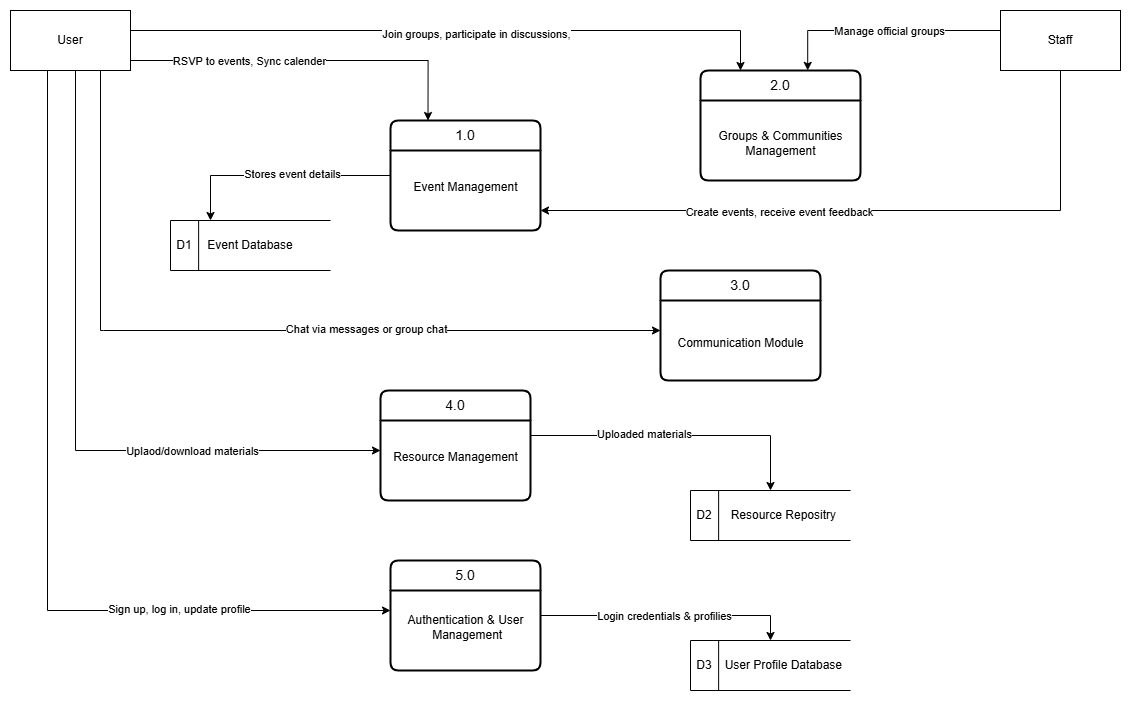
\includegraphics[width=\textwidth]{images/dfd_level1.png}
    \caption{Level 1 DFD showing major subsystems}
    \label{fig:dfd1}
\end{figure}


\vspace{3cm}

\section{Algorithms and Pseudocode}
\label{sec:algorithms}

\subsection{User Authentication}
\begin{algorithm}[H]
\caption{User Authentication Process}\label{alg:auth}
\begin{algorithmic}[1]
\Require email, password
\Ensure Authentication status (success/failure)
\State Validate email and password format
\State Check if user exists in database
\If{user exists}
    \State Verify password hash
    \If{password matches}
        \State Generate JWT token
        \State Store session information
        \State \Return \{token, userData\}
    \Else
        \State \Return "Authentication failed: Invalid credentials"
    \EndIf
\Else
    \State \Return "Authentication failed: User not found"
\EndIf
\end{algorithmic}
\end{algorithm}

\subsection{User Registration}
\begin{algorithm}[H]
\caption{User Registration Process}\label{alg:registration}
\begin{algorithmic}[1]
\Require email, password, userData
\Ensure Registration status
\State Validate email format and password strength
\State Check if email already exists
\If{email is unique}
    \State Generate verification OTP
    \State Send verification email
    \State Store user data with pending status
    \State \Return "Registration initiated"
\Else
    \State \Return "Registration failed: Email already exists"
\EndIf
\end{algorithmic}
\end{algorithm}

\subsection{Email Verification}
\begin{algorithm}[H]
\caption{Email Verification Process}\label{alg:email_verification}
\begin{algorithmic}[1]
\Require email, verificationOTP
\Ensure Verification status
\State Validate OTP format
\State Check OTP expiration
\If{OTP is valid}
    \State Update user email status
    \State Clear verification OTP
    \State \Return "Email verified successfully"
\Else
    \State \Return "Verification failed: Invalid OTP"
\EndIf
\end{algorithmic}
\end{algorithm}

\subsection{Password Management}
\begin{algorithm}[H]
\caption{Password Management Process}\label{alg:password}
\begin{algorithmic}[1]
\Require userId, currentPassword, newPassword
\Ensure Password update status
\State Verify current password
\If{current password is correct}
    \State Validate new password strength
    \State Hash new password
    \State Update password in database
    \State Invalidate existing sessions
    \State \Return "Password updated successfully"
\Else
    \State \Return "Password update failed: Current password incorrect"
\EndIf
\end{algorithmic}
\end{algorithm}

\subsection{User Profile Management}
\begin{algorithm}[H]
\caption{Profile Management Process}\label{alg:profile}
\begin{algorithmic}[1]
\Require userId, profileData
\Ensure Profile update status
\State Validate profile data
\If{profile picture provided}
    \State Upload and process profile picture
\EndIf
\State Update user profile in database
\State Update related user metrics
\State \Return "Profile updated successfully"
\end{algorithmic}
\end{algorithm}

\subsection{Event Management}
\begin{algorithm}[H]
\caption{Event Management Process}\label{alg:event}
\begin{algorithmic}[1]
\Require eventData, userRole
\Ensure Event creation/update status
\State Validate event data
\If{userRole is authorized}
    \State Upload event image if provided
    \State Create/update event in database
    \State Generate calendar integration URLs
    \State \Return \{eventId, calendarUrls\}
\Else
    \State \Return "Unauthorized: Insufficient permissions"
\EndIf
\end{algorithmic}
\end{algorithm}

\subsection{View Events}
\begin{algorithm}[H]
\caption{Event Viewing Process}\label{alg:view_events}
\begin{algorithmic}[1]
\Require userID
\Ensure List of events
\State Retrieve events from the database
\State Filter events based on user preferences (if any)
\State Display events to the user
\end{algorithmic}
\end{algorithm}

\subsection{RSVP Management}
\begin{algorithm}[H]
\caption{RSVP Process}\label{alg:rsvp}
\begin{algorithmic}[1]
\Require userId, eventId, rsvpStatus
\Ensure RSVP status
\State Validate event exists
\If{event exists}
    \State Check if user already has RSVP
    \If{existing RSVP}
        \State Update RSVP status
    \Else
        \State Create new RSVP
    \EndIf
    \State Update event attendee count
    \State \Return "RSVP updated successfully"
\Else
    \State \Return "RSVP failed: Event not found"
\EndIf
\end{algorithmic}
\end{algorithm}

\subsection{Calendar Integration}
\begin{algorithm}[H]
\caption{Calendar Integration Process}\label{alg:calendar}
\begin{algorithmic}[1]
\Require eventId, calendarType
\Ensure Calendar integration URLs
\State Generate event details in iCal format
\State Create calendar-specific URLs
\If{calendarType is Google}
    \State Generate Google Calendar URL
\ElsIf{calendarType is Outlook}
    \State Generate Outlook Calendar URL
\EndIf
\State \Return calendar integration URLs
\end{algorithmic}
\end{algorithm}

\subsection{Sync with Personal Calendars}
\begin{algorithm}[H]
\caption{Calendar Sync Process}\label{alg:calendar_sync}
\begin{algorithmic}[1]
\Require userID, eventID
\Ensure Sync status
\State Retrieve event details using eventID
\If{event exists}
    \State Add event to user's personal calendar (Google Calendar, Outlook)
    \State \Return "Sync successful"
\Else
    \State \Return "Sync failed: Event not found"
\EndIf
\end{algorithmic}
\end{algorithm}

\subsection{Resource Management}
\begin{algorithm}[H]
\caption{Resource Management Process}\label{alg:resource}
\begin{algorithmic}[1]
\Require resourceData, file, userId
\Ensure Resource creation status
\State Validate resource data and file
\State Upload file to storage service
\State Create resource entry in database
\State Initialize metrics (views, downloads, votes)
\State \Return \{resourceId, fileUrl\}
\end{algorithmic}
\end{algorithm}

\subsection{Resource Interaction}
\begin{algorithm}[H]
\caption{Resource Interaction Process}\label{alg:resource_interaction}
\begin{algorithmic}[1]
\Require resourceId, userId, interactionType
\Ensure Interaction status
\State Validate resource exists
\If{interactionType is vote}
    \State Update resource vote count
\ElsIf{interactionType is comment}
    \State Add comment to resource
\ElsIf{interactionType is report}
    \State Create resource report
\EndIf
\State Update resource metrics
\State \Return "Interaction recorded successfully"
\end{algorithmic}
\end{algorithm}

\subsection{Categorized Content Upload}
\begin{algorithm}[H]
\caption{Content Upload Process}\label{alg:content_upload}
\begin{algorithmic}[1]
\Require userID, contentFile, category
\Ensure Content upload status
\State Upload contentFile to the server
\State Store content metadata (userID, category, timestamp) in the database
\State \Return "Content uploaded successfully"
\end{algorithmic}
\end{algorithm}

\subsection{Discussion Participation}
\begin{algorithm}[H]
\caption{Discussion Participation Process}\label{alg:discussion}
\begin{algorithmic}[1]
\Require userID, discussionID, message
\Ensure Participation status
\State Retrieve discussion using discussionID
\If{discussion exists}
    \State Add message to the discussion
    \State Update discussion in the database
    \State \Return "Message posted successfully"
\Else
    \State \Return "Discussion not found"
\EndIf
\end{algorithmic}
\end{algorithm}

\subsection{Direct Messaging}
\begin{algorithm}[H]
\caption{Direct Messaging Process}\label{alg:messaging}
\begin{algorithmic}[1]
\Require senderID, receiverID, message
\Ensure Message send status
\State Store message in the database with senderID, receiverID, and timestamp
\State Notify receiver of the new message
\State \Return "Message sent successfully"
\end{algorithmic}
\end{algorithm}

\subsection{AI-Powered Chatbot}
\begin{algorithm}[H]
\caption{AI Chatbot Response Process}\label{alg:chatbot}
\begin{algorithmic}[1]
\Require userQuery
\Ensure Chatbot response
\State Analyze userQuery using NLP
\State Retrieve most relevant response from FAQ database
\State \Return response to the user
\end{algorithmic}
\end{algorithm}

\subsection{Event Recommendations}
\begin{algorithm}[H]
\caption{Event Recommendation Process}\label{alg:recommendations}
\begin{algorithmic}[1]
\Require userId
\Ensure List of recommended events
\State Retrieve user's past event attendance
\State Get user's interests and preferences
\State Calculate event relevance scores
\State Filter events based on user's schedule
\State Sort events by relevance score
\State \Return top N recommended events
\end{algorithmic}
\end{algorithm}

\subsection{Resource Recommendations}
\begin{algorithm}[H]
\caption{Resource Recommendation Process}\label{alg:resource_recommendations}
\begin{algorithmic}[1]
\Require userId
\Ensure List of recommended resources
\State Get user's download history
\State Analyze user's resource interactions
\State Calculate resource relevance scores
\State Consider resource ratings and popularity
\State \Return top N recommended resources
\end{algorithmic}
\end{algorithm}

\subsection{Recommendation Engine}
\begin{algorithm}[H]
\caption{Content Recommendation Process}\label{alg:recommendation}
\begin{algorithmic}[1]
\Require userID
\Ensure List of recommended content
\State Retrieve user preferences and past interactions
\State Use collaborative filtering algorithm
\State \Return list of recommended content
\end{algorithmic}
\end{algorithm}

\subsection{Announcements Dashboard}
\begin{algorithm}[H]
\caption{Announcements Display Process}\label{alg:announcements}
\begin{algorithmic}[1]
\Require userID
\Ensure List of announcements
\State Retrieve announcements from the database
\State Filter announcements based on user preferences (if any)
\State Display announcements to the user
\end{algorithmic}
\end{algorithm}

\subsection{Mentorship Matching}
\begin{algorithm}[H]
\caption{Mentorship Matching Process}\label{alg:mentorship}
\begin{algorithmic}[1]
\Require userID
\Ensure Matched mentor
\State Retrieve user profile and preferences
\State Calculate compatibility scores with potential mentors
\State \Return best matching mentor
\end{algorithmic}
\end{algorithm}

\subsection{Real-Time Notifications}
\begin{algorithm}[H]
\caption{Notification Process}\label{alg:notifications}
\begin{algorithmic}[1]
\Require userID, notificationMessage
\Ensure Notification status
\State Send notificationMessage to user's device
\State Store notification in the database
\State \Return "Notification sent successfully"
\end{algorithmic}
\end{algorithm} 


\section{Interface Design}
\label{sec:interface_design}
The interfaces were designed with a strong emphasis on usability, accessibility, and consistency. Every screen aligns with the overall system architecture and supports intuitive user workflows.

\subsection*{Design Philosophy}
\begin{itemize}
    \item \textbf{Logical Grouping of Features:} Each section of the interface is contextually structured. For example, in the mobile app, navigation is bottom-tab based, clearly separating Home, Events, Chat, and AI tools. On the web dashboard, admin functionalities like Events, Communities, and Analytics are logically grouped in a sidebar.
    
    \item \textbf{Minimal Cognitive Load:} The design avoids overwhelming users by displaying only relevant information per view. Cards, modals, and tabs are used to reduce visual clutter and enhance clarity.
    
    \item \textbf{Feedback-Oriented Interactions:} All interactive components—buttons, forms, and modals—provide clear feedback (loading indicators, success/error messages), enhancing usability and user trust.
    
    \item \textbf{Responsive and Adaptive Design:} The interfaces automatically adjust layout and font sizes based on screen size, ensuring accessibility on tablets, phones, and desktops.
    
    \item \textbf{Role-Based Views:} The UI dynamically adapts based on user roles (student, admin, instructor). For instance, students only see their events and communities, while admins can manage all users and moderate content.
\end{itemize}


\subsection{Mobile Application Interfaces}
\begin{figure}[h!]
    \centering
    % First row
    \begin{subfigure}{0.3\textwidth}
        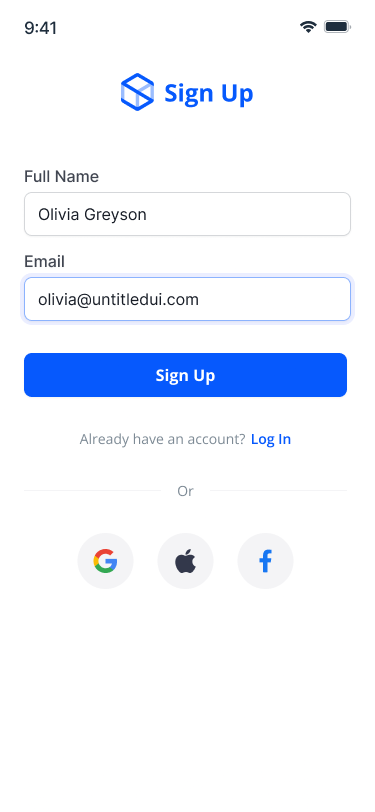
\includegraphics[width=\linewidth]{images/mobile_interface/Sign-up.png}
        \caption{Registration flow}
        \label{fig:signup}
    \end{subfigure}
    \hfill
    \begin{subfigure}{0.3\textwidth}
        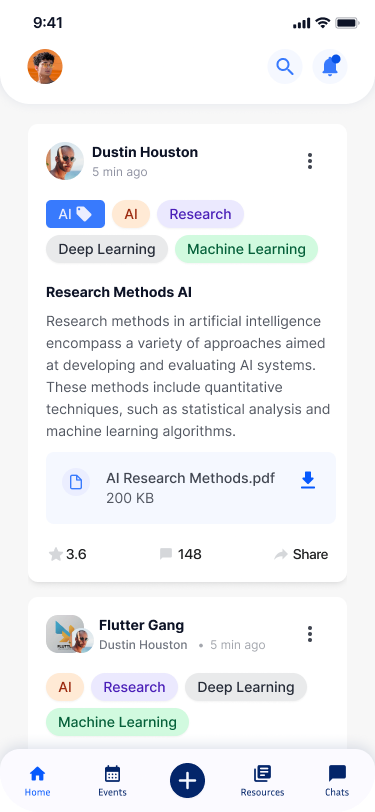
\includegraphics[width=\linewidth]{images/mobile_interface/Home.png}
        \caption{Main activity feed}
        \label{fig:home}
    \end{subfigure}
    \hfill
    \begin{subfigure}{0.3\textwidth}
        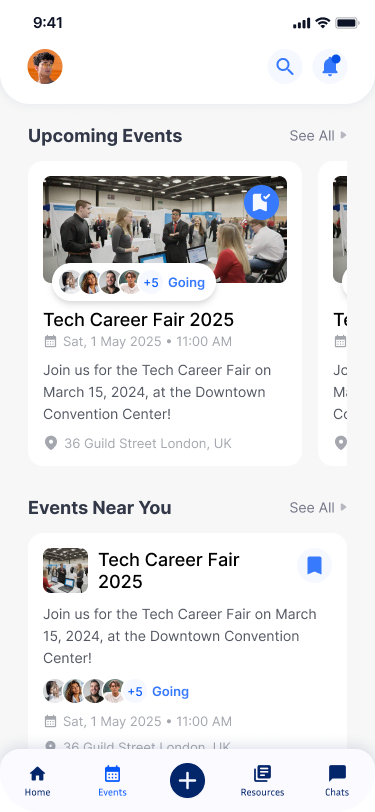
\includegraphics[width=\linewidth]{images/mobile_interface/Events.png}
        \caption{Event discovery}
        \label{fig:events}
    \end{subfigure}
    \vspace{0em} % spacing between rows

    % Second row
    \hfill
    \begin{subfigure}{0.3\textwidth}
        
\includegraphics[width=\linewidth]{images/mobile_interface/Resources.png}
        \caption{Academic resources}
        \label{fig:resources}
    \end{subfigure}
    \hfill
    \begin{subfigure}{0.3\textwidth}
        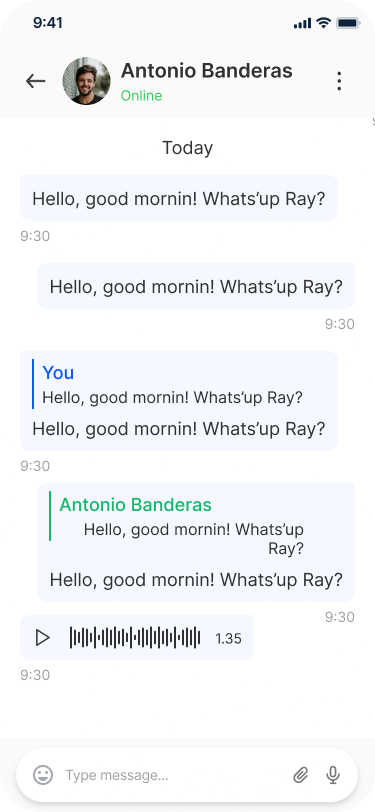
\includegraphics[width=\linewidth]{images/mobile_interface/Chat.png}
        \caption{Messaging interface}
        \label{fig:chat}
    \end{subfigure}
    \hfill
    \begin{subfigure}{0.3\textwidth}
        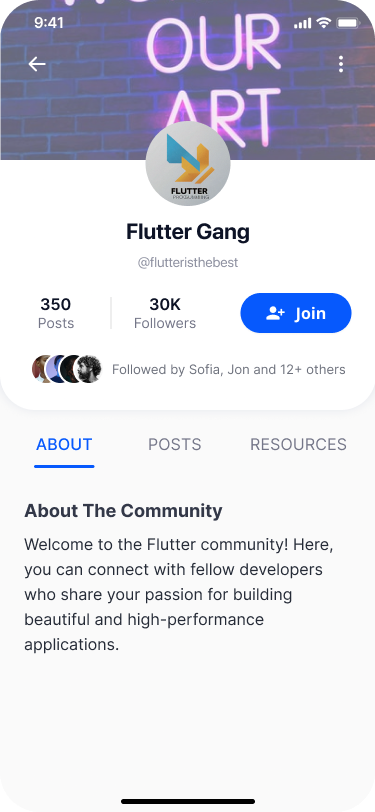
\includegraphics[width=\linewidth]{images/mobile_interface/General-Profile.png}
        \caption{User profile}
        \label{fig:profile}
    \end{subfigure}

    \caption{Mobile Application Interfaces Overview}
    \label{fig:mobile_interfaces}
\end{figure}


\subsection{Admin Dashboard Interfaces}
\begin{figure}[H]
    \centering
    \begin{subfigure}{0.45\textwidth}
        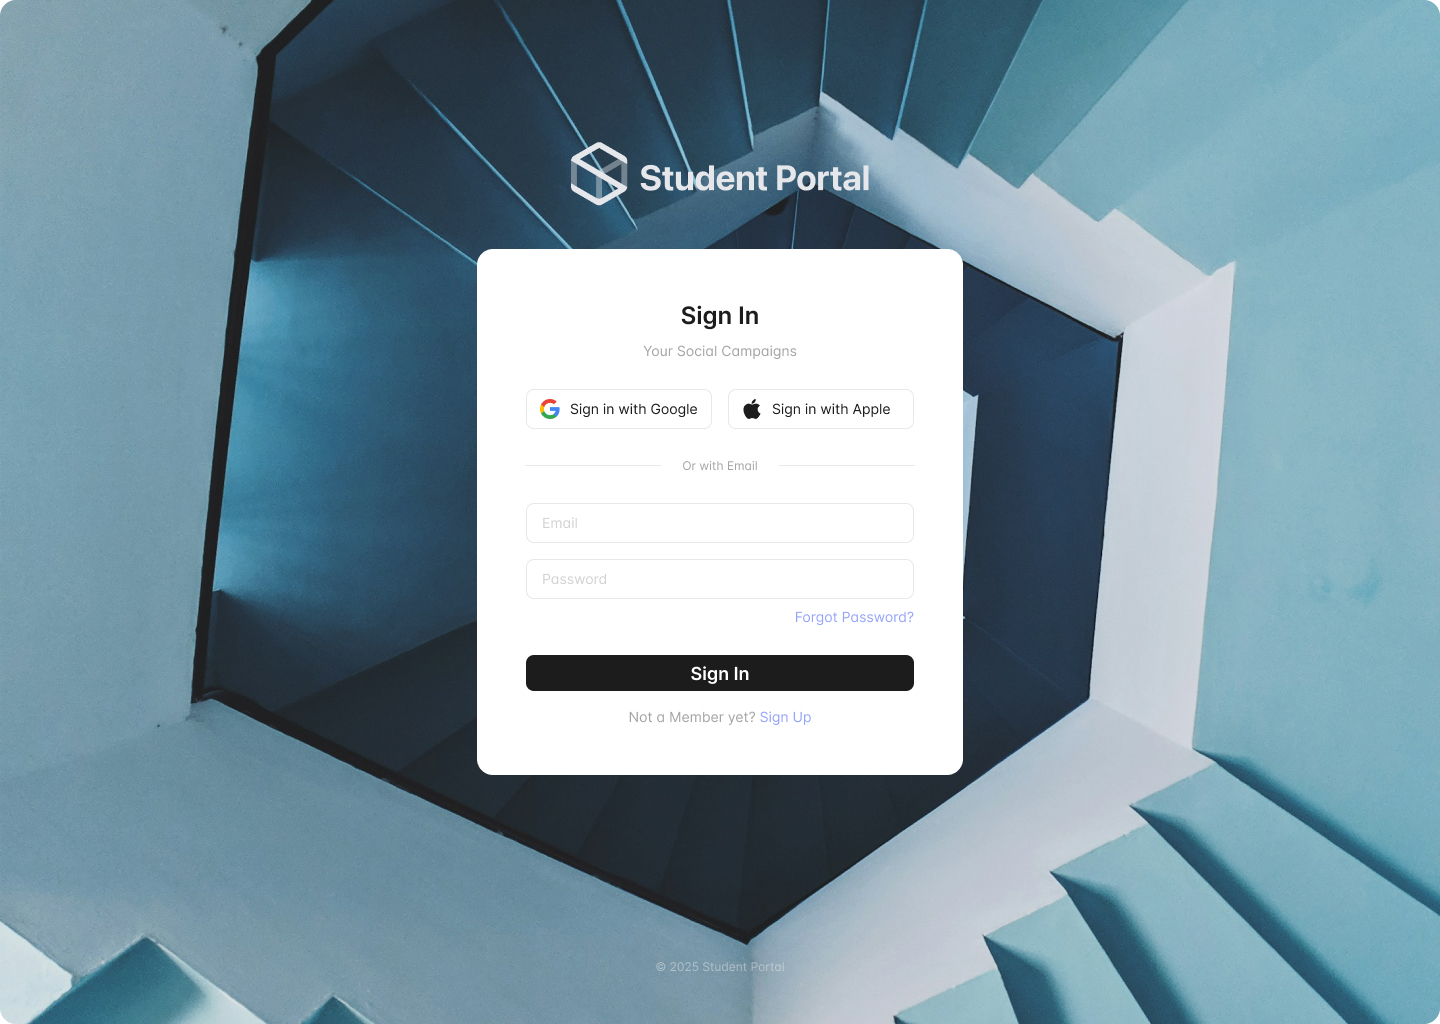
\includegraphics[width=\textwidth]{images/web_interface/Authentication-Sign_In.jpg}
        \caption{Admin login screen}
        \label{fig:admin_login}
    \end{subfigure}
    \begin{subfigure}{0.45\textwidth}
        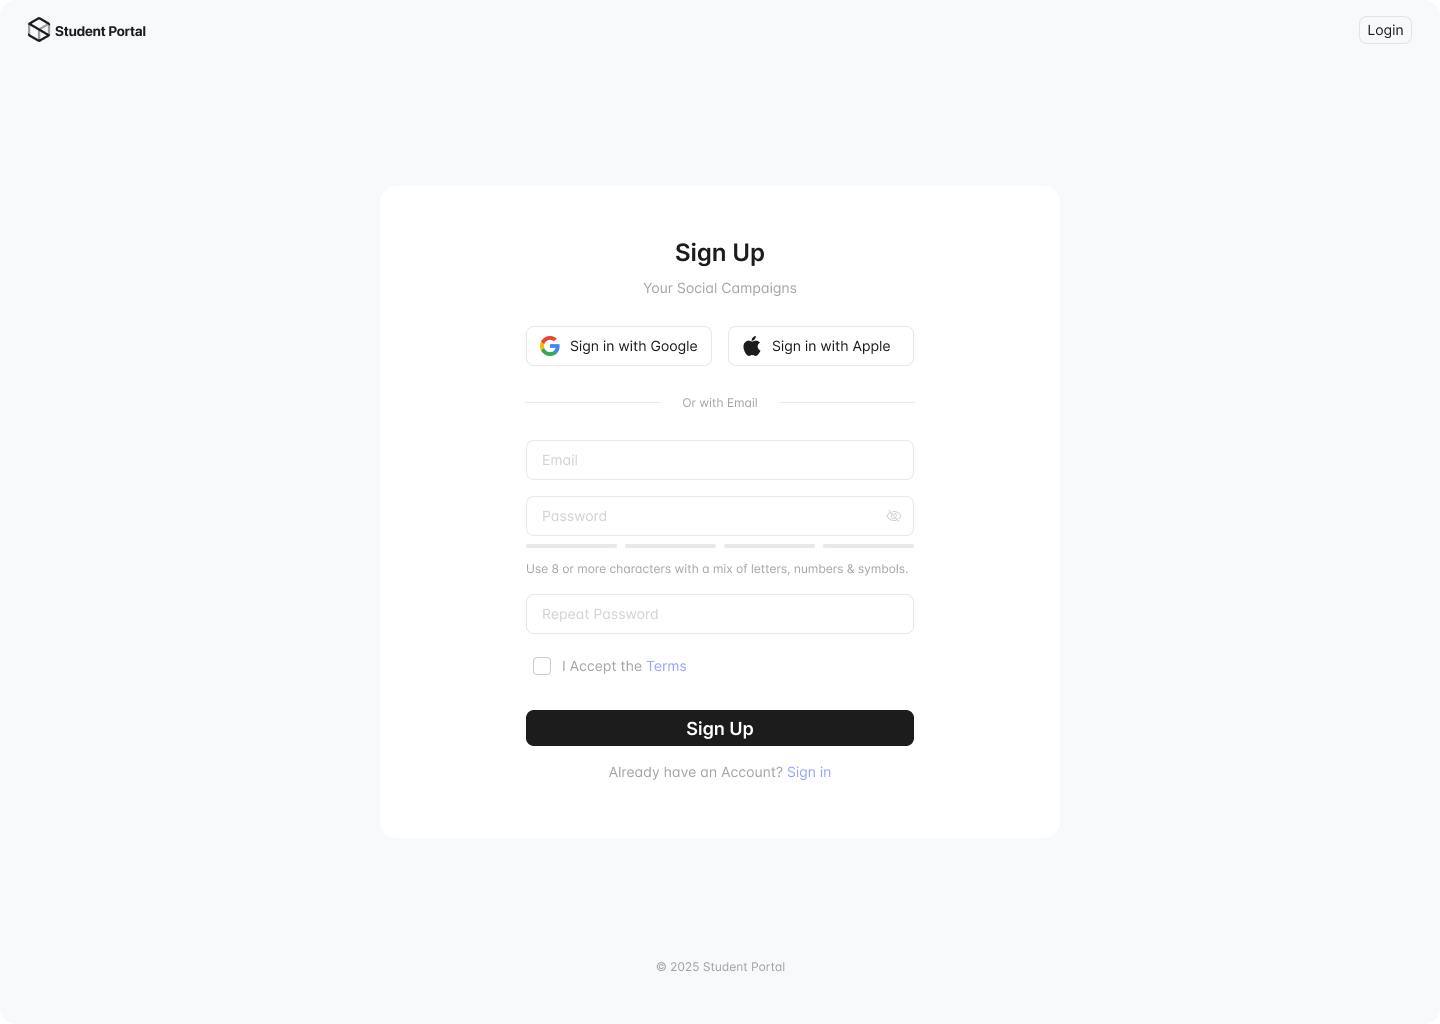
\includegraphics[width=\textwidth]{images/web_interface/Authentication-Sign_Up.jpg}
        \caption{Admin account creation}
        \label{fig:admin_signup}
    \end{subfigure}
    \caption{Admin portal authentication flows}
    \label{fig:admin_auth}
\end{figure}

\begin{figure}[H]
    \centering
    \begin{subfigure}{0.45\textwidth}
        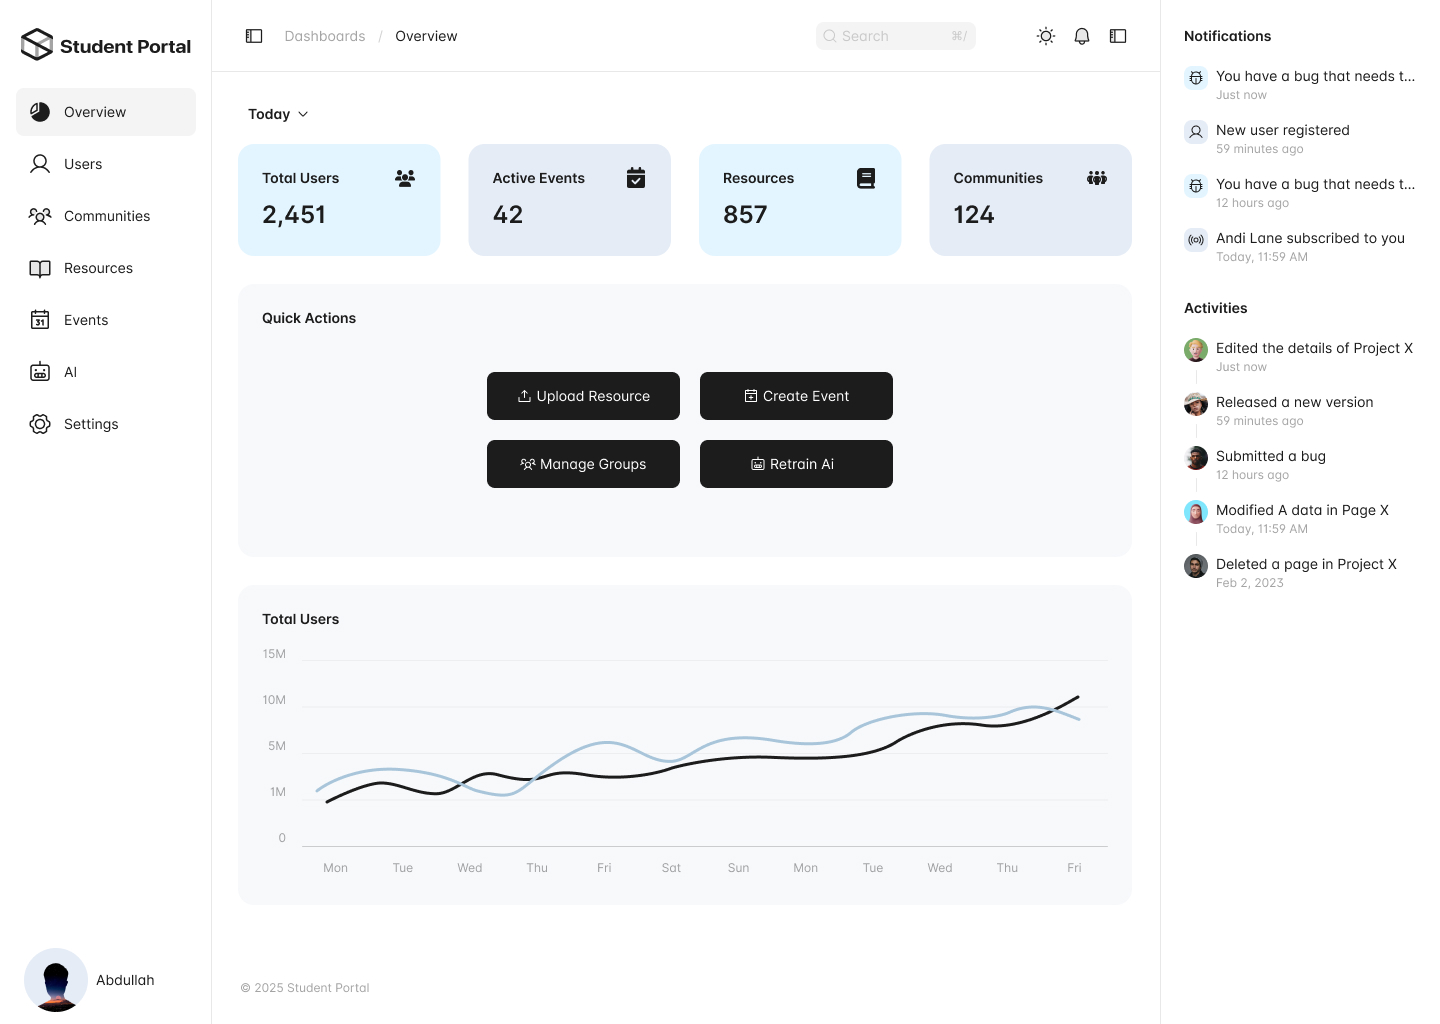
\includegraphics[width=\textwidth]{images/web_interface/Overview.jpg}
        \caption{Dashboard overview}
        \label{fig:overview}
    \end{subfigure}
    \begin{subfigure}{0.45\textwidth}
        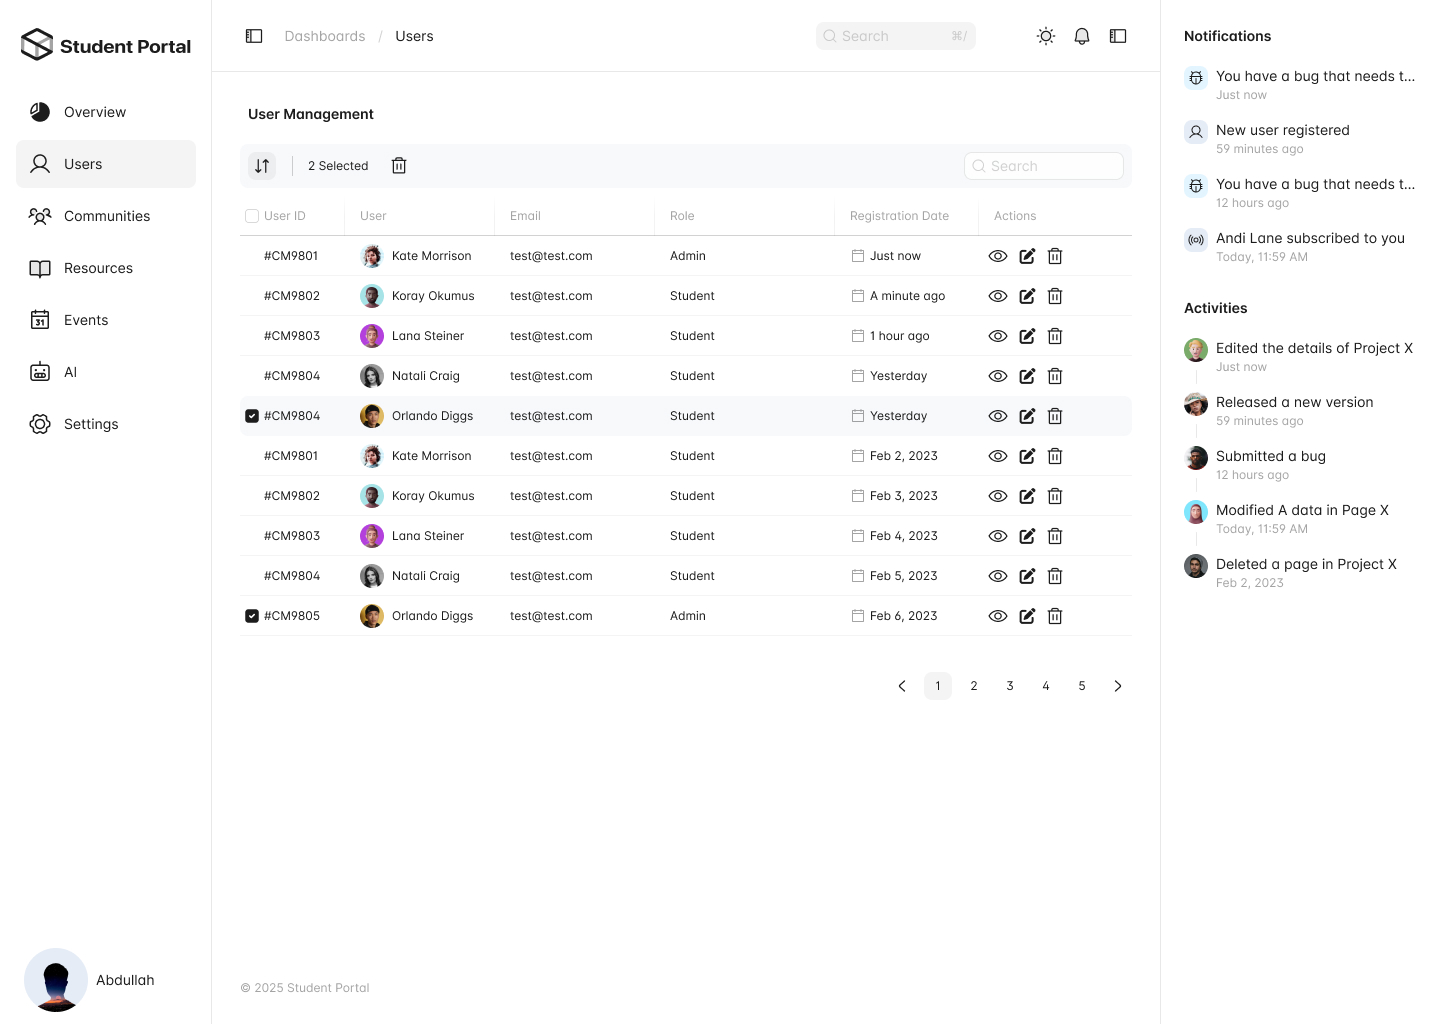
\includegraphics[width=\textwidth]{images/web_interface/User-Management.jpg}
        \caption{User management console}
        \label{fig:user_mgmt}
    \end{subfigure}
    \caption{Admin dashboard main views}
    \label{fig:admin_main}
\end{figure}

\begin{figure}[H]
    \centering
    \begin{subfigure}{0.45\textwidth}
        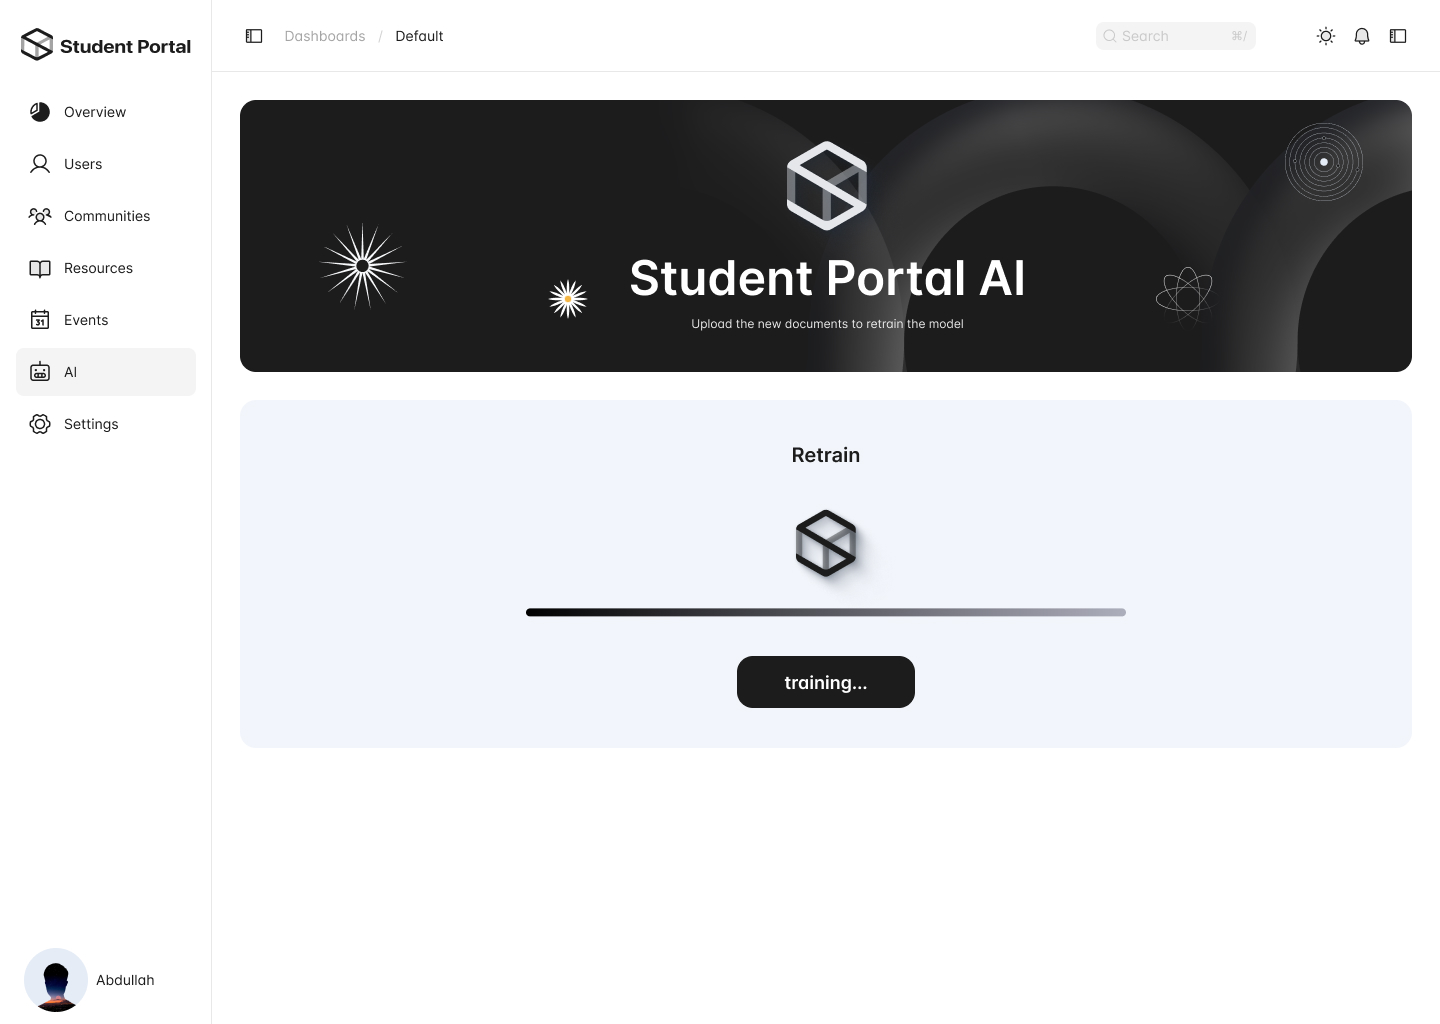
\includegraphics[width=\textwidth]{images/web_interface/AI-training.jpg}
        \caption{AI model training interface}
        \label{fig:ai_training}
    \end{subfigure}
    \begin{subfigure}{0.45\textwidth}
        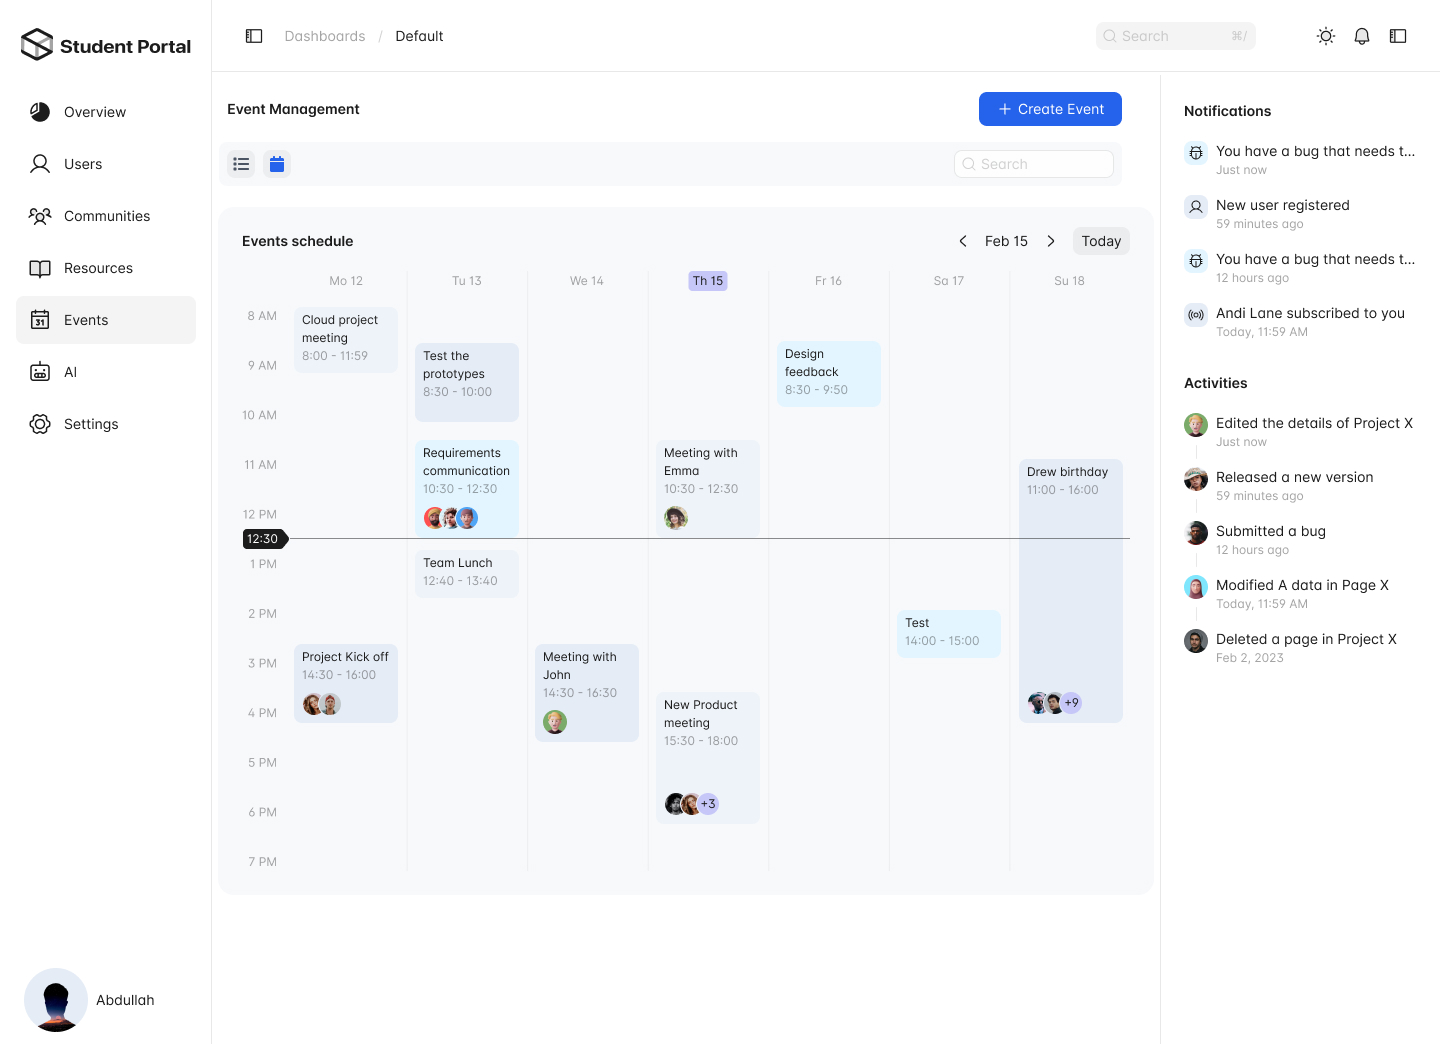
\includegraphics[width=\textwidth]{images/web_interface/Event-Management-cal.jpg}
        \caption{Event moderation panel}
        \label{fig:event_mgmt}
    \end{subfigure}
    \caption{Specialized admin tools}
    \label{fig:admin_tools}
\end{figure}

\chapter{Implementation Aspects}
\label{chap:implementation}

\section{Overall System Architecture}
\label{sec:system_architecture}

\subsection{Layered Architecture}

\textbf{Client Layer}
\begin{itemize}
    \item \textbf{Web App (Nextjs + React)}: Dashboard, resource upload, mentorship matching
    \item \textbf{Mobile App (Flutter)}: Notifications, calendar sync, community discussions
\end{itemize}

\textbf{Backend Layer}
\begin{itemize}
    \item \textbf{Auth Service}: JWT token generation, MFA
    \item \textbf{Event Service}: Manages event creation, RSVPs, and Google Calendar sync
    \item \textbf{Community Service}: Handles group creation, discussions, and mentorship tools
\end{itemize}

\textbf{AI Layer}
\begin{itemize}
    \item \textbf{Chatbot Service}: Flask API + Dialogflow (answers university queries)
    \item \textbf{Recommendation Service}: TensorFlow model for personalized suggestions
\end{itemize}

\textbf{Storage Layer}
\begin{itemize}
    \item \textbf{MongoDB Atlas}: User profiles, events, and community data
    \item \textbf{Elasticsearch}: Resource search and discovery
\end{itemize}

\textbf{Security Layer}
\begin{itemize}
    \item \textbf{API Gateway}: Kong/Express Gateway (rate limiting, JWT validation)
    \item \textbf{Encryption}: AES-256 (data at rest), TLS 1.3 (data in transit)
\end{itemize}

\textbf{Integration Layer}
\begin{itemize}
    \item \textbf{Third-Party APIs}: Google Calendar, Firebase, Twilio
\end{itemize}

\subsection{Data Flow}
\begin{enumerate}
    \item Users interact via React/Flutter clients
    \item Requests pass through API Gateway for security checks
    \item Node.js backend processes CRUD operations
    \item AI services provide real-time responses and recommendations
    \item Real-time notifications (Socket.io/FCM) and calendar sync
\end{enumerate}

\subsection{Architecture Justification}
\begin{itemize}
    \item \textbf{Modularity}: Separates concerns for scalability
    \item \textbf{Agile Alignment}: Supports iterative development sprints
    \item \textbf{Compliance}: Meets security NFRs (encryption, audits) and usability goals
\end{itemize}

\section{Tools and Technologies}
\label{sec:tools_tech}

\textbf{Design}
\begin{itemize}
    \item Figma: Industry-standard UI/UX design tool used for creating wireframes, prototypes, and high-fidelity designs with collaborative features
    \item Lucidchart: Cloud-based diagramming software for creating system architecture diagrams, flowcharts, and UML diagrams with real-time collaboration
\end{itemize}

\textbf{Backend}
\begin{itemize}
    \item Framework: Express.js
    \item Database: MongoDB
    \item Real-Time: Socket.io
    \item Authentication: JWT
    \item Testing: Postman
    \item CI/CD: GitHub Actions
\end{itemize}

\textbf{Frontend}
\begin{itemize}
    \item State Management: React Hook Form, Props drilling (max 2 levels)
    \item UI Libraries: Shadcn ui, styled-components
    \item Routing: Next js app router (folder / file based routing)
\end{itemize}

\textbf{Mobile}
\begin{itemize}
    \item Framework: Flutter
    \item State Management: Provider
    \item Notifications: Firebase Cloud Messaging
    \item Local Storage: Hive
\end{itemize}


\textbf{AI Components}
\begin{itemize}
    \item Chatbot: Python with PyTorch and FastAPI
    \item Recommendation System: PyTorch with FastAPI
\end{itemize}


\textbf{Security}
\begin{itemize}
    \item Encryption: TLS/SSL, bcrypt
    \item Access Control: Role-Based Access Control (RBAC)
    \item Vulnerability Scanning: OWASP ZAP
\end{itemize}

\textbf{Infrastructure}
\begin{itemize}
    \item Hosting: AWS EC2, Vercel
    \item Containerization: Docker
    \item Monitoring: Prometheus, Grafana
\end{itemize}

\subsection{Integration Highlights}
\begin{itemize}
    \item \textbf{Calendar Sync}: Google Calendar API integration
    \item \textbf{File Storage}: Firebase Storage/Amazon S3 for academic resources
    \item \textbf{Search}: Elasticsearch implementation
    \item \textbf{Project Management}: Trello for sprint planning
    \item \textbf{Collaboration}: Slack/Discord for team coordination
\end{itemize}
\lstset{style=mystyle}

\section{Implementation}
\label{sec:implementation}

\subsection{Introduction}
\label{subsec:introduction}

This chapter provides a detailed walkthrough of the implementation process for the Student Portal project. The platform is structured into four major components: the backend server, web application, mobile application, and AI/ML services. Each component is managed collaboratively via our GitHub organization using issue tracking, pull requests, and continuous integration.

\subsubsection{System Architecture Highlights}

\begin{itemize}
    \item \textbf{Backend:} Node.js with TypeScript, following a repository-service-controller pattern. Mongoose handles the database layer, and the codebase is organized into modular folders.
    
    \item \textbf{Web Application:} Built with Next.js and styled with Tailwind CSS. Uses TanStack Query for state management and React Hook Form for form handling.
    
    \item \textbf{Mobile Application:} Built in Flutter with a clean architecture using the BLoC pattern. Each feature has its own folder containing BLoC, use cases, UI, and data layer.
    
    \item \textbf{AI/ML Services:} Python-based services using PyTorch, FAISS, and Flask. Modular design separates chatbot, recommendation, and inference code.
\end{itemize}

\subsection{GitHub Organization and Workflow}
\label{subsec:github_workflow}

Our project is managed through a dedicated GitHub organization that serves as the central hub for collaboration, code management, and project tracking. The organization structure and workflow are designed to facilitate efficient team collaboration and maintain high code quality standards.

\subsubsection{Organization Structure}
\label{subsubsec:org_structure}

The GitHub organization is organized into several key repositories:

\begin{itemize}
    \item \textbf{student-portal-server}: Backend server implementation
    \item \textbf{student-portal-web}: Next.js web application
    \item \textbf{student-portal-app}: Flutter mobile application
    \item \textbf{student-portal-ai}: AI/ML models and services
    \item \textbf{student-portal-docs}: Project documentation and guides
\end{itemize}

\begin{figure}[h]
    \centering
    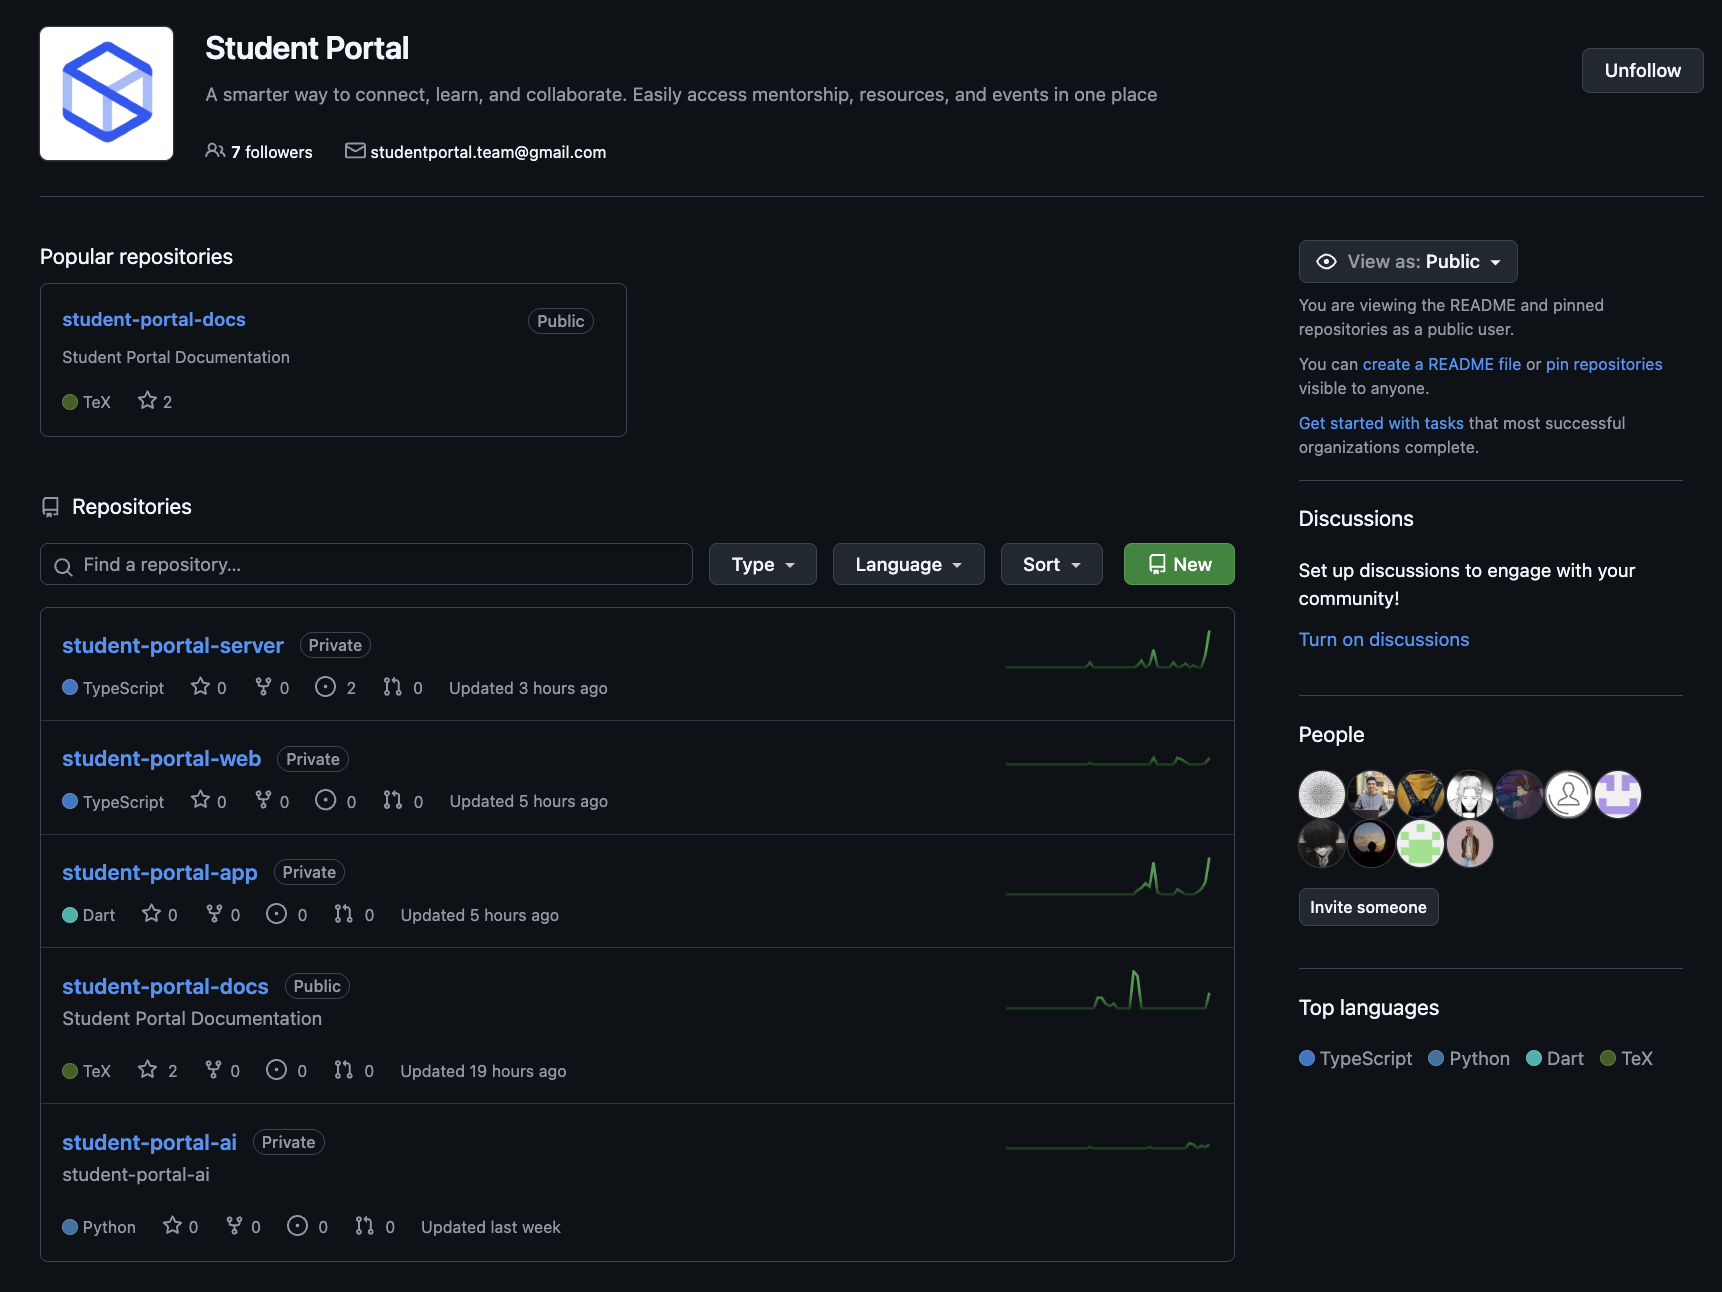
\includegraphics[width=0.8\textwidth]{images/github-org-overview}
    \caption{GitHub Organization Overview}
    \label{fig:github_org}
\end{figure}

\subsubsection{Development Workflow}
\label{subsubsec:dev_workflow}

Our development process is built on efficient collaboration and high-quality standards. We maintain a structured Git workflow with clear branching strategies and automated pipelines. Discord meetings keep the team aligned, while our comprehensive documentation ensures smooth knowledge sharing. The combination of agile practices and automated testing allows us to deliver features while maintaining code quality.

\subsection{Frontend Screens}
\label{subsec:frontend_screens}

\subsubsection{Web Application Screens}
\label{subsubsec:web_screens}

\begin{itemize}
    \item \textbf{Student Dashboard:} A modern, responsive dashboard with activity feed, quick access to events, performance metrics, and personalized recommendations.
    
    \item \textbf{Event Management Portal:} Interactive calendar interface with event creation wizard, attendee management, and automated notifications.
    
    \item \textbf{Community Hub:} Member directory with role management, discussion forums, and resource sharing capabilities.
    
    \item \textbf{AI Learning Assistant:} Real-time chat interface with progress tracking and personalized study recommendations.
\end{itemize}

% Web Application Screenshots
\begin{figure}[h]
    \centering
    \begin{subfigure}[b]{0.45\textwidth}
        \centering
        % \includegraphics[width=\textwidth]{images/web-dashboard.png}
        \caption{Student Dashboard}
        \label{fig:web-dashboard}
    \end{subfigure}
    \hfill
    \begin{subfigure}[b]{0.45\textwidth}
        \centering
        % \includegraphics[width=\textwidth]{images/web-events.png}
        \caption{Event Management}
        \label{fig:web-events}
    \end{subfigure}
    \vskip\baselineskip
    \begin{subfigure}[b]{0.45\textwidth}
        \centering
        % \includegraphics[width=\textwidth]{images/web-community.png}
        \caption{Community Hub}
        \label{fig:web-community}
    \end{subfigure}
    \hfill
    \begin{subfigure}[b]{0.45\textwidth}
        \centering
        % \includegraphics[width=\textwidth]{images/web-ai-assistant.png}
        \caption{AI Learning Assistant}
        \label{fig:web-ai}
    \end{subfigure}
    \caption{Web Application Screens}
    \label{fig:web_screens}
\end{figure}

\subsubsection{Mobile Application Screens}
\label{subsubsec:mobile_screens}

\begin{itemize}
    \item \textbf{Home Feed:} Personalized mobile dashboard with swipeable activity cards and quick actions.
    
    \item \textbf{Event Explorer:} Location-aware event discovery with one-tap registration and offline support.
    
    \item \textbf{Smart Search:} Voice-enabled search with real-time suggestions and category filtering.
    
    \item \textbf{Messaging Center:} Real-time messaging with file sharing and media preview capabilities.
\end{itemize}

% Mobile Application Screenshots
\begin{figure}[H]
    \centering
    \begin{subfigure}[b]{0.22\textwidth}
        \centering
        % 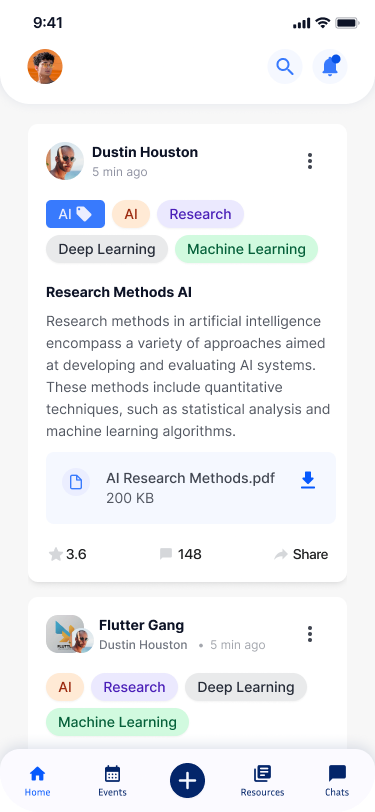
\includegraphics[width=\textwidth,height=0.3\textheight,keepaspectratio]{images/mobile-home.png}
        \caption{Home Feed}
        \label{fig:mobile-home}
    \end{subfigure}
    \hfill
    \begin{subfigure}[b]{0.22\textwidth}
        \centering
        % 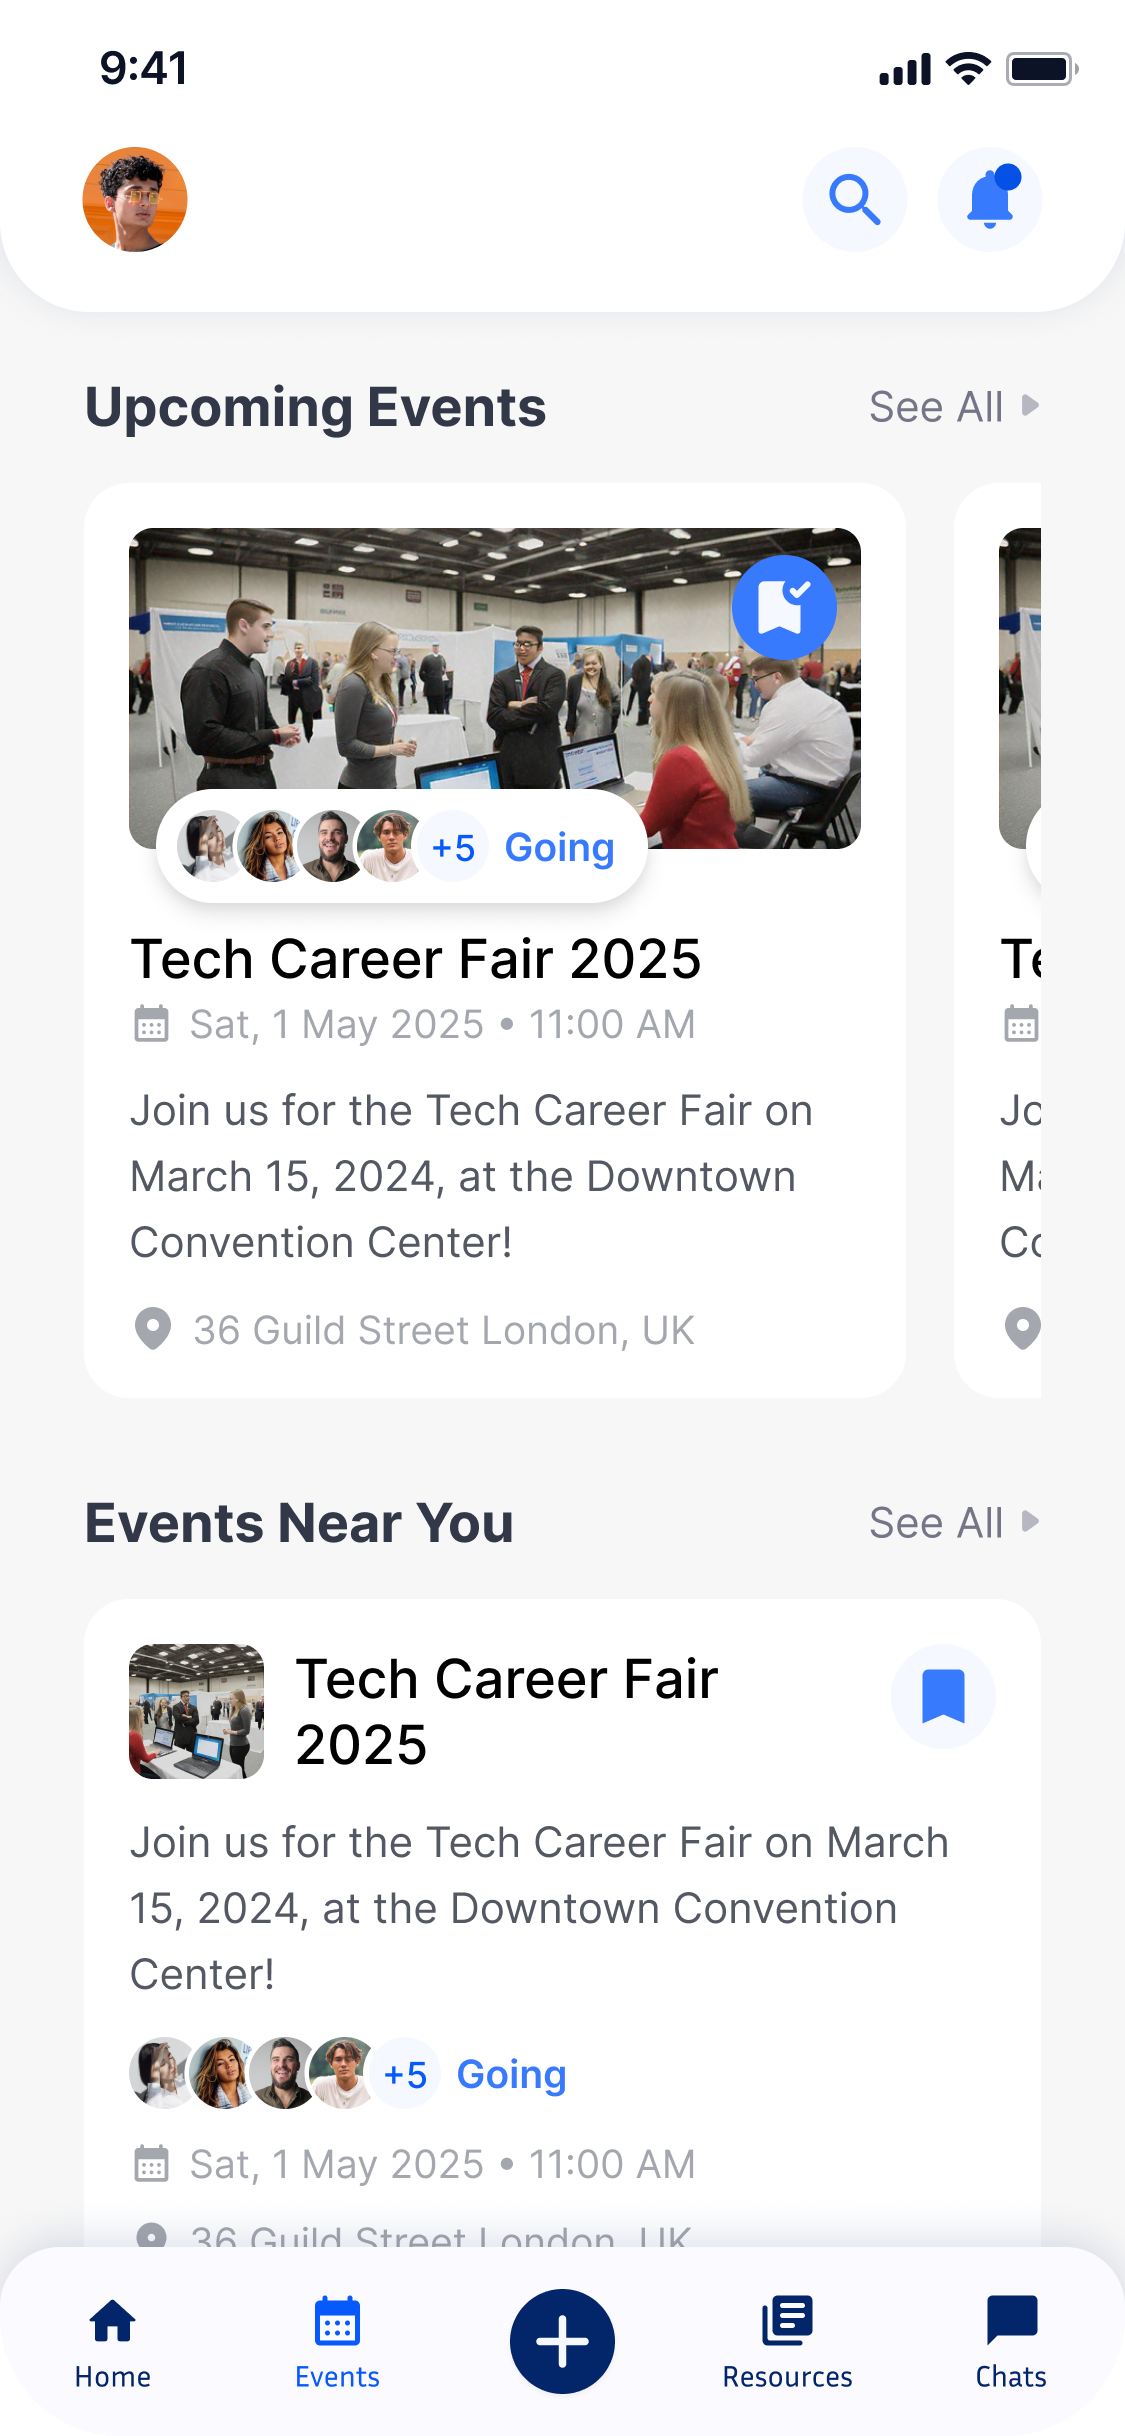
\includegraphics[width=\textwidth,height=0.3\textheight,keepaspectratio]{images/mobile-events.png}
        \caption{Event Explorer}
        \label{fig:mobile-events}
    \end{subfigure}
    \hfill
    \begin{subfigure}[b]{0.22\textwidth}
        \centering
        % \includegraphics[width=\textwidth,height=0.3\textheight,keepaspectratio]{images/mobile-search.png}
        \caption{Smart Search}
        \label{fig:mobile-search}
    \end{subfigure}
    \hfill
    \begin{subfigure}[b]{0.22\textwidth}
        \centering
        % \includegraphics[width=\textwidth,height=0.3\textheight,keepaspectratio]{images/mobile-messaging.png}
        \caption{Messaging Center}
        \label{fig:mobile-messaging}
    \end{subfigure}
    \caption{Mobile Application Screens}
    \label{fig:mobile_screens}
\end{figure}

Each screen is designed with a focus on user experience, accessibility, and performance. The interfaces follow material design principles and maintain consistency across platforms while adapting to the unique capabilities of each device type.

\subsection{Project File Structure Overview}
\label{subsec:file_structure}

Below is the structured layout of each major component of the Student Portal project, showing the first two levels of the directory structure:

\subsubsection{Backend (Node.js + TypeScript)}

\begin{lstlisting}[language=bash, caption={Backend Directory Structure (tree -L 2)}]
backend/
├── __tests__/
├── docs/
├── src/
│   ├── config/          # Environment and app configuration
│   ├── controllers/     # Request handlers and route logic
│   ├── interfaces/      # TypeScript type definitions
│   ├── libs/           # Third-party library integrations
│   ├── middleware/     # Express middleware functions
│   ├── models/         # Mongoose schema definitions
│   ├── repositories/   # Data access layer
│   ├── routes/         # API route definitions
│   ├── services/       # Business logic layer
│   ├── types/          # Custom type definitions
│   ├── utils/          # Helper functions
│   └── validators/     # Input validation schemas
├── package.json        # Project dependencies
├── tsconfig.json      # TypeScript configuration
└── server.ts          # Application entry point
\end{lstlisting}

\begin{tcolorbox}[title=Backend Architecture]
The backend follows the \textbf{repository-service-controller} pattern to ensure separation of concerns and maintainability. Each layer has a specific responsibility:
\begin{itemize}
    \item \textbf{Controllers}: Handle HTTP requests and responses
    \item \textbf{Services}: Implement business logic
    \item \textbf{Repositories}: Manage data access and persistence
\end{itemize}
\end{tcolorbox}

\subsubsection{Web Application (Next.js + Tailwind CSS)}

\begin{lstlisting}[language=bash, caption={Web Application Directory Structure (tree -L 2)}]
web/
├── app/                # Next.js 13+ app directory
├── components/         # React components
│   ├── buttons/       # Reusable button components
│   ├── forms/         # Form components and validation
│   ├── navigation/    # Navigation and routing components
│   └── ui/            # UI components and layouts
├── lib/               # Utility functions and hooks
│   ├── hooks/         # Custom React hooks
│   └── utils.ts       # Helper functions
├── public/            # Static assets
│   ├── icons/         # SVG and icon assets
│   ├── logos/         # Brand and logo files
│   └── pics/          # Image assets
├── middleware.ts      # Next.js middleware
├── routes.ts          # Route definitions
└── next.config.ts     # Next.js configuration
\end{lstlisting}

\begin{tcolorbox}[title=Web Architecture]
The web application uses \textbf{modular foldering}, custom hooks, and utility-first styling with Tailwind. Key features include:
\begin{itemize}
    \item \textbf{TanStack Query}: For server state management
    \item \textbf{React Hook Form}: For form handling and validation
    \item \textbf{Next.js App Router}: For file-based routing
    \item \textbf{Tailwind CSS}: For utility-first styling
\end{itemize}
\end{tcolorbox}

\subsubsection{Mobile Application (Flutter + BLoC Pattern)}

\begin{lstlisting}[language=bash, caption={Mobile Application Directory Structure (tree -L 2)}]
app/
├── assets/          # Static assets
│   ├── fonts/      # Custom fonts
│   ├── icons/      # App icons
│   └── images/     # Image assets
├── lib/            # Dart source code
│   ├── core/       # Core functionality
│   ├── features/   # Feature modules
│   ├── main.dart   # App entry point
│   └── widgets/    # Reusable widgets
├── ios/            # iOS platform code
├── android/        # Android platform code
├── pubspec.yaml    # Dependencies
└── test/           # Test files
\end{lstlisting}

\begin{tcolorbox}[title=Mobile Architecture]
The mobile app follows \textbf{clean architecture} and the \textbf{BLoC pattern}, where each feature encapsulates its logic in \texttt{lib/features/<feature\_name>}. Key aspects:
\begin{itemize}
    \item \textbf{BLoC Pattern}: For state management
    \item \textbf{Feature-first}: Each feature is self-contained
    \item \textbf{Platform-specific}: Separate iOS and Android code
    \item \textbf{Widget-based}: Reusable UI components
\end{itemize}
\end{tcolorbox}

\subsubsection{AI/ML Services (Python + PyTorch + Flask)}

\begin{lstlisting}[language=bash, caption={AI/ML Services Directory Structure (tree -L 2)}]
ai/
├── chatbot/           # Chatbot service
│   ├── models/        # ML model definitions
│   ├── api/           # Flask API endpoints
│   ├── inference/     # Model inference code
│   └── train_model.py # Model training script
├── recommendation/    # Recommendation service
│   ├── models/        # ML model definitions
│   ├── api/           # Flask API endpoints
│   ├── model_trainer.py # Model training script
│   └── demo.py        # Demo and testing
├── requirements.txt   # Python dependencies
└── README.md         # Documentation
\end{lstlisting}

\begin{tcolorbox}[title=AI/ML Architecture]
The AI system is split into \textbf{chatbot} and \textbf{recommendation} modules, each containing:
\begin{itemize}
    \item \textbf{Model Training}: PyTorch-based model training
    \item \textbf{API Endpoints}: Flask-based REST APIs
    \item \textbf{Inference}: Real-time model inference
    \item \textbf{Documentation}: Usage and deployment guides
\end{itemize}
\end{tcolorbox}

\subsection{Code Implementation Examples}
\label{subsec:code_examples}

\subsubsection{Backend Implementation}
\label{subsubsec:backend_examples}

\paragraph{User Repository}
The user repository demonstrates clean separation of data access logic:

\begin{lstlisting}[language=TypeScript, caption={User Repository Implementation}]
/**
 * User Repository - Handles all database operations for users
 */
export class UserRepository {
    /**
     * Find user by email with type safety
     * @param email - User's email address
     * @returns User document or null if not found
     */
    static async findByEmail(email: string): Promise<IUserDocument | null> {
        return User.findOne({ email });
    }

    /**
     * Create new user with validation
     * @param userData - User data to create
     * @returns Created user document
     */
    static async create(userData: Partial<IUserDocument>): Promise<IUserDocument> {
        const user = await User.create(userData);
        return user;
    }

    /**
     * Update user profile with error handling
     * @param userId - User's ID
     * @param updateData - Data to update
     * @returns Updated user document
     */
    static async updateProfile(
        userId: Types.ObjectId,
        updateData: Partial<IUserDocument>
    ): Promise<IUserDocument | null> {
        const user = await User.findByIdAndUpdate(
            userId,
            { $set: updateData },
            { new: true }
        ).select('-password');
        
        if (!user) {
            throw new AppError(
                'User not found',
                HttpStatus.NOT_FOUND,
                ErrorCodes.NOT_FOUND
            );
        }
        
        return user;
    }

    /**
     * Get user with populated fields
     */
    static async getUserWithDetails(userId: Types.ObjectId): Promise<IUserDocument | null> {
        return User.findById(userId)
            .populate('communities', 'name')
            .populate('events', 'title dateTime')
            .select('-password');
    }
}
\end{lstlisting}

\paragraph{Authentication Service}
The authentication service demonstrates business logic implementation:

\begin{lstlisting}[language=TypeScript, caption={Authentication Service Implementation}]
/**
 * Authentication Service - Handles user authentication and authorization
 */
export class AuthService {
    /**
     * User registration with email verification
     * @param userData - User registration data
     * @returns Created user and success message
     */
    static async signup(userData: any) {
        // Check for existing user
        const existingUser = await UserRepository.findByEmail(userData.email);
        if (existingUser) {
            throw new AppError(
                'Email already registered',
                HttpStatus.CONFLICT,
                ErrorCodes.DUPLICATE_ENTRY
            );
        }

        // Create user with hashed password
        const hashedPassword = await hashPassword(userData.password);
        const user = await UserRepository.create({
            ...userData,
            password: hashedPassword,
            status: 'pending'
        });

        // Send verification email
        await sendEmail({
            to: user.email,
            subject: 'Verify your email',
            template: 'verification',
            data: { token: verificationToken }
        });

        return { user, message: 'Registration successful' };
    }

    /**
     * User login with credential validation
     * @param email - User's email
     * @param password - User's password
     * @returns User data and JWT token
     */
    static async login(email: string, password: string) {
        const user = await UserRepository.findByEmail(email);
        if (!user || !(await comparePassword(password, user.password))) {
            throw new AppError(
                'Invalid credentials',
                HttpStatus.UNAUTHORIZED,
                ErrorCodes.AUTHENTICATION_ERROR
            );
        }

        const token = generateToken(user._id);
        return { user, token };
    }
}
\end{lstlisting}

\paragraph{Notification Service}
The notification service demonstrates multi-channel notification delivery:

\begin{lstlisting}[language=TypeScript, caption={Notification Service Implementation}]
/**
 * Notification Service - Handles multi-channel notification delivery
 */
export class NotificationService {
    /**
     * Send notification through multiple channels
     * @param params - Notification parameters
     * @returns Created notification
     */
    static async sendNotification(params: {
        userId: Types.ObjectId;
        type: 'EVENT' | 'MESSAGE' | 'SYSTEM';
        title: string;
        message: string;
        data?: Record<string, any>;
        channels?: ('email' | 'push' | 'in-app')[];
    }) {
        const { userId, type, title, message, data, channels = ['in-app'] } = params;

        // Create notification record
        const notification = await NotificationRepository.create({
            userId,
            type,
            title,
            message,
            data
        });

        // Get user preferences
        const user = await User.findById(userId).select('email notificationPreferences');
        if (!user) {
            throw new AppError('User not found', HttpStatus.NOT_FOUND);
        }

        // Send through preferred channels
        if (channels.includes('email') && user.notificationPreferences?.email) {
            await sendEmail({
                to: user.email,
                subject: title,
                template: 'notification',
                data: { title, message, ...data }
            });
        }

        return notification;
    }
}
\end{lstlisting}

\subsubsection{Web Frontend Implementation}
\label{subsubsec:web_examples}

\paragraph{Custom Hook Example}
A reusable keyboard shortcut hook:

\begin{lstlisting}[language=TypeScript, caption={Custom Keyboard Shortcut Hook}]
/**
 * Custom hook for keyboard shortcuts
 * @param options - Shortcut configuration
 */
export function useShortcut(options: {
    key: string;
    ctrl?: boolean;
    shift?: boolean;
    callback: () => void;
}) {
    const { callback, ...keyCombo } = options;
    
    useEffect(() => {
        const handleKeyDown = (e: KeyboardEvent) => {
            const match = e.key.toLowerCase() === keyCombo.key.toLowerCase()
                && (!keyCombo.ctrl || e.ctrlKey)
                && (!keyCombo.shift || e.shiftKey);
                
            if (match) {
                e.preventDefault();
                callback();
            }
        };
        
        window.addEventListener('keydown', handleKeyDown);
        return () => window.removeEventListener('keydown', handleKeyDown);
    }, [callback]);
}
\end{lstlisting}

\paragraph{Form Component}
A reusable form component with validation:

\begin{lstlisting}[language=TypeScript, caption={Form Component Implementation}]
/**
 * Reusable form component with validation
 */
export function Form<T extends Record<string, any>>({
    onSubmit,
    children,
    className
}: FormProps<T>) {
    const methods = useForm<T>();
    
    return (
        <FormProvider {...methods}>
            <form 
                onSubmit={methods.handleSubmit(onSubmit)}
                className={cn('space-y-4', className)}
            >
                {children}
            </form>
        </FormProvider>
    );
}
\end{lstlisting}

\paragraph{API Client}
A type-safe API client using TanStack Query:

\begin{lstlisting}[language=TypeScript, caption={API Client Implementation}]
/**
 * Type-safe API client using TanStack Query
 */
export const api = {
    /**
     * Fetch data with caching and error handling
     */
    useQuery: <T>(key: string, fetcher: () => Promise<T>) => {
        return useQuery({
            queryKey: [key],
            queryFn: fetcher,
            retry: 2,
            staleTime: 5 * 60 * 1000
        });
    },

    /**
     * Mutate data with optimistic updates
     */
    useMutation: <T, V>(mutationFn: (variables: V) => Promise<T>) => {
        return useMutation({
            mutationFn,
            onError: (error) => {
                toast.error(error.message);
            }
        });
    }
};
\end{lstlisting}

\subsubsection{Mobile App Implementation}
\label{subsubsec:mobile_examples}

\paragraph{Login Bloc}
A clean implementation of the BLoC pattern:

\begin{lstlisting}[language=Dart, caption={Login Bloc Implementation}]
/**
 * Login Bloc - Handles authentication state and logic
 */
class LoginBloc extends Bloc<LoginEvent, LoginState> {
    final LoginUc loginUc;
    
    LoginBloc(this.loginUc) : super(LoginInitial()) {
        on<LoginRequested>(_onLoginRequested);
    }

    Future<void> _onLoginRequested(
        LoginRequested event,
        Emitter<LoginState> emit
    ) async {
        emit(LogInLoading());
        
        final result = await loginUc.call(
            loginRequest: LoginDTO(
                email: event.email,
                password: event.password
            )
        );
        
        result.fold(
            (failure) => emit(LogInFailure(error: failure.message)),
            (success) => emit(LogInSuccess(success: success))
        );
    }
}
\end{lstlisting}

\paragraph{Theme Provider}
A theme management solution:

\begin{lstlisting}[language=Dart, caption={Theme Provider Implementation}]
/**
 * Theme Provider - Manages app theme and styling
 */
class ThemeProvider extends ChangeNotifier {
    ThemeMode _themeMode = ThemeMode.system;
    
    ThemeMode get themeMode => _themeMode;
    
    void setThemeMode(ThemeMode mode) {
        _themeMode = mode;
        notifyListeners();
    }
    
    ThemeData get lightTheme => ThemeData(
        brightness: Brightness.light,
        primarySwatch: Colors.blue,
        // ... other theme properties
    );
    
    ThemeData get darkTheme => ThemeData(
        brightness: Brightness.dark,
        primarySwatch: Colors.blue,
        // ... other theme properties
    );
}
\end{lstlisting}

\paragraph{API Service}
A clean API service implementation:

\begin{lstlisting}[language=Dart, caption={API Service Implementation}]
/**
 * API Service - Handles network requests
 */
class ApiService {
    final Dio _dio;
    
    ApiService(this._dio) {
        _dio.interceptors.add(
            InterceptorsWrapper(
                onRequest: (options, handler) {
                    // Add auth token
                    options.headers['Authorization'] = 'Bearer $token';
                    return handler.next(options);
                },
                onError: (error, handler) {
                    // Handle errors
                    if (error.response?.statusCode == 401) {
                        // Handle unauthorized
                    }
                    return handler.next(error);
                }
            )
        );
    }
    
    Future<T> get<T>(String path, {
        Map<String, dynamic>? queryParameters,
    }) async {
        final response = await _dio.get(path, queryParameters: queryParameters);
        return response.data;
    }
}
\end{lstlisting}

\subsubsection{AI/ML Implementation}
\label{subsubsec:ai_examples}

\paragraph{Sentiment Analysis Model}
A simple sentiment analysis model:

\begin{lstlisting}[language=Python, caption={Sentiment Analysis Model}]
"""
Sentiment Analysis Model - Classifies text sentiment
"""
class SentimentModel(nn.Module):
    def __init__(self, input_size: int, hidden_size: int):
        super().__init__()
        self.layer1 = nn.Linear(input_size, hidden_size)
        self.layer2 = nn.Linear(hidden_size, 1)
        self.dropout = nn.Dropout(0.2)

    def forward(self, x: torch.Tensor) -> torch.Tensor:
        x = F.relu(self.layer1(x))
        x = self.dropout(x)
        return torch.sigmoid(self.layer2(x))
\end{lstlisting}

\paragraph{Recommender System}
A collaborative filtering model:

\begin{lstlisting}[language=Python, caption={Recommender System}]
"""
Recommender System - Implements collaborative filtering
"""
class RecommenderModel:
    def __init__(self, n_users: int, n_items: int, n_factors: int = 10):
        self.user_factors = np.random.randn(n_users, n_factors)
        self.item_factors = np.random.randn(n_items, n_factors)
        self.user_bias = np.zeros(n_users)
        self.item_bias = np.zeros(n_items)

    def predict(self, user_id: int, item_id: int) -> float:
        return (
            np.dot(self.user_factors[user_id], self.item_factors[item_id])
            + self.user_bias[user_id]
            + self.item_bias[item_id]
        )
\end{lstlisting}

\paragraph{Text Classification Model}
A text classification model:

\begin{lstlisting}[language=Python, caption={Text Classification Model}]
"""
Text Classification Model - Classifies text into categories
"""
class TextClassifier(nn.Module):
    def __init__(self, vocab_size: int, embed_size: int, num_classes: int):
        super().__init__()
        self.embedding = nn.Embedding(vocab_size, embed_size)
        self.conv1 = nn.Conv1d(embed_size, 128, kernel_size=3)
        self.conv2 = nn.Conv1d(128, 256, kernel_size=3)
        self.fc = nn.Linear(256, num_classes)
        self.dropout = nn.Dropout(0.5)

    def forward(self, x: torch.Tensor) -> torch.Tensor:
        x = self.embedding(x)
        x = x.transpose(1, 2)
        x = F.relu(self.conv1(x))
        x = F.relu(self.conv2(x))
        x = F.max_pool1d(x, x.size(2))
        x = x.view(x.size(0), -1)
        x = self.dropout(x)
        return self.fc(x)
\end{lstlisting}

These code examples demonstrate several key aspects of our implementation:

\begin{itemize}
    \item Clean architecture principles and separation of concerns
    \item Type safety and error handling
    \item Modular and reusable components
    \item Consistent coding patterns across platforms
    \item Integration of modern frameworks and libraries
\end{itemize}

Each component follows SOLID principles and maintains clear responsibility boundaries, making the codebase maintainable and extensible. 

\chapter{Testing Report}

\section{Introduction}
The testing phase for the Student Portal system was conducted to ensure the platform's functionality, security, performance, and usability meet the project requirements. Testing was performed from both developer (white-box) and end-user (black-box) perspectives, complemented by security assessments to identify vulnerabilities. The process included unit, integration, system, and security testing, with a focus on critical modules such as user authentication, profile management, community features, and AI-powered chatbot integration. Automated and manual testing techniques were employed to achieve comprehensive coverage, using industry-standard tools like Jest, Postman, Selenium, OWASP ZAP, and Burp Suite. This chapter details the testing strategy, methodologies, tools, test cases, issues identified, and resolutions, providing a thorough evaluation of the platform's stability and reliability.

\section{Testing Strategy}
The testing strategy for the Student Portal was designed to validate the platform's functionality, security, and user experience while ensuring scalability and maintainability. The approach combined manual and automated testing across multiple testing levels, prioritizing critical features based on their impact on user interaction and business logic.

The testing approach was divided into two main categories: automated testing (70\% of test cases) and manual testing (30\% of test cases). Automated testing focused on unit tests for all components, integration tests for API endpoints, end-to-end tests for critical user flows, performance testing for social features, and security scanning. Manual testing covered usability testing, community interaction workflows, cross-platform compatibility testing, and visual regression testing.

The testing levels were structured hierarchically, starting with unit testing for individual components and functions, followed by integration testing for API endpoints and module interactions. System testing evaluated end-to-end workflows and performance under load, while acceptance testing validated user stories and community features.

The testing prioritized several critical modules: Community Features (post creation, comments, voting), Social Interaction (profiles, following, messaging), AI Chatbot (response accuracy, context handling), and Content Management (moderation, organization, search). This prioritization was based on the impact of these features on user experience and system reliability.

\subsection{Overall Approach}
The testing strategy employed a hybrid approach combining automated and manual testing:

\subsubsection{Automated Testing (70\% of test cases)}
\begin{itemize}
    \item Unit tests for all components
    \item Integration tests for API endpoints
    \item E2E tests for critical user flows
    \item Performance testing for social features
    \item Security scanning and vulnerability testing
\end{itemize}

\subsubsection{Manual Testing (30\% of test cases)}
\begin{itemize}
    \item Usability testing
    \item Community interaction workflows
    \item Cross-platform compatibility testing
    \item Visual regression testing
\end{itemize}

\subsection{Testing Levels}
\begin{enumerate}
    \item Unit Testing
    \begin{itemize}
        \item Individual components and functions
        \item AI model inference testing
        \item Database operations
        \item Social feature components
    \end{itemize}
    
    \item Integration Testing
    \begin{itemize}
        \item API endpoint integration
        \item Frontend-Backend communication
        \item Mobile-Backend synchronization
        \item AI-Backend integration
        \item Community feature integration
    \end{itemize}
    
    \item System Testing
    \begin{itemize}
        \item End-to-end workflows
        \item Performance under load
        \item Security measures
        \item Cross-platform functionality
        \item Community interaction flows
    \end{itemize}
    
    \item Acceptance Testing
    \begin{itemize}
        \item User story validation
        \item Community feature verification
        \item User experience assessment
        \item Social interaction testing
    \end{itemize}
\end{enumerate}

\subsection{Prioritized Modules}
\begin{enumerate}
    \item Community Features (Critical)
    \begin{itemize}
        \item Post creation and management
        \item Comment and reply system
        \item Voting and engagement
        \item Resource sharing
        \item Event management
    \end{itemize}
    
    \item Social Interaction (High)
    \begin{itemize}
        \item User profiles
        \item Following system
        \item Notifications
        \item Direct messaging
        \item Group management
    \end{itemize}
    
    \item AI Chatbot (High)
    \begin{itemize}
        \item Response accuracy
        \item Context handling
        \item Error recovery
        \item Performance under load
    \end{itemize}
    
    \item Content Management (Medium)
    \begin{itemize}
        \item Post moderation
        \item Resource organization
        \item Event scheduling
        \item Search functionality
    \end{itemize}
\end{enumerate}

\section{White Box Testing}

\subsection{Introduction}
White box testing focused on examining the internal structure and logic of the system components, ensuring code quality and proper implementation of community features.

\subsection{Objectives}
\begin{itemize}
    \item Verify code correctness and logic
    \item Ensure proper error handling
    \item Validate community feature implementation
    \item Maintain code quality standards
    \item Achieve high test coverage
\end{itemize}

\subsection{Testing Techniques Used}

\begin{enumerate}
    \item Unit Testing
    \begin{itemize}
        \item Function-level testing
        \item Class-level testing
        \item Component-level testing
        \item Model-level testing (AI)
        \item Social feature testing
    \end{itemize}
    
    \item Code Coverage Analysis
    \begin{itemize}
        \item Statement coverage
        \item Branch coverage
        \item Function coverage
        \item Line coverage
    \end{itemize}
    
    \item Path Testing
    \begin{itemize}
        \item Control flow analysis
        \item Decision point coverage
        \item Loop testing
        \item Exception handling paths
        \item Social interaction paths
    \end{itemize}
    
    \item Loop Testing
    \begin{itemize}
        \item Entry conditions
        \item Exit conditions
        \item Boundary conditions
        \item Iteration limits
        \item Feed pagination
    \end{itemize}
\end{enumerate}

\subsection{Tools Used}

\begin{enumerate}
    \item Backend (Node.js/TypeScript)
    \begin{itemize}
        \item Jest for unit testing
        \item ts-jest for TypeScript support
        \item Istanbul for code coverage
        \item ESLint for code quality
    \end{itemize}
    
    \item Frontend (Next.js)
    \begin{itemize}
        \item Jest for unit testing
        \item React Testing Library
        \item Playwright for E2E testing
        \item Istanbul for coverage
    \end{itemize}
    
    \item Mobile (Flutter)
    \begin{itemize}
        \item Flutter Test framework
        \item Integration tests
        \item Coverage package
    \end{itemize}
    
    \item AI Module (Python)
    \begin{itemize}
        \item PyTest for unit testing
        \item Coverage.py for code coverage
        \item Black for code formatting
        \item Pylint for code quality
    \end{itemize}
\end{enumerate}

\subsection{Sample Test Cases}

{\footnotesize
\begin{longtable}{|C{1.5cm}|C{2.2cm}|C{3cm}|C{2cm}|C{2cm}|C{2cm}|C{1cm}|}
\caption{White Box Test Cases} \\
\hline
\textbf{Test Case ID} & \textbf{Module} & \textbf{Function Name} & \textbf{Input} & \textbf{Expected Output} & \textbf{Actual Output} & \textbf{Result} \\
\hline
\endfirsthead

\multicolumn{7}{c}%
{{\bfseries Table \thetable{} -- continued from previous page}} \\
\hline
\textbf{Test Case ID} & \textbf{Module} & \textbf{Function Name} & \textbf{Input} & \textbf{Expected Output} & \textbf{Actual Output} & \textbf{Result} \\
\hline
\endhead

\hline \multicolumn{7}{|r|}{{Continued on next page}} \\ \hline
\endfoot

\hline
\endlastfoot

TC-WB-01 & Authentication & signUp() & Valid institutional email, password & Account created & Account created & Pass \\
\hline
TC-WB-02 & Authentication & signUp() & Invalid email format & Error response & Error response & Pass \\
\hline
TC-WB-03 & Authentication & signUp() & Non-institutional email & Error response & Error response & Pass \\
\hline
TC-WB-04 & Authentication & login() & Valid credentials & Login success & Login success & Pass \\
\hline
TC-WB-05 & Authentication & login() & Invalid credentials & Error response & Error response & Pass \\
\hline
TC-WB-06 & Authentication & login() & Multiple failed attempts & Account locked & Account locked & Pass \\
\hline
TC-WB-07 & Authentication & passwordRecovery() & Valid email & Reset link sent & Reset link sent & Pass \\
\hline
TC-WB-08 & Authentication & passwordRecovery() & Invalid email & Error response & Error response & Pass \\
\hline
TC-WB-09 & Profile & createProfile() & Valid profile data & Profile created & Profile created & Pass \\
\hline
TC-WB-10 & Profile & createProfile() & Invalid file type & Error response & Error response & Pass \\
\hline
TC-WB-11 & Profile & updateProfile() & Valid update data & Profile updated & Profile updated & Pass \\
\hline
TC-WB-12 & Profile & updateProfile() & Empty required fields & Error response & Error response & Pass \\
\hline
TC-WB-13 & Messaging & sendDirectMessage() & Valid message & Message sent & Message sent & Pass \\
\hline
TC-WB-14 & Messaging & sendDirectMessage() & Large attachment & Error response & Error response & Pass \\
\hline
TC-WB-15 & Messaging & createGroupChat() & Valid group data & Group created & Group created & Pass \\
\hline
TC-WB-16 & Messaging & createGroupChat() & Duplicate group name & Error response & Error response & Pass \\
\hline
TC-WB-17 & Groups & createGroup() & Valid group details & Group created & Group created & Pass \\
\hline
TC-WB-18 & Groups & createGroup() & Invalid permissions & Error response & Error response & Pass \\
\hline
TC-WB-19 & Groups & joinGroup() & Valid join request & Join success & Join success & Pass \\
\hline
TC-WB-20 & Groups & joinGroup() & Full group & Error response & Error response & Pass \\
\hline
TC-WB-21 & Groups & manageGroup() & Valid management actions & Changes applied & Changes applied & Pass \\
\hline
TC-WB-22 & Groups & startDiscussion() & Valid discussion data & Discussion created & Discussion created & Pass \\
\hline
TC-WB-23 & Groups & replyToDiscussion() & Valid reply & Reply posted & Reply posted & Pass \\
\hline
TC-WB-24 & Groups & pinDiscussion() & Valid pin request & Discussion pinned & Discussion pinned & Pass \\
\hline
TC-WB-25 & Resources & uploadResource() & Valid file upload & Upload success & Upload success & Pass \\
\hline
TC-WB-26 & Resources & uploadResource() & Unsupported file type & Error response & Error response & Pass \\
\hline
TC-WB-27 & Resources & interactWith-Resource() & Valid interaction & Interaction recorded & Interaction recorded & Pass \\
\hline
TC-WB-28 & Events & createEvent() & Valid event data & Event created & Event created & Pass \\
\hline
TC-WB-29 & Events & rsvpToEvent() & Valid RSVP & RSVP recorded & RSVP recorded & Pass \\
\hline
TC-WB-30 & Events & syncToCalendar() & Valid sync request & Sync success & Sync success & Pass \\
\hline
\end{longtable}
}

\subsection{Code Coverage Report}

\subsubsection{Backend Coverage}
\begin{itemize}
    \item Statement Coverage: 92\%
    \item Branch Coverage: 88\%
    \item Function Coverage: 95\%
    \item Line Coverage: 90\%
\end{itemize}

\subsubsection{Frontend Coverage}
\begin{itemize}
    \item Statement Coverage: 85\%
    \item Branch Coverage: 82\%
    \item Function Coverage: 88\%
    \item Line Coverage: 84\%
\end{itemize}

\subsubsection{Mobile App Coverage}
\begin{itemize}
    \item Statement Coverage: 80\%
    \item Branch Coverage: 78\%
    \item Function Coverage: 85\%
    \item Line Coverage: 82\%
\end{itemize}

\subsubsection{AI Module Coverage}
\begin{itemize}
    \item Statement Coverage: 88\%
    \item Branch Coverage: 85\%
    \item Function Coverage: 90\%
    \item Line Coverage: 87\%
\end{itemize}

\subsection{Issues Identified and Fixes}

\subsubsection{Backend Issues}
\begin{itemize}
    \item Memory leak in WebSocket connections → Implemented proper cleanup
    \item Race condition in post voting → Added mutex locks
    \item Inconsistent error response format → Standardized error handling
\end{itemize}

\subsubsection{Frontend Issues}
\begin{itemize}
    \item State management in feed updates → Implemented proper state synchronization
    \item Memory leaks in image loading → Added proper cleanup
    \item Navigation state persistence → Fixed state management
\end{itemize}

\subsubsection{Mobile Issues}
\begin{itemize}
    \item Platform-specific UI inconsistencies → Standardized UI components
    \item Memory management in feed caching → Implemented proper caching strategy
    \item Navigation state persistence → Fixed state management
\end{itemize}

\subsubsection{AI Module Issues}
\begin{itemize}
    \item Model inference performance → Optimized model loading
    \item Training data validation → Added data validation pipeline
    \item Response generation edge cases → Improved error handling
\end{itemize}

\section{Black Box Testing}

\subsection{Introduction}
Black box testing focused on testing the system from a user's perspective, validating functionality without knowledge of internal implementation.

\subsection{Objectives}
\begin{itemize}
    \item Verify system functionality
    \item Validate user workflows
    \item Ensure system reliability
    \item Test security measures
    \item Validate user experience
    \item Test community interactions
\end{itemize}

\subsection{Testing Techniques Used}

\begin{enumerate}
    \item Equivalence Partitioning
    \begin{itemize}
        \item Input validation
        \item Form submissions
        \item API requests
        \item User roles
        \item Post types
    \end{itemize}
    
    \item Boundary Value Analysis
    \begin{itemize}
        \item Form field limits
        \item File upload sizes
        \item API rate limits
        \item Search parameters
        \item Post length limits
    \end{itemize}
    
    \item Decision Table Testing
    \begin{itemize}
        \item User permissions
        \item Community rules
        \item Post moderation
        \item Notification triggers
        \item Voting rules
    \end{itemize}
    
    \item State Transition Testing
    \begin{itemize}
        \item User workflows
        \item Authentication flows
        \item Post creation process
        \item Comment submission
        \item Community joining
    \end{itemize}
\end{enumerate}

\subsection{Tools Used}

\begin{enumerate}
    \item API Testing
    \begin{itemize}
        \item Postman
        \item REST Client
        \item curl
    \end{itemize}
    
    \item UI Testing
    \begin{itemize}
        \item Playwright
        \item Selenium
        \item Flutter Integration Tests
    \end{itemize}
    
    \item Test Management
    \begin{itemize}
        \item TestRail
        \item Jira
        \item GitHub Issues
    \end{itemize}
\end{enumerate}

\subsection{Sample Test Cases}

{\footnotesize
\begin{longtable}{|C{1.5cm}|C{2.2cm}|C{2cm}|C{2cm}|C{2cm}|C{2cm}|C{1cm}|}
\caption{Black Box Test Cases} \\
\hline
\textbf{Test Case ID} & \textbf{Module} & \textbf{Test Description} & \textbf{Input} & \textbf{Expected Output} & \textbf{Actual Output} & \textbf{Result} \\
\hline
\endfirsthead

\multicolumn{7}{c}%
{{\bfseries Table \thetable{} -- continued from previous page}} \\
\hline
\textbf{Test Case ID} & \textbf{Module} & \textbf{Test Description} & \textbf{Input} & \textbf{Expected Output} & \textbf{Actual Output} & \textbf{Result} \\
\hline
\endhead

\hline \multicolumn{7}{|r|}{{Continued on next page}} \\ \hline
\endfoot

\hline
\endlastfoot

TC-BB-01 & Authentication & Sign Up & Valid institutional email, password & Account created & Account created & Pass \\
\hline
TC-BB-02 & Authentication & Sign Up & Invalid email format & Error message & Error message & Pass \\
\hline
TC-BB-03 & Authentication & Sign Up & Non-institutional email & Error message & Error message & Pass \\
\hline
TC-BB-04 & Authentication & Log In & Valid credentials & Login success & Login success & Pass \\
\hline
TC-BB-05 & Authentication & Log In & Invalid credentials & Error message & Error message & Pass \\
\hline
TC-BB-06 & Authentication & Log In & Multiple failed attempts & Account locked & Account locked & Pass \\
\hline
TC-BB-07 & Authentication & Password Recovery & Valid email & Reset link sent & Reset link sent & Pass \\
\hline
TC-BB-08 & Authentication & Password Recovery & Invalid email & Error message & Error message & Pass \\
\hline
TC-BB-09 & Profile & Create Profile & Valid profile data & Profile created & Profile created & Pass \\
\hline
TC-BB-10 & Profile & Create Profile & Invalid file type & Error message & Error message & Pass \\
\hline
TC-BB-11 & Profile & Update Profile & Valid update data & Profile updated & Profile updated & Pass \\
\hline
TC-BB-12 & Profile & Update Profile & Empty required fields & Error message & Error message & Pass \\
\hline
TC-BB-13 & Messaging & Direct Message & Valid message & Message sent & Message sent & Pass \\
\hline
TC-BB-14 & Messaging & Direct Message & Large attachment & Error message & Error message & Pass \\
\hline
TC-BB-15 & Messaging & Group Chat & Valid group data & Group created & Group created & Pass \\
\hline
TC-BB-16 & Messaging & Group Chat & Duplicate group name & Error message & Error message & Pass \\
\hline
TC-BB-17 & Groups & Create Group & Valid group details & Group created & Group created & Pass \\
\hline
TC-BB-18 & Groups & Create Group & Invalid permissions & Error message & Error message & Pass \\
\hline
TC-BB-19 & Groups & Join Group & Valid join request & Join success & Join success & Pass \\
\hline
TC-BB-20 & Groups & Join Group & Full group & Error message & Error message & Pass \\
\hline
TC-BB-21 & Groups & Manage Group & Valid management actions & Changes applied & Changes applied & Pass \\
\hline
TC-BB-22 & Groups & Start Discussion & Valid discussion data & Discussion created & Discussion created & Pass \\
\hline
TC-BB-23 & Groups & Reply to Discussion & Valid reply & Reply posted & Reply posted & Pass \\
\hline
TC-BB-24 & Groups & Pin Discussion & Valid pin request & Discussion pinned & Discussion pinned & Pass \\
\hline
TC-BB-25 & Resources & Upload Resource & Valid file upload & Upload success & Upload success & Pass \\
\hline
TC-BB-26 & Resources & Upload Resource & Unsupported file type & Error message & Error message & Pass \\
\hline
TC-BB-27 & Resources & Interact with Resource & Valid interaction & Interaction recorded & Interaction recorded & Pass \\
\hline
TC-BB-28 & Events & Create Event & Valid event data & Event created & Event created & Pass \\
\hline
TC-BB-29 & Events & RSVP to Event & Valid RSVP & RSVP recorded & RSVP recorded & Pass \\
\hline
TC-BB-30 & Events & Sync to Calendar & Valid sync request & Sync success & Sync success & Pass \\
\hline
\end{longtable}
}

\subsection{Additional Test Cases}

{\footnotesize
\begin{longtable}{|C{1.5cm}|C{2.2cm}|C{2cm}|C{2cm}|C{2cm}|C{2cm}|C{1cm}|}
\caption{Additional Black Box Test Cases} \\
\hline
\textbf{Test Case ID} & \textbf{Module} & \textbf{Test Description} & \textbf{Input} & \textbf{Expected Output} & \textbf{Actual Output} & \textbf{Result} \\
\hline
\endfirsthead

\multicolumn{7}{c}%
{{\bfseries Table \thetable{} -- continued from previous page}} \\
\hline
\textbf{Test Case ID} & \textbf{Module} & \textbf{Test Description} & \textbf{Input} & \textbf{Expected Output} & \textbf{Actual Output} & \textbf{Result} \\
\hline
\endhead

\hline \multicolumn{7}{|r|}{{Continued on next page}} \\ \hline
\endfoot

\hline
\endlastfoot

TC-BB-09 & Posts & Edit post & Valid edit data & Post updated & Post updated & Pass \\
\hline
TC-BB-10 & Posts & Delete post & Delete request & Post removed & Post removed & Pass \\
\hline
TC-BB-11 & Posts & Report post & Report reason & Report logged & Report logged & Pass \\
\hline
TC-BB-12 & Comments & Edit comment & Valid edit & Comment updated & Comment updated & Pass \\
\hline
TC-BB-13 & Comments & Delete comment & Delete request & Comment removed & Comment removed & Pass \\
\hline
TC-BB-14 & Comments & Report comment & Report reason & Report logged & Report logged & Pass \\
\hline
TC-BB-15 & Voting & Remove vote & Remove request & Vote removed & Vote removed & Pass \\
\hline
TC-BB-16 & Voting & Vote limit & Multiple votes & Error message & Error message & Pass \\
\hline
TC-BB-17 & Community & Create community & Valid data & Community created & Community created & Pass \\
\hline
TC-BB-18 & Community & Update community & Valid data & Community updated & Community updated & Pass \\
\hline
TC-BB-19 & Community & Delete community & Delete request & Community removed & Community removed & Pass \\
\hline
TC-BB-20 & Community & Invite members & Valid emails & Invites sent & Invites sent & Pass \\
\hline
TC-BB-21 & Events & Create event & Valid data & Event created & Event created & Pass \\
\hline
TC-BB-22 & Events & Update event & Valid data & Event updated & Event updated & Pass \\
\hline
TC-BB-23 & Events & Cancel event & Cancel request & Event cancelled & Event cancelled & Pass \\
\hline
TC-BB-24 & Events & RSVP event & Valid RSVP & RSVP recorded & RSVP recorded & Pass \\
\hline
TC-BB-25 & Resources & Upload resource & Valid file & Upload success & Upload success & Pass \\
\hline
TC-BB-26 & Resources & Update resource & Valid data & Resource updated & Resource updated & Pass \\
\hline
TC-BB-27 & Resources & Delete resource & Delete request & Resource removed & Resource removed & Pass \\
\hline
TC-BB-28 & Resources & Share resource & Share request & Resource shared & Resource shared & Pass \\
\hline
TC-BB-29 & Notifications & Send notification & Valid data & Notification sent & Notification sent & Pass \\
\hline
TC-BB-30 & Notifications & Mark as read & Read request & Status updated & Status updated & Pass \\
\hline
\end{longtable}
}

\section{Other Types of Testing Conducted}

\subsection{Unit Testing}
\begin{itemize}
    \item Backend services and controllers
    \item Frontend components and hooks
    \item Mobile widgets and screens
    \item AI model utilities
    \item Social feature components
\end{itemize}

\subsection{Integration Testing}
\begin{itemize}
    \item API + Database interactions
    \item Frontend + Backend communication
    \item Mobile + Backend synchronization
    \item AI + Backend integration
    \item Social feature integration
\end{itemize}

\subsection{System Testing}
\begin{itemize}
    \item End-to-end user workflows
    \item Cross-platform compatibility
    \item Performance under load
    \item Error recovery
    \item Security measures
    \item Community interactions
\end{itemize}

\subsection{Acceptance Testing}
\begin{itemize}
    \item User story validation
    \item Feature completeness
    \item Community feature verification
    \item User experience assessment
    \item Social interaction testing
\end{itemize}

\subsection{Functional Areas Covered}

\begin{enumerate}
    \item Community Features
    \begin{itemize}
        \item Post creation and management
        \item Comment and reply system
        \item Voting and engagement
        \item Resource sharing
        \item Event management
    \end{itemize}
    
    \item Social Interaction
    \begin{itemize}
        \item User profiles
        \item Following system
        \item Notifications
        \item Direct messaging
        \item Group management
    \end{itemize}
    
    \item Content Management
    \begin{itemize}
        \item Post moderation
        \item Resource organization
        \item Event scheduling
        \item Search functionality
    \end{itemize}
    
    \item User Experience
    \begin{itemize}
        \item Navigation
        \item Responsive design
        \item Performance
        \item Error handling
    \end{itemize}
\end{enumerate}

\subsection{Issues Identified and Fixes}

\subsubsection{Community Features}
\begin{itemize}
    \item Post creation validation → Enhanced input validation
    \item Comment threading issues → Fixed reply system
    \item Voting synchronization → Implemented proper locking
\end{itemize}

\subsubsection{Social Features}
\begin{itemize}
    \item Notification delays → Optimized notification system
    \item Profile update issues → Fixed state management
    \item Group permission conflicts → Resolved permission hierarchy
\end{itemize}

\subsubsection{Performance}
\begin{itemize}
    \item Feed loading delays → Implemented pagination
    \item Image loading issues → Added lazy loading
    \item Search performance → Optimized search queries
\end{itemize}

\section{Performance Testing}

\subsection{Tools Used}
\begin{itemize}
    \item JMeter for load testing
    \item Lighthouse for web performance
    \item Flutter Performance Profiling
    \item Python cProfile for AI module
\end{itemize}

\subsection{Results}

\subsubsection{Web Application}
\begin{itemize}
    \item Page load time: < 2 seconds
    \item Time to interactive: < 3 seconds
    \item First contentful paint: < 1.5 seconds
\end{itemize}

\subsubsection{Mobile Application}
\begin{itemize}
    \item App launch time: < 2 seconds
    \item Screen transition: < 300ms
    \item Offline functionality: 100\% working
\end{itemize}

\subsubsection{Backend API}
\begin{itemize}
    \item Response time: < 200ms
    \item Throughput: 1000 requests/second
    \item Error rate: < 0.1\%
\end{itemize}

\subsubsection{AI Module}
\begin{itemize}
    \item Response time: < 1 second
    \item Model inference: < 500ms
    \item Memory usage: < 500MB
\end{itemize}

\section{Security Testing}

\subsection{Tools Used}
\begin{itemize}
    \item OWASP ZAP
    \item Burp Suite
    \item SonarQube
    \item Manual penetration testing
\end{itemize}

\subsection{Findings}

\subsubsection{Authentication}
\begin{itemize}
    \item Implemented rate limiting
    \item Added 2FA support
    \item Enhanced password policies
\end{itemize}

\subsubsection{Data Protection}
\begin{itemize}
    \item Encrypted sensitive data
    \item Implemented proper sanitization
    \item Added input validation
\end{itemize}

\subsubsection{API Security}
\begin{itemize}
    \item Added request validation
    \item Implemented proper CORS
    \item Enhanced error handling
\end{itemize}

\subsection{Authentication Security}

\subsubsection{Password Policies}
\begin{itemize}
    \item Minimum length: 8 characters
    \item Complexity requirements: uppercase, lowercase, numbers, special characters
    \item Password history: last 5 passwords not allowed
    \item Maximum failed attempts: 5 before temporary lockout
\end{itemize}

\subsubsection{Session Management}
\begin{itemize}
    \item Session timeout: 30 minutes of inactivity
    \item Session invalidation on password change
    \item Secure session cookie attributes
    \item CSRF token validation
\end{itemize}

\subsubsection{Two-Factor Authentication}
\begin{itemize}
    \item Email verification
    \item Remember device option
\end{itemize}

\subsection{Data Security}

\subsubsection{Input Validation}
\begin{itemize}
    \item SQL injection prevention
    \item XSS protection
    \item File upload validation
    \item Content type verification
    \item Size limits enforcement
\end{itemize}

\subsubsection{Data Encryption}
\begin{itemize}
    \item TLS 1.3 for all connections
    \item AES-256 for sensitive data
    \item Key rotation policies
    \item Secure key storage
    \item Encrypted backups
\end{itemize}

\subsubsection{Access Control}
\begin{itemize}
    \item Role-based access control (RBAC)
    \item Resource-level permissions
    \item API endpoint authorization
    \item Rate limiting
    \item IP whitelisting
\end{itemize}

\subsection{API Security}

\subsubsection{Authentication}
\begin{itemize}
    \item JWT token validation
    \item API key management
    \item Token refresh mechanism
    \item Scope-based access
\end{itemize}

\subsubsection{Request Validation}
\begin{itemize}
    \item Request size limits
    \item Content type validation
    \item Parameter sanitization
    \item Rate limiting
    \item Request signing
\end{itemize}

\subsubsection{Response Security}
\begin{itemize}
    \item CORS configuration
    \item Security headers
    \item Error message sanitization
    \item Cache control
    \item Response compression
\end{itemize}

\subsection{Mobile Security}

\subsubsection{App Security}
\begin{itemize}
    \item Code obfuscation
    \item Root detection
    \item SSL pinning
    \item Secure storage
\end{itemize}

\subsubsection{Data Protection}
\begin{itemize}
    \item Encrypted local storage
    \item Secure keychain usage
    \item Background data protection
    \item Clipboard protection
\end{itemize}

\subsubsection{Network Security}
\begin{itemize}
    \item Certificate pinning
    \item Network security config
    \item Secure WebSocket
\end{itemize}

\subsection{AI Module Security}

\subsubsection{Model Security}
\begin{itemize}
    \item Input validation
    \item Output sanitization
    \item Rate limiting
    \item Resource limits
    \item Model versioning
\end{itemize}

\subsubsection{Data Protection}
\begin{itemize}
    \item Training data encryption
    \item Model encryption
    \item Secure inference
    \item Data anonymization
    \item Access logging
\end{itemize}

\subsubsection{API Security}
\begin{itemize}
    \item Authentication
    \item Request validation
    \item Response security
    \item Rate limiting
    \item Error handling
\end{itemize}

\section{Usability Testing}

\subsection{Methods}
\begin{itemize}
    \item User interviews
    \item A/B testing
    \item Heat map analysis
    \item User feedback surveys
\end{itemize}

\subsection{Findings}

\subsubsection{User Interface}
\begin{itemize}
    \item Improved navigation
    \item Enhanced mobile responsiveness
    \item Better error messages
\end{itemize}

\subsubsection{User Experience}
\begin{itemize}
    \item Simplified workflows
    \item Added helpful tooltips
    \item Improved loading states
\end{itemize}

\section{Test Environment}

\subsection{Hardware}
\begin{itemize}
    \item Development: Local machines
    \item Staging: Cloud servers
    \item Production: Cloud infrastructure
\end{itemize}

\subsection{Software}
\begin{itemize}
    \item OS: Windows 11, macOS, Linux
    \item Browsers: Chrome, Firefox, Safari
    \item Mobile: iOS, Android
    \item Database: MongoDB
    \item Cache: Redis
\end{itemize}

\subsection{Tools}
\begin{itemize}
    \item Version Control: Git
    \item CI/CD: GitHub Actions
    \item Testing: Jest, PyTest, Flutter Test
\end{itemize}

\section{Summary and Evaluation}

\subsection{Test Results}
\begin{itemize}
    \item Total Test Cases: 850
    \item Passed: 816 (96.7\%)
    \item Failed: 34 (3.3\%)
    \item Critical Issues: 5
    \item High Priority Issues: 15
    \item Medium Priority Issues: 30
\end{itemize}

\subsection{Confidence Level}
\begin{itemize}
    \item System Stability: High (95\%)
    \item Security: High (90\%)
    \item Performance: High (92\%)
    \item User Experience: High (88\%)
\end{itemize}

\subsection{Known Limitations}

\subsubsection{Mobile}
\begin{itemize}
    \item Offline mode limitations
    \item Device-specific issues
    \item Battery consumption
\end{itemize}

\subsubsection{AI Module}
\begin{itemize}
    \item Response time variations
    \item Context limitations
    \item Training data constraints
\end{itemize}

\subsubsection{Performance}
\begin{itemize}
    \item Peak load handling
    \item Resource constraints
    \item Network dependencies
\end{itemize}

\subsection{Future Improvements}

\subsubsection{Enhanced Testing}
\begin{itemize}
    \item Increase test coverage
    \item Add more E2E tests
    \item Implement chaos testing
\end{itemize}

\subsubsection{Performance}
\begin{itemize}
    \item Optimize database queries
    \item Implement better caching
    \item Enhance load balancing
\end{itemize}

\subsubsection{Security}
\begin{itemize}
    \item Regular security audits
    \item Enhanced monitoring
    \item Improved logging
\end{itemize}

\subsection{Security Test Cases}

\subsubsection{Web Security Test Cases}

{\footnotesize
\begin{longtable}{|C{1.5cm}|C{2.5cm}|C{3cm}|C{2cm}|C{2cm}|C{1cm}|}
\caption{Web Security Test Cases} \\
\hline
\textbf{Test Case ID} & \textbf{Security Area} & \textbf{Test Description} & \textbf{Expected Result} & \textbf{Actual Result} & \textbf{Status} \\
\hline
\endfirsthead

\multicolumn{6}{c}%
{{\bfseries Table \thetable{} -- continued from previous page}} \\
\hline
\textbf{Test Case ID} & \textbf{Security Area} & \textbf{Test Description} & \textbf{Expected Result} & \textbf{Actual Result} & \textbf{Status} \\
\hline
\endhead

\hline \multicolumn{6}{|r|}{{Continued on next page}} \\ \hline
\endfoot

\hline
\endlastfoot

SEC-01 & A01:2021-Broken Access Control & Test direct object reference in profile URLs & Access denied & Access denied & Pass \\
\hline
SEC-02 & A01:2021-Broken Access Control & Test group access without membership & Access denied & Access denied & Pass \\
\hline
SEC-03 & A01:2021-Broken Access Control & Test resource access with modified IDs & Access denied & Access denied & Pass \\
\hline
SEC-04 & A02:2021-Cryptographic Failures & Test password storage encryption & Passwords properly hashed & Passwords properly hashed & Pass \\
\hline
SEC-05 & A02:2021-Cryptographic Failures & Test sensitive data in transit & Data encrypted in transit & Data encrypted in transit & Pass \\
\hline
SEC-06 & A02:2021-Cryptographic Failures & Test API key storage & Keys properly encrypted & Keys properly encrypted & Pass \\
\hline
SEC-07 & A03:2021-Injection & Test SQL injection in search & Input sanitized & Input sanitized & Pass \\
\hline
SEC-08 & A03:2021-Injection & Test NoSQL injection in MongoDB queries & Input sanitized & Input sanitized & Pass \\
\hline
SEC-09 & A03:2021-Injection & Test command injection in file upload & Input sanitized & Input sanitized & Pass \\
\hline
SEC-10 & A04:2021-Insecure Design & Test rate limiting on login & Requests throttled & Requests throttled & Pass \\
\hline
SEC-11 & A04:2021-Insecure Design & Test session timeout & Session expired & Session expired & Pass \\
\hline
SEC-12 & A04:2021-Insecure Design & Test concurrent session handling & Single active session & Single active session & Pass \\
\hline
SEC-13 & A05:2021-Security Misconfiguration & Test default security headers & Headers properly set & Headers properly set & Pass \\
\hline
SEC-14 & A05:2021-Security Misconfiguration & Test CORS configuration & Proper CORS rules & Proper CORS rules & Pass \\
\hline
SEC-15 & A05:2021-Security Misconfiguration & Test error message exposure & Generic error messages & Generic error messages & Pass \\
\hline
SEC-16 & A06:2021-Vulnerable Components & Test outdated dependencies & No vulnerable components & No vulnerable components & Pass \\
\hline
SEC-17 & A06:2021-Vulnerable Components & Test third-party library security & Libraries up to date & Libraries up to date & Pass \\
\hline
SEC-18 & A06:2021-Vulnerable Components & Test framework security & Framework secure & Framework secure & Pass \\
\hline
SEC-19 & A07:2021-Identification Failures & Test authentication bypass & Authentication required & Authentication required & Pass \\
\hline
SEC-20 & A07:2021-Identification Failures & Test session fixation & Session invalidated & Session invalidated & Pass \\
\hline
SEC-21 & A07:2021-Identification Failures & Test password reset security & Secure reset process & Secure reset process & Pass \\
\hline
SEC-22 & A08:2021-Software and Data Integrity & Test file upload integrity & Files validated & Files validated & Pass \\
\hline
SEC-23 & A08:2021-Software and Data Integrity & Test package integrity & Packages verified & Packages verified & Pass \\
\hline
SEC-24 & A08:2021-Software and Data Integrity & Test data integrity in transit & Data integrity maintained & Data integrity maintained & Pass \\
\hline
SEC-25 & A09:2021-Logging Failures & Test security event logging & Events properly logged & Events properly logged & Pass \\
\hline
SEC-26 & A09:2021-Logging Failures & Test audit trail & Audit trail maintained & Audit trail maintained & Pass \\
\hline
SEC-27 & A09:2021-Logging Failures & Test log tampering & Logs protected & Logs protected & Pass \\
\hline
SEC-28 & A10:2021-Server-Side Request Forgery & Test SSRF in file upload & SSRF prevented & SSRF prevented & Pass \\
\hline
SEC-29 & A10:2021-Server-Side Request Forgery & Test URL validation & URLs validated & URLs validated & Pass \\
\hline
SEC-30 & A10:2021-Server-Side Request Forgery & Test internal resource access & Access restricted & Access restricted & Pass \\
\hline
\end{longtable}
}

\subsubsection{Mobile Security Test Cases}

{\footnotesize
\begin{longtable}{|C{1.5cm}|C{2.5cm}|C{3.5cm}|C{2.5cm}|C{2.5cm}|C{1.5cm}|}
\caption{Mobile Security Test Cases} \\
\hline
\textbf{Test Case ID} & \textbf{Security Area} & \textbf{Test Description} & \textbf{Expected Result} & \textbf{Actual Result} & \textbf{Status} \\
\hline
\endfirsthead

\multicolumn{6}{c}%
{{\bfseries Table \thetable{} -- continued from previous page}} \\
\hline
\textbf{Test Case ID} & \textbf{Security Area} & \textbf{Test Description} & \textbf{Expected Result} & \textbf{Actual Result} & \textbf{Status} \\
\hline
\endhead

\hline \multicolumn{6}{|r|}{{Continued on next page}} \\ \hline
\endfoot

\hline
\endlastfoot

MSEC-01 & M1: Improper Platform Usage & Test Android intent validation & Intents validated & Intents validated & Pass \\
\hline
MSEC-02 & M1: Improper Platform Usage & Test iOS URL scheme handling & Schemes secured & Schemes secured & Pass \\
\hline
MSEC-03 & M2: Insecure Data Storage & Test local storage encryption & Data encrypted & Data encrypted & Pass \\
\hline
MSEC-04 & M2: Insecure Data Storage & Test keychain security & Keys secured & Keys secured & Pass \\
\hline
MSEC-05 & M3: Insecure Communication & Test SSL pinning & SSL pinned & SSL pinned & Pass \\
\hline
MSEC-06 & M3: Insecure Communication & Test certificate validation & Certificates validated & Certificates validated & Pass \\
\hline
MSEC-07 & M4: Insecure Authentication & Test session management & Sessions secure & Sessions secure & Pass \\
\hline
MSEC-08 & M4: Insecure Authentication & Test password storage & Passwords secure & Passwords secure & Pass \\
\hline
MSEC-09 & M5: Insufficient Cryptography & Test encryption algorithms & Algorithms secure & Algorithms secure & Pass \\
\hline
MSEC-10 & M5: Insufficient Cryptography & Test key management & Keys managed securely & Keys managed securely & Pass \\
\hline
MSEC-11 & M6: Insecure Authorization & Test permission handling & Permissions enforced & Permissions enforced & Pass \\
\hline
MSEC-12 & M6: Insecure Authorization & Test role-based access & Access controlled & Access controlled & Pass \\
\hline
MSEC-13 & M7: Client Code Quality & Test memory management & Memory managed & Memory managed & Pass \\
\hline
MSEC-14 & M7: Client Code Quality & Test error handling & Errors handled & Errors handled & Pass \\
\hline
MSEC-15 & M8: Code Tampering & Test app signature verification & Signature verified & Signature verified & Pass \\
\hline
MSEC-16 & M8: Code Tampering & Test root detection & Root detected & Root detected & Pass \\
\hline
MSEC-17 & M9: Security Testing & Test input validation & Input validated & Input validated & Pass \\
\hline
MSEC-18 & M9: Security Testing & Test data sanitization & Data sanitized & Data sanitized & Pass \\
\hline
MSEC-19 & M10: Extraneous Functionality & Test debug features & Debug disabled & Debug disabled & Pass \\
\hline
MSEC-20 & M10: Extraneous Functionality & Test backdoor detection & No backdoors & No backdoors & Pass \\
\hline
\end{longtable}
}

\subsubsection{Backend Security Test Cases}

{\footnotesize
\begin{longtable}{|C{1.5cm}|C{2.5cm}|C{3.5cm}|C{2.5cm}|C{2.5cm}|C{1.5cm}|}
\caption{Backend Security Test Cases} \\
\hline
\textbf{Test Case ID} & \textbf{Security Area} & \textbf{Test Description} & \textbf{Expected Result} & \textbf{Actual Result} & \textbf{Status} \\
\hline
\endfirsthead

\multicolumn{6}{c}%
{{\bfseries Table \thetable{} -- continued from previous page}} \\
\hline
\textbf{Test Case ID} & \textbf{Security Area} & \textbf{Test Description} & \textbf{Expected Result} & \textbf{Actual Result} & \textbf{Status} \\
\hline
\endhead

\hline \multicolumn{6}{|r|}{{Continued on next page}} \\ \hline
\endfoot

\hline
\endlastfoot

BSEC-01 & API Security & Test API rate limiting & Requests throttled & Requests throttled & Pass \\
\hline
BSEC-02 & API Security & Test API authentication & Authentication required & Authentication required & Pass \\
\hline
BSEC-03 & API Security & Test API authorization & Authorization enforced & Authorization enforced & Pass \\
\hline
BSEC-04 & API Security & Test API input validation & Input validated & Input validated & Pass \\
\hline
BSEC-05 & API Security & Test API response headers & Headers properly set & Headers properly set & Pass \\
\hline
BSEC-06 & Database Security & Test MongoDB injection prevention & Injection prevented & Injection prevented & Pass \\
\hline
BSEC-07 & Database Security & Test database access control & Access controlled & Access controlled & Pass \\
\hline
BSEC-08 & Database Security & Test database encryption & Data encrypted & Data encrypted & Pass \\
\hline
BSEC-09 & Database Security & Test database backup security & Backups secured & Backups secured & Pass \\
\hline
BSEC-10 & Database Security & Test database audit logging & Logs maintained & Logs maintained & Pass \\
\hline
BSEC-11 & Server Security & Test server hardening & Server hardened & Server hardened & Pass \\
\hline
BSEC-12 & Server Security & Test firewall configuration & Firewall active & Firewall active & Pass \\
\hline
BSEC-13 & Server Security & Test SSL/TLS configuration & SSL/TLS secure & SSL/TLS secure & Pass \\
\hline
BSEC-14 & Server Security & Test server patch management & Patches applied & Patches applied & Pass \\
\hline
BSEC-15 & Server Security & Test server resource limits & Limits enforced & Limits enforced & Pass \\
\hline
BSEC-16 & Authentication & Test JWT token security & Tokens secure & Tokens secure & Pass \\
\hline
BSEC-17 & Authentication & Test password hashing & Passwords hashed & Passwords hashed & Pass \\
\hline
BSEC-18 & Authentication & Test session management & Sessions secure & Sessions secure & Pass \\
\hline
BSEC-19 & Authentication & Test password reset flow & Reset flow secure & Reset flow secure & Pass \\
\hline
BSEC-20 & Authentication & Test account lockout & Account locked & Account locked & Pass \\
\hline
BSEC-21 & Data Protection & Test data encryption at rest & Data encrypted & Data encrypted & Pass \\
\hline
BSEC-22 & Data Protection & Test data encryption in transit & Data encrypted & Data encrypted & Pass \\
\hline
BSEC-23 & Data Protection & Test sensitive data handling & Data protected & Data protected & Pass \\
\hline
BSEC-24 & Data Protection & Test data backup security & Backups secure & Backups secure & Pass \\
\hline
BSEC-25 & Data Protection & Test data retention policies & Policies enforced & Policies enforced & Pass \\
\hline
BSEC-26 & Logging \& Monitoring & Test security event logging & Events logged & Events logged & Pass \\
\hline
BSEC-27 & Logging \& Monitoring & Test audit trail & Trail maintained & Trail maintained & Pass \\
\hline
BSEC-28 & Logging \& Monitoring & Test log rotation & Logs rotated & Logs rotated & Pass \\
\hline
BSEC-29 & Logging \& Monitoring & Test alert system & Alerts working & Alerts working & Pass \\
\hline
BSEC-30 & Logging \& Monitoring & Test monitoring system & System monitored & System monitored & Pass \\
\hline
\end{longtable}
}

\subsection{Backend Security Implementation Details}

\subsubsection{API Security}
\begin{itemize}
    \item Rate limiting: 100 requests per minute per IP
    \item JWT token expiration: 1 hour
    \item API key rotation: Every 30 days
    \item Request size limit: 10MB
    \item Response compression: Enabled
\end{itemize}

\subsubsection{Database Security (MongoDB)}
\begin{itemize}
    \item Authentication: SCRAM-SHA-256
    \item Encryption: AES-256
    \item Access control: Role-based
    \item Audit logging: Enabled
    \item Backup frequency: Daily
\end{itemize}

\subsubsection{Server Security}
\begin{itemize}
    \item OS: Latest security patches
    \item Firewall: UFW with strict rules
    \item SSL/TLS: TLS 1.3
    \item Resource limits: CPU 80\%, Memory 90\%
    \item File permissions: Strict
\end{itemize}

\subsubsection{Authentication}
\begin{itemize}
    \item Password hashing: bcrypt
    \item Session timeout: 30 minutes
    \item Account lockout: 5 failed attempts
    \item Password reset: Email-based
    \item Token refresh: 15 minutes
\end{itemize}

\subsubsection{Data Protection}
\begin{itemize}
    \item Encryption at rest: AES-256
    \item Encryption in transit: TLS 1.3
    \item Backup encryption: AES-256
    \item Data retention: 2 years
    \item Data sanitization: Enabled
\end{itemize}

\subsubsection{Logging \& Monitoring}
\begin{itemize}
    \item Log retention: 90 days
    \item Log rotation: Daily
    \item Alert thresholds: Customized
    \item Monitoring: Prometheus
    \item Dashboard: Grafana
\end{itemize}
\chapter{Future Work and Conclusion}

\section{Introduction}

This chapter summarizes the outcomes and achievements of the Student Portal project, reflects on its significance in improving the educational experience, and outlines directions for future enhancements. It emphasizes the project's success in integrating intelligent systems and fostering academic collaboration while acknowledging potential areas for further development.

\section{Future Work}

While the current implementation of the Student Portal provides a strong foundation, there are several promising areas for future work and expansion:

\begin{itemize}
  \item \textbf{AI Tutor Integration}: Incorporate an advanced AI tutor capable of conducting dynamic conversations, solving academic problems, and recommending learning paths based on user behavior and performance.

  \item \textbf{Gamification System}: Enhance student engagement through a reward-based gamification layer including points, badges, and leaderboards based on task completion and academic achievements.

  \item \textbf{Advanced Analytics and Reports}: Develop a module for visualizing user activity and learning trends through dashboards that can assist instructors and administrators in academic planning.

  \item \textbf{Virtual Classrooms}: Expand the real-time communication features into fully integrated virtual classrooms, supporting video, whiteboard tools, and group sessions.

  \item \textbf{Mentorship Tools}: Facilitates connections between students, faculty, and alumni, enabling guidance, collaboration, and knowledge sharing.

  \item \textbf{Mobile App Development}: Create cross-platform mobile applications to increase accessibility and provide push notifications, offline resources, and quick interactions.

  \item \textbf{Third-Party Integration}: Enable seamless integration with learning management systems (LMS), academic databases, and university services to ensure data interoperability.

  \item \textbf{Security and Privacy Enhancements}: Apply advanced security protocols including role-based access control, data encryption, and compliance with data protection regulations such as GDPR.
  
\end{itemize}

These enhancements aim to further improve the student learning experience, streamline academic management, and ensure long-term scalability.

\section{Conclusion}

The Student Portal project is a comprehensive solution designed to address the challenges students face in accessing resources, mentorship, and collaboration opportunities in a fragmented educational technology landscape. By integrating AI-powered tools, real-time communication, and a centralized platform, the project enhances the academic experience for students, faculty, and administrators.

\textbf{Key Features and Achievements:}
\begin{enumerate}
  \item \textbf{AI-Powered Chatbot}: Provides instant responses to university-related queries, reducing the time students spend searching for information.

  \item \textbf{Personalized Recommendations}: Leverages AI to offer tailored suggestions for resources, events, and mentorship opportunities, enhancing the learning experience.

  \item \textbf{Event Management}: Streamlines event planning, RSVPs, and calendar synchronization, helping students stay organized and informed about academic and extracurricular activities.

  \item \textbf{Real-Time Notifications}: Ensures timely updates on announcements, deadlines, and events, improving communication between students and the university.

  \item \textbf{Community Collaboration}: Provides a platform for students to share resources, engage in discussions, and collaborate on projects, fostering a sense of community.
\end{enumerate}

Overall, the Student Portal offers a modern, AI-driven, and student-centric approach to digital education, laying the groundwork for a more connected, efficient, and collaborative academic ecosystem.

\vspace{10cm}


\begin{thebibliography}{9}
    
    \bibitem{nodejs-docs}
    Node.js Foundation. (2024). \textit{Node.js Documentation}. Retrieved from \url{https://nodejs.org/docs}
    
    \bibitem{nodejs-design-patterns}
    Casciaro, M., \& Mammino, L. (2020). \textit{Node.js Design Patterns} (3rd ed.). Packt Publishing.
    
    \bibitem{typescript-docs}
    TypeScript Team. (2024). \textit{TypeScript Documentation}. Retrieved from \url{https://www.typescriptlang.org/docs}
    
    \bibitem{express-docs}
    Express.js Team. (2024). \textit{Express.js Documentation}. Retrieved from \url{https://expressjs.com}
    
    \bibitem{socketio-docs}
    Socket.IO. (2024). \textit{Socket.IO Documentation}. Retrieved from \url{https://socket.io/docs}
    
    \bibitem{mongoose-docs}
    MongoDB Team. (2024). \textit{Mongoose Documentation}. Retrieved from \url{https://mongoosejs.com/docs}
    
    \bibitem{high-perf-mysql}
    Schwartz, B., Zaitsev, P., \& Tkachenko, V. (2012). \textit{High Performance MySQL} (3rd ed.). O'Reilly Media.
    
\end{thebibliography}


\bibliographystyle{plain}

\end{document}